% High-dimensional Gaussian approximation over rectangles.
% Manuscript revised 14 November 2026; split-V6 working draft.
\documentclass[11pt,letterpaper]{article}
\usepackage[margin=1.05in]{geometry}
\usepackage[T1]{fontenc}
\usepackage{lmodern,microtype}
\usepackage{amsmath,amssymb,amsthm,mathtools}
\usepackage{longtable,booktabs,tabularx}
\usepackage{xcolor}
\newenvironment{recovered}{}{}
% Magenta marks the integration of the intrinsic estimates and width lower bound.
\newcommand{\vSix}[1]{{\color{magenta}#1}}
\newenvironment{vSixBlock}{\color{magenta}}{}
\usepackage{tikz}
\usetikzlibrary{arrows.meta}
\usepackage[hidelinks,hypertexnames=false,linktoc=all]{hyperref}
\pdfstringdefDisableCommands{\def\vSix#1{#1}}
\newcommand{\Ac}{\mathsf A}
\usepackage{fancyhdr}
\pagestyle{fancy}
\fancyhf{}
\fancyhead[L]{\small Gaussian approximation over rectangles}
\fancyhead[R]{\small\thepage}
\setlength{\headheight}{14pt}
\hypersetup{pdftitle={Sharp High-Dimensional Gaussian Approximations over Rectangles without Covariance Restrictions},pdfsubject={Independent sums with bounded, sub-exponential, or polynomial-moment envelopes},pdfauthor={Victor Chernozhukov, Denis Chetverikov, Kengo Kato, Yuta Koike}}
\setlength{\parindent}{1.25em}
\setlength{\parskip}{0pt}
\emergencystretch=2em
\allowdisplaybreaks[2]
\raggedbottom
\clubpenalty=10000
\widowpenalty=10000
\newtheorem{theorem}{Theorem}
\newtheorem{proposition}{Proposition}
\newtheorem{lemma}{Lemma}
\newtheorem{corollary}{Corollary}
\newtheorem{conjecture}{Conjecture}
\theoremstyle{remark}
\newtheorem{remark}{Remark}
\newcommand{\E}{\mathbb E}
\newcommand{\Pp}{\mathbb P}
\newcommand{\R}{\mathbb R}
\newcommand{\cR}{\mathcal R}
\newcommand{\cF}{\mathcal F}
\newcommand{\cP}{\mathcal P}
\newcommand{\cD}{\mathcal D}
\newcommand{\Cov}{\operatorname{Cov}}
\newcommand{\Var}{\operatorname{Var}}
\newcommand{\tr}{\operatorname{tr}}
\newcommand{\op}{\mathrm{op}}
\newcommand{\norm}[1]{\left\lVert#1\right\rVert}
\newcommand{\maxnorm}[1]{\lVert#1\rVert_{\max}}
\newcommand{\rh}{\rho_{\mathcal R}}
\newcommand{\ind}{\mathbf 1}
\newcommand{\dd}{\,d}
\newcommand{\Hh}{H_2}

\newcommand{\logp}{\log_+}

\begin{document}
\begin{center}
{\Large Sharp High-Dimensional Gaussian Approximations\\[0.15em]
over Rectangles without Covariance Restrictions}\\[0.85em]
{\normalsize Victor Chernozhukov, Denis Chetverikov, Kengo Kato, Yuta
Koike\renewcommand{\thefootnote}{\fnsymbol{footnote}}\footnote{{This paper
was developed in collaboration with the AI system GPT-Astra.
Lean formalization and verification were performed with GPT-6 Sol
(see Section~\ref{sec:lean-introduction}). The human authors take full
responsibility for the content of this research.}}}\\[0.65em]
{\normalsize 14 November 2026 \(\,\cdot\,\) Unrestricted covariance, split-V6 (working draft)}
\end{center}
\setcounter{footnote}{0}
\thispagestyle{plain}

\begin{abstract}

We study how well a sum of \(n\) independent random vectors with \(p\)
coordinates can be approximated by a Gaussian vector with the same
mean and covariance. We measure the error over rectangles, so the bounds apply
to maxima and simultaneous confidence regions. The coordinates may
be arbitrarily dependent, even exactly linearly dependent, and the
bounds do not deteriorate as the covariance matrix becomes singular.
After standardizing the coordinate variances, bounded or
sub-exponential coordinates give the \(n^{-1/2}\) sample-size
rate up to logarithmic factors, with the size or tail bounds held
fixed. \vSix{The main upper bounds retain the Gaussian expected maximum,
improving the rates when the coordinates are strongly dependent.
Fourth-moment refinements give further improvements when large
observations contribute little to individual coordinate variances.} If we instead impose a fixed moment bound of order
\(q>4\) on the largest absolute coordinate, together with a coordinate
fourth-moment bound, the rate becomes \(n^{-1/2+1/q}\) up to
logarithmic factors. At \(q=4\), the slower \(n^{-1/4}\) rate is
unavoidable, confirming our earlier conjecture. We also allow the
bounds on observation size to grow with \(n\). Lower-bound examples
show that the dependence on \vSix{sample size, observation size, and
Gaussian width} is sharp
up to logarithmic factors in the regimes studied, and in several
regimes the upper and lower bounds match including the logarithmic
terms.
\end{abstract}

\begingroup
\setcounter{tocdepth}{1}
\small
\makeatletter
\patchcmd{\l@section}{1.0em \@plus\p@}{0.5em \@plus\p@}{}{}
\makeatother
\tableofcontents
\endgroup
\clearpage

\section{\texorpdfstring{Introduction and main results}{Introduction and main results}}\label{sec:results}
Gaussian approximation over rectangles provides a common foundation for
approximating maxima and constructing simultaneous confidence regions, with
applications to a wide variety of statistical inference problems reviewed in~\cite{CCKK2023}.
In many of these applications the {covariance} matrix may be nearly or
exactly singular. {In this paper we obtain} approximation bounds that remain uniform
as its eigenvalues approach zero. {These bounds are sharp up to
logarithmic factors, bringing our research program on rectangular
high-dimensional central limit theorems close to completion.}

Let \(W\) be a sum of independent centered bounded random vectors in
\(\R^p\). Suppose that each coordinate of the sum has unit variance,
and let \(Z\) be a centered Gaussian vector with the same covariance.
For the bounded-observation results, our assumptions and notation are
\begin{equation}
 \begin{gathered}
 W\coloneqq (W_j)_{j=1}^p=\sum_{i=1}^n\xi_i,\qquad
 \E\xi_i=0,\qquad \norm{\xi_i}_\infty\le\delta\quad\text{a.s.},\\
 \Sigma\coloneqq \Cov(W),\qquad\Sigma_{jj}=1\ (j\le p),
 \qquad Z\sim N(0,\Sigma),
 \end{gathered}
 \label{eq:setup}
\end{equation}
where $\|\cdot\|_\infty$ denotes the maximum norm of a vector. 
The summands need not have the same distribution, and coordinates within
a summand may be dependent. The unit marginal variances fix the scale
of each coordinate, and they can be obtained by coordinatewise rescaling
whenever all marginal variances are positive. There is no
restriction on the rank of \(\Sigma\).

The parameter \(\delta\) bounds the contribution of any one summand
to any coordinate of \(W\), and such a uniform bound is called an
\emph{envelope}. To state the
bound compactly, {define}
\[
 L\coloneqq \log(ep),\qquad
 D_L\coloneqq 1+\log_+\frac1{\delta\sqrt L},\qquad
 \log_+x\coloneqq \max\{0,\log x\}.
\]
Here \(L\) encodes the dependence on dimension, while \(D_L\)
contributes an additional logarithmic factor. Constants denoted by
\(C\) are absolute unless a subscript records their dependence.

Let \(\mathcal R\) denote the class of axis-aligned rectangles in
\(\R^p\). We measure the approximation error by the \emph{Kolmogorov distance over rectangles}
\[
 \rh(W,Z)\coloneqq \sup_{A\in\mathcal R}
       |\Pp(W\in A)-\Pp(Z\in A)|.
\]
We use the same notation for any two random vectors in \(\R^p\). For
example, taking \(A\coloneqq (-\infty,s]^p\) shows that this distance controls the
error in approximating the distribution of \(\max_{j\le p}W_j\), the maximum
coordinate of \(W\).

\begin{recovered}
In our proof, the envelope \(\delta\) sets a lower bound on the width
used to smooth rectangle indicators. To sharpen the comparison of the
smoothed expectations, we also retain information about the summands'
third and fourth moments. We collect this information in matrices that
will be compared with the covariance matrix \(\Sigma\). For
\(1\le j\le p\), define
\[
 T_j:=\sum_i\E[\xi_{ij}\,\xi_i\xi_i^\top],\qquad
 Q_j:=\sum_i\E[\xi_{ij}^2\,\xi_i\xi_i^\top],\qquad
 \widetilde Q_j:=\sum_i\E[\xi_{ij}^2]\,\E[\xi_i\xi_i^\top].
\]
We measure these moments relative to the variance in each direction.
Specifically, we call \(s_3,s_4\ge0\) \emph{relative moment bounds} if,
for every \(1\le j\le p\) and \(u\in\R^p\),
\begin{equation}\label{eq:relative-moments}
 |u^\top T_j u|\le s_3\,u^\top\Sigma u,\qquad
 u^\top Q_j u\le s_4\,u^\top\Sigma u,\qquad
 u^\top\widetilde Q_j u\le s_4\,u^\top\Sigma u.
\end{equation}
Here \(u^\top\Sigma u\) is the variance of the linear contrast
\(u^\top W\). The first bound controls the aggregate third moment
\(\sum_i\E[\xi_{ij}(u^\top\xi_i)^2]\), allowing cancellation across
summands. The remaining bounds control mixed fourth moments: the
coordinate and the contrast come from the same summand in \(Q_j\),
and from independent copies in \(\widetilde Q_j\). These comparisons
remain meaningful when \(\Sigma\) is singular. The envelope bound
\(|\xi_{ij}|\le\delta\) always permits \(s_3=\delta\) and
\(s_4=\delta^2\).
\end{recovered}

The number of coordinates can overstate the size of their maximum
when they are strongly dependent. To retain this information, define
the \emph{Gaussian width} of the coordinates by
\[
 g_\Sigma:=\E\|Z\|_\infty.
\]
The unit marginal variances imply
\(\sqrt{2/\pi}\le g_\Sigma\le C\sqrt L\). For example, if all
coordinates agree up to sign, then \(g_\Sigma=\sqrt{2/\pi}\),
regardless of \(p\). Our first result retains this width in the
anti-concentration estimates used to compare rectangle probabilities.

\begin{theorem}[Unrestricted covariance]\label{thm:unrestricted}
\vSix{Under~\eqref{eq:setup}, for every admissible $s_4$ in \eqref{eq:relative-moments},}
\begin{equation}\label{eq:intrinsic-unrestricted}
\vSix{\rh(W,Z)\le C\min\{1,\,g_\Sigma L(\delta+\sqrt{s_4D_L})\}.}
\end{equation}
\vSix{In particular, the envelope alone gives}
\begin{equation}\label{eq:intrinsic-envelope}
\vSix{\rh(W,Z)\le C\min\{1,\,\delta g_\Sigma L\sqrt{D_L}\}.}
\end{equation}
\end{theorem}
\begin{vSixBlock}
The factor \(g_\Sigma\) measures boundary concentration. Using
\(g_\Sigma\le C\sqrt L\) gives the worst-case dimension dependence,
whereas a smaller width improves the bound for strongly dependent
coordinates. The remaining factor \(L\) cannot be removed in general,
even when \(g_\Sigma\) is bounded. Theorem~\ref{opt:symmetric-lower}
constructs centrally symmetric observations with error of order at
least \(\delta g_\Sigma L\), allowing the width to range from a
constant to order \(\sqrt L\). These examples do not establish
the necessity of the additional factor \(\sqrt{D_L}\).
Section~\ref{sec:proof-theorem-one} proves the theorem.
\end{vSixBlock}

\begin{recovered}
The rate in \eqref{eq:intrinsic-unrestricted} is \(O(\delta g_\Sigma L)\)
whenever \({s_4D_L\le C\delta^2}\). In the derivation of
\eqref{eq:intrinsic-unrestricted}, aggregate third moments contribute a
term of order \(s_3g_\Sigma L\), which is absorbed into
\(C\delta g_\Sigma L\) because we may always take \(s_3\le\delta\).
Even under exact cancellation, \(s_3=0\), smoothing still costs order
\(\delta g_\Sigma L\) in our argument. \vSix{The lower bounds show
that this order is necessary in general, including when the width
stays bounded;} see
Theorem~\ref{opt:symmetric-lower} in Section~\ref{opt:section}.
\end{recovered}

{To illustrate the gain from the fourth-moment
refinement, let \(R_1,\ldots,R_n\) be independent copies of a centered
random vector \(R\in\{-1,1\}^p\) with covariance \(\Sigma\). The
coordinates of \(R\) may be dependent. For deterministic weights
\(a_1,\ldots,a_n\) satisfying \(\sum_i a_i^2=1\), set
\(\xi_i:=a_iR_i\).} Since $R_{ij}^2=1$, both fourth-moment matrices equal $(\sum_i a_i^4)\Sigma$. {Give one summand a weight proportional to $\sqrt{\log n}$ and each of the other $n-1$ summands a weight proportional to $1$.} After normalization, $\delta\asymp\sqrt{(\log n)/n}$ and $s_4\asymp1/n$. For $p\asymp n^a$ with fixed $a>0$, \eqref{eq:intrinsic-unrestricted} gains a factor of order $\sqrt{\log n}$ over \eqref{eq:intrinsic-envelope}, for every covariance of the sign vector.

\begin{vSixBlock}
After using \(g_\Sigma\le C\sqrt L\) in the envelope bound,
Proposition~\ref{prop:dimension-cap} in Appendix~\ref{app:dimension-cap}
replaces the remaining factor \(\sqrt{D_L}\) by
\(\sqrt{\min\{D_L,L\}}\). This refinement is useful when dimension
grows slowly relative to the inverse summand bound. It uses the same
interpolation and an additional integrated remainder estimate.
\end{vSixBlock}

For normalized observations, Theorem~\ref{thm:unrestricted} gives
the following dependence on the sample size.

\begin{corollary}[Normalized observations]\label{cor:observations}
\begin{vSixBlock}
Let \(X_1,\ldots,X_n\in\R^p\) be independent and centered. Suppose
\(\norm{X_i}_\infty\le B\) almost surely and
\(n^{-1}\sum_i\E X_{ij}^2=1\) for every \(j\). Define
\(W_n:=n^{-1/2}\sum_iX_i\), let \(Z_n\sim N(0,\Cov(W_n))\),
and define \(g_n:=\E\|Z_n\|_\infty\). Then
\begin{equation}\label{eq:observations-intrinsic}
 \rh(W_n,Z_n)\le C\min\!\left\{1,
 \frac{B g_n L}{\sqrt n}
 \sqrt{1+\log_+\frac{\sqrt n}{B\sqrt L}}\right\}.
\end{equation}
\end{vSixBlock}
\end{corollary}

\begin{vSixBlock}
Corollary~\ref{cor:observations} follows from Theorem~\ref{thm:unrestricted}
by setting \(\xi_i:=X_i/\sqrt n\), which has envelope
\(\delta=B/\sqrt n\). For fixed \(B\) and \(p\asymp n^a\), with
fixed \(a>0\), the bound \(g_n\le C\sqrt L\) gives the rate
\(n^{-1/2}(\log n)^2\). If \(g_n\) remains bounded, the rate improves
to \(n^{-1/2}(\log n)^{3/2}\).

Theorem~\ref{opt:symmetric-lower} gives centrally symmetric examples
whose error is at least of order \(B g_nL/\sqrt n\), whenever
this rate tends to zero, with widths ranging from a constant to
order \(\sqrt L\). Thus the corollary is sharp in these regimes
up to its additional square-root logarithm. Theorem~\ref{opt:skew-lower}
attains the same rate with independent skewed coordinates, for which
\(g_n\asymp\sqrt L\). This example extends that of
Chernozhukov, Chetverikov, and Koike~\cite[Proposition~2.1]{CCK}.
Conjecture~\ref{conj:sharp-unrestricted} asks whether the additional
factor can be removed from the worst-case bound.

The sub-exponential and polynomial-moment upper bounds below also
retain Gaussian width. Section~\ref{opt:section} states the lower
bounds in the same notation and specifies the dimension and width
sequences for which the constructions apply.
\end{vSixBlock}

\begin{recovered}
Corollary~\ref{cor:observations} is stated for a normalized sum \(W_n\)
whose coordinates have unit variance. For unequal positive variances, let
\[
 \sigma_j^2\coloneqq n^{-1}\sum_i\E X_{ij}^2,
 \qquad
 \underline\sigma\coloneqq \min_j\sigma_j>0.
\]
We then apply Theorem~\ref{thm:unrestricted} to the summands
\(\xi_{ij}\coloneqq X_{ij}/(\sigma_j\sqrt n)\). If
\(\max_i\norm{X_i}_\infty\le K_n\), these summands have
envelope \(\delta=K_n/(\underline\sigma\sqrt n)\).
Positive diagonal scaling preserves the class of rectangles and hence
the distance \(\rh\), so the resulting bound also holds in the
original coordinates.
\end{recovered}

\subsection{Sub-exponential coordinates}\label{sec:subexponential}
\begin{recovered}
We next extend the bounded-observation result to observations whose
coordinates have sub-exponential tails. We measure tail size by the
\emph{Orlicz norm}
\[
 \|V\|_{\psi_1}:=\inf\{s>0:\E\exp(|V|/s)\le2\}.
\]
A uniform bound \(\|X_{ij}\|_{\psi_1}\le K\) gives
\(\Pp(|X_{ij}|>t)\le2e^{-t/K}\) for \(t\ge0\).
We cap each coordinate's magnitude at a deterministic threshold \(T\),
then recenter and rescale the coordinates so that their normalized
sum has unit marginal variances. We can then apply
Theorem~\ref{thm:unrestricted} to this bounded sum. To transfer the
resulting bound to the original sum, we must also control the residual
introduced by capping. The exponential tail bound allows us to do so
with a threshold of order \(K\log(en)\). This choice yields an
effective envelope of order \(K\log(en)/\sqrt n\), introducing an
additional logarithmic factor in the bound.
\end{recovered}

\begin{corollary}[Sub-exponential transfer]\label{cor:subexponential}
Let \(X_1,\ldots,X_n\in\R^p\) be independent and centered, with
\(n^{-1}\sum_i\E X_{ij}^2=1\) and
\(\max_{i,j}\|X_{ij}\|_{\psi_1}\le K\), where \(K\ge1\).
For \(W_n\coloneqq n^{-1/2}\sum_iX_i\) and a centered Gaussian \(Z_n\)
with the same covariance, \vSix{define \(g_n:=\E\|Z_n\|_\infty\) and}
\[
 \ell_n\coloneqq \log(en),\qquad b_n\coloneqq \frac{K\ell_n}{\sqrt n},\qquad
 D_n\coloneqq 1+\log_+\frac1{b_n\sqrt L}.
\]
Then
\begin{equation}
 \vSix{\rh(W_n,Z_n)\le C\min\{1,b_ng_nL\sqrt{D_n}\}.}
 \label{eq:subexponential}
\end{equation}

\end{corollary}

\begin{recovered}
\begin{vSixBlock}
Capping with a common threshold does not increase the Gaussian
width before marginal standardization. The standardization changes
it by at most an absolute factor, so the transfer preserves the
width improvement in Theorem~\ref{thm:unrestricted}.
For fixed \(K\) and \(p\asymp n^a\), \(a>0\), the bound is
\(O(n^{-1/2}(\log n)^3)\) in the worst case and improves to
\(O(n^{-1/2}(\log n)^{5/2})\) when \(g_n\) remains bounded.
Appendix~\ref{app:subexponential} gives the proof.
\end{vSixBlock}
\end{recovered}

\subsection{Polynomial moment envelopes}\label{sec:polynomial-main}

\begin{recovered}
We next consider observations whose largest absolute coordinate has a
finite moment of order \(q>2\), allowing heavier tails than the
sub-exponential condition. We combine two Gaussian approximation
bounds. The first follows from truncation and
Theorem~\ref{thm:unrestricted} under this moment condition alone. The
second also uses a separate bound on the coordinate fourth moments.
This additional condition can improve the treatment of large
observations because an observation with a large maximum need not
contribute much to any given coordinate.
Theorem~\ref{thm:polynomial} states the two estimates separately,
so that we can use whichever applies and gives the smaller bound.
\end{recovered}

Let \(X_1,\ldots,X_n\in\R^p\) be independent and centered, with
\(n^{-1}\sum_i\E X_{ij}^2=1\) for each \(j\). For this setting, write
\begin{equation}
 W:=\frac1{\sqrt n}\sum_{i=1}^nX_i,\qquad
 \Sigma:=\Cov(W),\qquad Z\sim N(0,\Sigma),\qquad L:=\log(ep).
 \label{poly:setup}
\end{equation}
\vSix{As above, \(g_\Sigma:=\E\|Z\|_\infty\) measures the Gaussian
width of the coordinates.}
\begin{recovered}
For fixed \(q>2\) and \(B\ge1\), we consider the envelope and
coordinate moment conditions
\begin{align}
 \max_{i\le n}\E\norm{X_i}_\infty^q&\le B^q,
 \label{poly:envelope}\\
 \max_{j\le p}\frac1n\sum_{i=1}^n\E X_{ij}^4&\le B^2.
 \label{poly:fourth}
\end{align}
The first condition controls the \emph{random envelope}
\(\norm{X_i}_\infty\), including when the largest coordinate occurs
at a different location in each observation. The second condition is
an additional assumption on the averaged coordinate fourth moments,
including when \(2<q<4\). At \(q=4\), the moment bounds for
the envelope and for each coordinate are \(B^4\) and \(B^2\),
respectively. We write \(\mathcal C_q(B,p)\) for the class of arrays
satisfying both conditions, suppressing its dependence on \(n\).
\end{recovered}

\begin{recovered}
\begin{theorem}[Polynomial moment envelopes]\label{thm:polynomial}
\begin{vSixBlock}
Let \(X_1,\ldots,X_n\in\R^p\) be independent and centered, with
\(n^{-1}\sum_i\E X_{ij}^2=1\) for every \(j\), and let \(W,Z,L\)
be as in~\eqref{poly:setup}, with \(g_\Sigma:=\E\|Z\|_\infty\).
For every fixed \(q>2\), there is a
constant \(C_q>0\), depending only on \(q\), such that the following
statements hold for all \(n,p\ge1\) and \(B\ge1\).
\begin{subequations}\label{poly:combined}
\par\noindent\textup{(i)} If the envelope condition~\eqref{poly:envelope}
holds, then
\begin{equation}
 \rh(W,Z)\le C_q\min\left\{1,
 \frac{B g_\Sigma L^{1-1/q}\{\log(en)\}^{1/2-1/q}}
 {n^{1/2-1/q}}\right\}.
 \label{poly:main-envelope}
\end{equation}
\noindent\textup{(ii)} If the coordinate fourth-moment
condition~\eqref{poly:fourth} also holds, then
\begin{equation}
 \rh(W,Z)\le C_q\min\left\{1,
 g_\Sigma\left[
 \frac{B^{1/2}L^{3/4}}{n^{1/4}}
 +\frac{B L^{1-1/q}}
 {n^{1/2-1/q}\{\log(e+B(n/L)^{2/q-1/2})\}^{1-1/q}}\right]\right\}.
 \label{poly:main-fourth}
\end{equation}
\end{subequations}
When both moment conditions hold, we may take the smaller of
\eqref{poly:main-envelope} and~\eqref{poly:main-fourth}.
\end{vSixBlock}
\end{theorem}
\end{recovered}

\begin{recovered}
The bounds allow \(B\) to grow with \(n\).
Bound~\eqref{poly:main-envelope} requires only~\eqref{poly:envelope},
while~\eqref{poly:main-fourth} uses~\eqref{poly:fourth} to exploit
smaller coordinate fourth moments. For example, at \(q=4\),
\eqref{poly:envelope} alone bounds their averages by \(B^4\),
whereas~\eqref{poly:fourth} reduces this bound to \(B^2\).
\vSix{The lower bounds below retain the same Gaussian-width factor.}
Theorem~\ref{lower:dense}\textup{(i)} matches
\eqref{poly:main-envelope} from below up to the logarithmic factor
\(\{\log(en)\}^{1/2-1/q}\) under the envelope condition alone,
for every fixed \(q>2\) and fixed or growing \(B\ge2\).

When both moment conditions hold and \(B\ge2\) is fixed, the
comparison has three regimes.
When \(2<q<4\) and \(n/L\to\infty\),
\eqref{poly:main-fourth} improves the logarithmic factors in
\eqref{poly:main-envelope}. Theorem~\ref{lower:sparse} gives a
matching lower bound when \(\log n=o(L)\) and the rate tends to zero.
At \(q=4\), \eqref{poly:main-fourth} gives the rate
\vSix{\(g_\Sigma n^{-1/4}L^{3/4}\), which
Theorem~\ref{opt:q4-lower} matches from below for widths ranging
from a constant to order \(\sqrt L\).}
This confirms our conjecture that the quartic rate in
\cite[Theorem~2.5]{CCKK2022} is optimal under fourth-moment envelopes.
When \(q>4\), \eqref{poly:main-envelope} improves the sample-size
power to \(n^{-1/2+1/q}\). Theorem~\ref{lower:dense}\textup{(ii)} matches the
rate in~\eqref{poly:main-envelope} from below up to the logarithmic factor
\(\{\log(en)\}^{1/2-1/q}\).

For growing \(B\), \eqref{poly:main-fourth} can also improve on
\eqref{poly:main-envelope} when \(q>4\). More generally, for every
fixed \(q>2\), Theorem~\ref{lower:sparse} matches the rate in
\eqref{poly:main-fourth} from below when \(B(n/L)^{2/q-1/2}\to\infty\),
provided that the logarithm of this quantity is \(o(L)\) and the
rate tends to zero. At \(q=4\), Theorem~\ref{opt:q4-growing}
matches the dependence \(B/\{\log(e+B)\}^{3/4}\) on the growing
envelope from below. These lower-bound comparisons use the dimension sequences
specified in the cited theorems. See Section~\ref{sec:poly} for
the proof of Theorem~\ref{thm:polynomial} and
Section~\ref{opt:section} for the lower bounds and their summary
in Table~\ref{opt:tab:rates}.
\end{recovered}

\subsection{Transfer to polyhedra}\label{sec:polyhedral-transfer}

\begin{recovered}
A polyhedron is specified by inequalities
\(\nu_\alpha^\top x\le a_\alpha\), for \(\alpha=1,\ldots,m\),
where the \(\nu_\alpha\) are its normal vectors. Membership of
\(W\) is therefore a lower-orthant event for the vector
\((\nu_1^\top W,\ldots,\nu_m^\top W)\), as
in~\cite[Section~3.1]{CCK2017}.
The following corollary extends our Gaussian approximation bounds to
polyhedra. Its condition on the normal vectors limits the amplification
caused by standardizing these linear forms and permits singular
covariance matrices.
\end{recovered}

\begin{recovered}
\begin{corollary}[Polyhedral transfer]\label{cor:polyhedral-transfer}
Let \(W\in\R^p\) be centered with covariance \(\Sigma\), and let
\(Z\sim N(0,\Sigma)\). For normal vectors \(\nu_1,\ldots,\nu_m\in\R^p\)
with \(\sigma_\alpha^2:=\nu_\alpha^\top\Sigma\nu_\alpha>0\), define
\[
 P_a:=\bigcap_{\alpha=1}^m\{x:\nu_\alpha^\top x\le a_\alpha\},
 \qquad
 \Delta_m(W,Z):=\sup_{a\in\R^m}
 \bigl|\Pp(W\in P_a)-\Pp(Z\in P_a)\bigr|.
\]
Suppose that, for some \(J\ge1\),
\begin{equation}
 \|\nu_\alpha\|_1\le J\sigma_\alpha\quad(\alpha\le m).
 \label{eq:polyhedral-normal-condition}
\end{equation}
\vSix{Define the Gaussian width of the standardized projections by}
\[
 \vSix{g_P:=\E\max_{\alpha\le m}
                  \frac{|\nu_\alpha^\top Z|}{\sigma_\alpha}.}
\]
Under the bounded-summand assumptions of Theorem~\ref{thm:unrestricted},
\vSix{bounds~\eqref{eq:intrinsic-unrestricted} and~\eqref{eq:intrinsic-envelope}
hold for \(\Delta_m(W,Z)\), with \(g_\Sigma\) replaced by \(g_P\)
and the substitutions}
\[
 p\mapsto m,\qquad \delta\mapsto J\delta,\qquad s_4\mapsto J^2s_4.
\]
Under the setup~\eqref{poly:setup} and the envelope
condition~\eqref{poly:envelope}, the bound~\eqref{poly:main-envelope}
holds for \(\Delta_m(W,Z)\) with
\[
 p\mapsto m,\qquad B\mapsto JB.
\]
If the coordinate fourth-moment condition~\eqref{poly:fourth} also holds,
then~\eqref{poly:main-fourth} holds for \(\Delta_m(W,Z)\) with
\[
 p\mapsto m,\qquad B\mapsto J^2B.
\]
Under the assumptions of Corollary~\ref{cor:subexponential},
the bound \eqref{eq:subexponential} holds for \(\Delta_m(W_n,Z_n)\) with
\[
 p\mapsto m,\qquad K\mapsto JK.
\]
\vSix{In each case, \(L\) becomes \(\log(em)\), the Gaussian width
becomes \(g_P\le C\sqrt{\log(em)}\), and the auxiliary quantities
in the cited bound are recomputed using the substituted parameters.}
The bounds are uniform over normal vectors satisfying
\eqref{eq:polyhedral-normal-condition} for the given \(J\).
Zero-variance inequalities may be deleted unless they exclude both
vectors almost surely, in which case the probability difference is zero.
\end{corollary}
\end{recovered}

\begin{recovered}
The proof is given in Appendix~\ref{app:polyhedral-transfer}.
\end{recovered}


\subsection{Relationship to the Prior Literature}\label{sec:literature}

Gaussian approximation for high-dimensional maxima and rectangles was
developed in~\cite{CCK2013,CCK2017}. Under coordinatewise sub-exponential
tails and an averaged fourth-moment bound, Chernozhukov, Chetverikov,
Kato, and Koike~\cite[Theorem~2.1]{CCKK2022} obtained a rate of
\(n^{-1/4}\) up to logarithmic factors, without a covariance restriction.
For fixed tail scale and polynomially growing dimension, the bound
in~\cite[Theorem~1]{GaoZhang} improves this to
\(O(n^{-1/3}(\log n)^{7/3})\).
In the same regime, our Corollaries~\ref{cor:observations}
and~\ref{cor:subexponential} {achieve the optimal rate of}
\(n^{-1/2}\) up to logarithmic
factors for bounded and sub-exponential coordinates, respectively.
The covariance may be singular, and the constants do not depend on its
smallest positive eigenvalue.

Stronger covariance assumptions permit sharper logarithmic factors.
When the smallest eigenvalue is bounded away from zero,
Chernozhukov, Chetverikov, and Koike~\cite{CCK} obtain the bounded-observation
rate \(Bn^{-1/2}\{\log(ep)\}^{3/2}\log n\) by combining exchangeable
pairs with Slepian--Stein interpolation and mixed smoothing.
The bound in~\cite{AL} removes the final \(\log n\) under the same
type of nondegeneracy condition. {Our companion
paper~\cite{CorrelationGap} drastically improves upon~\cite{AL} by attaining the same
rate under a pairwise correlation gap bounded away from zero, without
requiring full nondegeneracy. This condition allows singular covariance
matrices.}
Theorem~\ref{thm:unrestricted} imposes no such condition and identifies
the relative fourth moments that govern its remaining logarithmic factor.

{To obtain the improved power of \(n\), we exploit the
fact that a smooth rectangle indicator varies appreciably only near the
boundary. We use a logistic approximation and estimate its derivatives
in expectation, retaining the small probability of lying near that
boundary. As in~\cite{GaoZhang}, Gaussian matrix estimates control the
derivative directions without introducing a factor depending on rank.
We derive these estimates directly from the logistic weights. The key
step bounds the required derivatives of Gaussian rectangle probabilities with
respect to their thresholds by probabilities of thin layers between a
rectangle and a slightly enlarged rectangle. This construction retains
the geometry underlying Nazarov's inequality~\cite{Nazarov2003,CCK17N},
while avoiding surface integrals over faces and their intersections.
Appendices~\ref{appx-an:sec:matrix}
and~\ref{appx-an:sec:threshold} give these estimates.}

{Boundary concentration improves the averaged
derivative estimates by one power of the smoothing width. The main
difficulty is preserving this gain as we replace the original summands
by Gaussian noise. Two Gaussian integrations by parts replace two
derivatives of the logistic approximation by a centered quadratic
Gaussian expression (a second Hermite polynomial). This expression and
the remaining logistic weights depend on the same Gaussian vector, so
we must estimate their weighted expectation jointly. We also sum the
moment matrices before taking operator norms, allowing the relative
moment assumptions to control their aggregate contribution without
introducing a factor depending on the covariance rank. The resulting
estimate preserves the gain of one power of the smoothing width, at
the cost of an additional factor \(L\). The key step combines boundary
concentration with these weighted Gaussian and aggregate moment
estimates.}

The logarithmic refinement uses the calibrated dropout path defined
in~\cite[Section~4]{AL}, preceded by a short Slepian interpolation that
introduces a small Gaussian component. {This
\emph{Gaussian seed} permits two Gaussian integrations by parts throughout
the main comparison, including at its starting point, which in our view
simplifies the proof.} The retention probabilities
and amplitudes are chosen so that the summands' contribution to covariance
decreases linearly while their third moments have zero time derivative
at the initial endpoint. {The calibration makes the cubic
coefficient vanish linearly at the start of the comparison. This offsets
the inverse Gaussian-variance factor produced by two integrations by
parts, so the cubic contribution remains integrable uniformly as the
Gaussian seed tends to zero.} {With the same derivative estimate, ordinary
Slepian interpolation alone would yield a logarithmic time integral because the
third-moment derivative does not vanish at the initial endpoint.} The calibrated path therefore removes this
logarithm from the cubic contribution. The short initial Slepian step
is controlled directly, before using Gaussian integration by parts
along the dropout path.

{The fourth-order remainder contributes a logarithmic time integral.
Balancing this contribution against the smoothing error produces the
factor \(\sqrt{D_L}\) in the envelope bound~\eqref{eq:intrinsic-envelope}.
In the refined bound~\eqref{eq:intrinsic-unrestricted}, the size of this
contribution is governed by the relative fourth-moment bound \(s_4\).
Section~\ref{sec:smoothing} explains these estimates and their balance.}

{For polynomial moment envelopes,
Theorem~\ref{thm:polynomial} separates two bounds according to their
assumptions. Part~\textup{(i)} requires only the envelope
condition~\eqref{poly:envelope}. Conditional truncation transfers the
bounded-observation result to the rate \(n^{-1/2+1/q}\) up to
logarithmic factors. For fixed \(B\) and \(q>4\), this improves the
power of \(n\) over the \(n^{-1/4}\) term
in~\cite[Theorem~2.5]{CCKK2022}. Part~\textup{(ii)} also assumes the
coordinate fourth-moment condition~\eqref{poly:fourth} and sharpens
 the treatment of large observations in the bound in~\cite{CCKK2022}.
We give a self-contained logistic--Slepian proof of a version of the
matching-covariance comparison estimate~\cite[Lemma~A.1]{CCKK2022}. Interchanging each
summand with an independent copy and applying a trapezoidal Taylor
identity gives a fourth-order remainder. A Bennett inequality using
both moment conditions controls the expected maximum of the large
increments and reduces the envelope contribution by the logarithmic
factor in~\eqref{poly:main-fourth}. When both conditions hold, we may
take the smaller of the two bounds.}

\vSix{The lower-bound constructions retain Gaussian width in
these polynomial-moment comparisons as well.}
{At \(q=4\), the sample-size dependence
\(n^{-1/4}\) remains and is sharp. For fixed \(B\ge2\), the centrally
symmetric examples in Theorem~\ref{opt:q4-lower} match the full rate
\vSix{\(g_\Sigma n^{-1/4}L^{3/4}\)} in~\eqref{poly:main-fourth} from below,
confirming our conjecture that the quartic rate
in~\cite[Theorem~2.5]{CCKK2022} is optimal under fourth-moment
envelopes. More generally, Theorem~\ref{lower:dense}\textup{(i)}
matches~\eqref{poly:main-envelope} from below up to logarithmic
factors under the envelope condition alone, while
Theorems~\ref{opt:q4-growing} and~\ref{lower:sparse}
match~\eqref{poly:main-fourth} from below in their regimes with
growing envelopes or other moment orders. These comparisons use the
dimension and vanishing-rate conditions of the cited theorems.}

{In summary, our new main upper bounds provide
polynomial or logarithmic improvements over previous bounds in the
regimes described above. Most of the lower bounds are also new,
although their constructions build in part on earlier examples
in~\cite{CCK,FKLZ}. Together, these results establish sharpness,
up to logarithmic factors, across a broad variety of moment regimes.}

{Table~\ref{tab:proof-comparison} summarizes
the principal proof methods, separating bounded and sub-exponential
coordinates from polynomial moment envelopes.}

\begin{table}[!htb]

\centering
\small
\setlength{\tabcolsep}{4pt}
\renewcommand{\arraystretch}{1.1}
\caption{Principal proof methods for Gaussian approximation over rectangles.}
\label{tab:proof-comparison}
\smallskip
\textit{(a) Bounded or sub-exponential coordinates}\par\smallskip
{\setlength{\tabcolsep}{3pt}
\begin{tabularx}{\textwidth}{@{}>{\raggedright\arraybackslash}p{.12\textwidth}
 >{\raggedright\arraybackslash}p{.15\textwidth}
 >{\raggedright\arraybackslash}p{.15\textwidth}
 >{\raggedright\arraybackslash}X
 >{\raggedright\arraybackslash}p{.15\textwidth}
 >{\raggedright\arraybackslash}p{.16\textwidth}@{}}
\toprule
Work & Covariance assumption & Gaussian seeding & Subsequent comparison & Non-Gaussian boundary estimates & Key derivative bounds \\
\midrule
This paper & Unrestricted & Slepian regularization & Calibrated dropout & Direct & Lemma~\ref{appx-an:lem:restoration} \\[2pt]
Companion \cite{CorrelationGap} & Pairwise correlation gap & Slepian regularization & Calibrated dropout & Direct & Theorem~10 \\[2pt]
AL~\cite{AL} & Positive definite & Gaussian smoothing & Calibrated dropout & Direct & Corollary~3.2 \\[2pt]
CCK~\cite{CCK} & Positive definite & Gaussian smoothing & Slepian--Stein & Recursive & Lemmas~6.1--6.3 \\[2pt]
FKLZ~\cite{FKLZ} & Three-coordinate nondegeneracy & Gaussian smoothing & Slepian--Stein & Recursive & Lemmas~2.2--2.3 \\[2pt]
GZ~\cite{GaoZhang} & Unrestricted & Bernoulli interpolation & Slepian interpolation & Not used & Lemmas~16, 32 \\[2pt]
CCKK~\cite{CCKK2022}, Thm.~2.1 & Unrestricted & No separate stage & Iterated randomized Lindeberg; Stein kernels & Recursive & Eqs.~(C.4)--(C.8) \\
\bottomrule
\end{tabularx}}
\smallskip
{\footnotesize\raggedright
Boundary estimates bound the probability that a non-Gaussian sum lies in a
thin layer near a rectangle's boundary and are used to control
derivatives in expectation. A direct bound does not use the Gaussian
approximation error being proved. A recursive bound compares the sum
with a Gaussian vector, introducing an approximation error that must
itself be controlled.\par}

\medskip
\textit{(b) Polynomial moment envelopes}\par\smallskip
\begin{tabularx}{\textwidth}{@{}>{\raggedright\arraybackslash}p{.25\textwidth}
 >{\raggedright\arraybackslash}p{.30\textwidth}
 >{\raggedright\arraybackslash}X@{}}
\toprule
Result & Moment assumptions & Proof route \\
\midrule
CCKK~\cite{CCKK2022}, Thm.~2.5 & Envelope and coordinate fourth moments & Slepian--Stein and truncation \\[2pt]
This paper, Thm.~\ref{thm:polynomial}(i) & Envelope alone & Conditional truncation and the bounded-summand theorem \\[2pt]
This paper, Thm.~\ref{thm:polynomial}(ii) & Envelope and coordinate fourth moments & Logistic--Slepian comparison and Bennett's inequality \\
\bottomrule
\end{tabularx}
\smallskip
{\footnotesize\raggedright
The envelope and coordinate fourth-moment conditions are
\eqref{poly:envelope} and~\eqref{poly:fourth}, respectively.\par}
\end{table}

\subsection{Lean verification}\label{sec:lean-introduction}
{Lean 4 verification covers all 31 proved statements and the substantive
printed-proof arguments of an archived version of this paper, with the
derivative-envelope estimates restricted to the positive orders
\(q\ge1\) stated in Appendix~\ref{appx-sec:smoothing}.
Conjecture~\ref{conj:sharp-unrestricted} is excluded. The
\href{https://github.com/VC2015/HDCLTs/blob/0ef13b938895535fe2dcc135b9400688ed97fa61/lean-rectangle-clt-singular/split-v4-certification/printed-proof-extension/README.md}{verification record}
identifies the exact manuscript and proof versions, the correspondence
between the printed and formal arguments, the treatment of external
inputs, and the successful independent checks. The verification does not
\vSix{cover the more recent expository changes, the dimension-logarithm
refinement in Appendix~\ref{app:dimension-cap}, the Gaussian-width
refinements and their proofs in Sections~\ref{sec:smoothing}--\ref{sec:poly}
and Appendices~\ref{appx-sec:smoothing}--\ref{app:polynomial-proof}, or
the Gaussian-width lower bounds and their proofs in
Section~\ref{opt:section} and Appendix~\ref{app:sharpness-proofs}.}}

\section*{Plan of the Paper}
Section~\ref{sec:smoothing} outlines the smoothing and interpolation
\vSix{argument for Theorem~\ref{thm:unrestricted} and proves the result
with its dependence on Gaussian width.}
{Section~\ref{sec:poly} outlines the proofs of the two
parts of Theorem~\ref{thm:polynomial} and compares their rates.}
Section~\ref{opt:section} compares the upper bounds with examples that
give lower bounds. Section~\ref{sec:discussion} asks whether the remaining
logarithmic factor for bounded observations can be removed. The appendices
give the proofs of the auxiliary estimates and the lower bounds.
{Appendix~\ref{app:polynomial-proof} proves
Theorem~\ref{thm:polynomial}, followed by the lower-bound proofs in
Appendix~\ref{app:sharpness-proofs}.}
Appendix~\ref{app:dimension-cap} caps the additional logarithm in the
bounded-envelope bound by \(L=\log(ep)\).

\section{Outline of the Proof of Theorem~\ref*{thm:unrestricted}}\label{sec:smoothing}
Throughout this section we use the bounded-summand setup~\eqref{eq:setup},
with \(W=\sum_i\xi_i\) and \(Z\sim N(0,\Sigma)\).
\vSix{We retain the expected maxima in the anti-concentration estimates
throughout the comparison, and express the resulting bound in terms
of \(g_\Sigma\).}
We replace each rectangle indicator by a smooth approximation and compare
its expectations along a path from the sum to its Gaussian counterpart.
The smoothing parameter balances the error in approximating the indicator
against the derivative bounds needed for this comparison.
We first make a change of coordinates that represents both random vectors
in \(\R^r\), where \(r:=\operatorname{rank}(\Sigma)\), and gives each
identity covariance. This allows us to carry out the comparison even
when \(\Sigma\) is singular.

\begin{recovered}
Subsection~\ref{sec:outline-smoothing} expresses rectangles as linear
inequalities in these coordinates and bounds the error from smoothing
their indicators. Subsection~\ref{sec:outline-path} constructs the
comparison in two stages, first adding a small Gaussian component and
then gradually replacing the summands by Gaussian noise while preserving
covariance. Subsection~\ref{sec:outline-seeded} controls the change in
the smoothed expectations using aggregate covariance and Gaussian matrix
and threshold estimates. Finally, Subsection~\ref{sec:proof-theorem-one}
integrates these bounds and chooses the smoothing parameter.
Appendices~\ref{appx-sec:smoothing}--\ref{appx-app:concentration}
give the auxiliary estimates and their proofs.
\end{recovered}

\subsection{Support coordinates and smoothing}\label{sec:outline-smoothing}
It suffices to consider bounded closed rectangles, since the result for
general rectangles follows by monotone approximation. Choose a \(p\times r\)
matrix \(\Gamma\) of full column rank such that \(\Sigma=\Gamma\Gamma^\top\).
The two matrices have the same column space:
\[
 \operatorname{range}(\Sigma)=\operatorname{range}(\Gamma)\subseteq\R^p.
\]
Indeed, the first space is contained in the second, and both have dimension
\(r\). Each summand lies in this common subspace almost surely. To see this,
take any vector \(z\) in a basis of the null space of \(\Sigma\). Then
\[
 \sum_i\E(z^\top\xi_i)^2=z^\top\Sigma z=0,
\]
so every summand is orthogonal to that null space. The columns of \(\Gamma\)
form a basis of the common subspace, and each summand therefore has a unique
vector of coefficients in this basis. Define these \emph{support coordinates}
and the Gaussian comparison vector by
\[
 \zeta_i^0:=(\Gamma^\top\Gamma)^{-1}\Gamma^\top\xi_i\in\R^r,\qquad
 S:=\sum_i\zeta_i^0,\qquad G\sim N(0,I_r),
\]
where \(G\) is independent of the summands. Thus \(\xi_i=\Gamma\zeta_i^0\),
\(W=\Gamma S\), and we may take \(Z=\Gamma G\).
The transformed summands are independent and centered, and their
covariances sum to \(I_r\). The superscript \(0\) distinguishes them
from the independent copies used in the proofs.

A point \(\Gamma x\) belongs to the rectangle
\(B=\prod_{j=1}^p[\ell_j,b_j]\) exactly when
\((\Gamma^\top e_j)\cdot x\le b_j\) and
\(-(\Gamma^\top e_j)\cdot x\le-\ell_j\) for every \(j\), where \(e_j\)
is the \(j\)th coordinate vector and the dot denotes the usual inner product.
We collect these \(m:=2p\)
inequalities by setting
\[
 u_j:=\Gamma^\top e_j,\qquad u_{p+j}:=-u_j,\qquad
 a_j:=b_j,\qquad a_{p+j}:=-\ell_j\quad (j=1,\ldots,p).
\]
In support coordinates the rectangle is therefore the set
\[
 A_a:=\{x:u_\alpha\cdot x\le a_\alpha\ \text{for all }\alpha\le m\}.
\]
For each defining inequality \(u_\alpha\cdot x\le a_\alpha\), the vector
\(u_\alpha\) is perpendicular to the boundary hyperplane
\(u_\alpha\cdot x=a_\alpha\) and points outward from the allowed halfspace.
We call these vectors \emph{face normals}, including those associated
with redundant inequalities. They are unit vectors, since
\[
 \|u_j\|^2=e_j^\top\Gamma\Gamma^\top e_j=\Sigma_{jj}=1,
 \qquad u_{p+j}=-u_j.
\]
Some face normals may repeat, but this creates no difficulty.

The original coordinate bound also controls the components of each
transformed summand along these normals. Indeed, since
\(\Gamma\zeta_i^0=\xi_i\),
\[
 u_j\cdot\zeta_i^0=e_j^\top\Gamma\zeta_i^0=\xi_{ij},
 \qquad u_{p+j}\cdot\zeta_i^0=-\xi_{ij}.
\]
Writing \(U:=(u_\alpha)_{\alpha=1}^m\), we define the \emph{face norm} by
\[
 \|x\|_U:=\max_{\alpha\le m}|u_\alpha\cdot x|.
\]
\begin{recovered}
For every \(x\in\R^r\), this equals \(\|\Gamma x\|_\infty\).
Since \(\Gamma\) has full column rank, \(\Gamma x=0\) implies \(x=0\),
so the face norm is indeed a norm on \(\R^r\).
\end{recovered}
The preceding identities give
\[
 \|\zeta_i^0\|_U=\max_{j\le p}|\xi_{ij}|
 =\|\xi_i\|_\infty\le\delta\qquad\text{almost surely},
\]
where the last inequality is the bounded-summand assumption~\eqref{eq:setup}.
Thus the transformation preserves the envelope \(\delta\), regardless
of how small the positive eigenvalues of \(\Sigma\) are. This support reduction also appears in~\cite[Section~2.3]{GaoZhang}.

\begin{recovered}
The equivalence between \(\Gamma x\in B\) and \(x\in A_a\) also
transfers the probability comparison to \(\R^r\). Since
\(W=\Gamma S\) and \(Z=\Gamma G\),
\[
 \Pp(W\in B)=\Pp(S\in A_a),\qquad
 \Pp(Z\in B)=\Pp(G\in A_a).
\]
Every bounded closed rectangle is represented by such a threshold
vector. We allow arbitrary \(a\in\R^m\), interpreting inconsistent
inequalities as the empty set. Including these empty sets does not
change the supremum, and hence
\[
 \rho:=\sup_{a\in\R^m}
 |\Pp(S\in A_a)-\Pp(G\in A_a)|=\rh(W,Z).
\]
\end{recovered}

To compare these probabilities by differentiation, we introduce the
\emph{logistic approximation} to the indicator of \(A_a\). For a smoothing
parameter \(h>0\), define
\begin{equation}
 F_{a,h}(x)\coloneqq
 \left(1+\sum_{\alpha=1}^m
 e^{(u_\alpha\cdot x-a_\alpha)/h}\right)^{-1},
 \qquad x\in\R^r.
 \label{eq:selector}
\end{equation}
\begin{recovered}
We index the approximation by the threshold vector \(a\), keeping the
full list of inequalities. A redundant inequality can change the
smoothing formula even when it does not change the set \(A_a\).
\end{recovered}

{
To interpret~\eqref{eq:selector}, assign each face \(\alpha\) the
\emph{violation score} \(u_\alpha\cdot x-a_\alpha\), and introduce a
\emph{baseline option} with score \(0\). The baseline score is at least
as large as every face score exactly when \(x\in A_a\). Logistic
normalization gives the baseline probability \(F_{a,h}(x)\) and the
\emph{face probabilities}
\[
 \pi_\alpha(x):=
 \frac{e^{(u_\alpha\cdot x-a_\alpha)/h}}
 {1+\sum_{\beta=1}^m e^{(u_\beta\cdot x-a_\beta)/h}},
 \qquad \sum_{\alpha=1}^m\pi_\alpha(x)=1-F_{a,h}(x).
\]
We use these probabilities to express and bound the derivatives of
the logistic approximation.
}

{
The smoother \(F_{a,h}\) in~\eqref{eq:selector} combines a smooth
maximum of the violation scores with a logistic cutoff, using the
same width \(h\) for both. By comparison,
the construction in~\cite{CCK2013} allows the cutoff and its scale to
be chosen separately from the smooth maximum. The multinomial
logistic form was used by McFadden~\cite[p.~1001]{McFadden1989} to
smooth indicators of simultaneous inequalities and also appears
in~\cite[eq.~(5)]{GaoZhang}. As \(h\) decreases to zero,
\(F_{a,h}(x)\) approaches \(\ind_{A_a}(x)\) away from the boundary
of \(A_a\), but its derivative bounds increase.
}

{The \emph{random-threshold representation} of the multinomial logit
probabilities makes the underlying random shocks explicit, with their
scale controlled by the smoothing width \(h\).} Let \(\omega_0,\ldots,\omega_m\) be independent
exponential random variables with mean \(1\), independent of \(S\) and
\(G\). Then
\begin{equation}
 \begin{split}
 F_{a,h}(x)&=\Pp_\omega(x\in A_{a,\omega}),\\
 A_{a,\omega}&\coloneqq\{x:u_\alpha\cdot x\le
 a_\alpha+h\log(\omega_\alpha/\omega_0)
                   \text{ for all }\alpha\le m\},
 \end{split}
 \label{eq:mixture}
\end{equation}
where $\Pp_\omega$ denotes probability over $\omega$ alone. {Thus smoothing replaces each threshold \(a_\alpha\) by a random threshold whose displacement is proportional to \(h\).} 

Conditioning on \(\omega_0\) gives this formula directly. This is also
the classical \emph{random-utility representation} underlying
multinomial logit probabilities, as described by
Yellott~\cite[Section~2.6]{Yellott1977}. Indeed, the variables
\(-\log\omega_\beta\), \(0\le\beta\le m\), are independent
\emph{standard Gumbel variables}, and \(F_{a,h}(x)\) is the probability
that the baseline utility \(-h\log\omega_0\) exceeds all face utilities
\(u_\alpha\cdot x-a_\alpha-h\log\omega_\alpha\).
Rearranging these utility comparisons gives the inequalities defining
\(A_{a,\omega}\). {An equivalent Gumbel-max
representation is used in~\cite[Lemma~14]{GaoZhang}.}
{
Thus the baseline records that no randomly shifted constraint is
violated, while \(\pi_\alpha(x)\) is the probability that face
\(\alpha\) has the largest positive shifted violation.
}

For the smoothing bound, we use~\eqref{eq:mixture} as a representation
by random threshold shifts with the face normals fixed.
The largest absolute threshold shift has expectation at most \(ChL\).
{
To convert this width into an error in probability, for each real \(s\) define
\[
 A_a^s:=\{x\in\R^r:u_\alpha\cdot x\le a_\alpha+s,\ \alpha\le m\}.
\]
Thus every face threshold is increased by the same amount \(s\).
Since the face normals are unit vectors, this moves each defining
hyperplane outward by distance \(s\) when \(s>0\), and inward by
distance \(|s|\) when \(s<0\). The notation denotes this common
threshold shift, not a dilation of the set \(A_a\).} The following inequality applies to the original sum and
also after independent noise has been added along the comparison path.
The lemma is of independent interest. Both parts retain the expected
largest absolute projection, which can be more informative than the
number of faces.

\begin{lemma}[Rectangle anti-concentration]\label{lem:concentration}
Let \(X_1,\ldots,X_n\in\R^r\) be independent centered random
vectors, and {define} \(V\coloneqq\sum_iX_i\). Suppose that
\[
 \norm{X_i}_U\le\eta\quad\text{almost surely for every }i,
 \qquad \Var(u_\alpha\cdot V)=v>0
                   \quad\text{for every }\alpha\le m.
\]
Let \(R\in\R^r\) be a random vector independent of the summands.
Then, for every \(a\in\R^m\) and \(s>0\),
\begin{equation}
 \Pp(V+R\in A_a^s\setminus A_a^{-s})
 \le C\min\left\{1,\frac{s+\eta}{v}\E\norm{V}_U,
                         (s+\eta)\sqrt{L/v}\right\}.
 \label{eq:bounded-intrinsic-concentration}
\end{equation}
If instead \(V\) is a centered Gaussian vector with
\(\Var(u_\alpha\cdot V)=v>0\) for every \(\alpha\), then, for
every \(R\) independent of \(V\),
\begin{equation}
 \Pp(V+R\in A_a^s\setminus A_a^{-s})
 \le\min\left\{1,\frac{2s}{v}\E\norm{V}_U\right\}
 \le C\min\{1,s\sqrt{L/v}\}.
 \label{eq:gaussian-intrinsic-concentration}
\end{equation}
The constant \(C\) is absolute.
\end{lemma}
The bounds involving \(\E\norm{V}_U\) are \emph{intrinsic}:
their dependence on the face directions enters through this expected
maximum, with no explicit dependence on the number of faces.
{The intrinsic bounds can be substantially smaller when the
coordinates are strongly dependent. For example, if all face normals
coincide up to sign}, then
\(\E\norm{V}_U\le\sqrt v\), regardless of \(p\), and in the
Gaussian case it equals \(\sqrt{2v/\pi}\).
The first inequality in~\eqref{eq:gaussian-intrinsic-concentration}
is a \emph{dimension-free alternative to Nazarov bounds} {developed in~\cite{ChernozhukovAC2026}.}

{
Appendix~\ref{appx-app:concentration} gives a self-contained proof.
The logarithmic Gaussian bound is the rectangle form of Nazarov's
inequality~\cite[Lemma~A.1]{CCK2017}. A direct integration-by-parts
argument proves the stronger geometric
bound~\eqref{eq:gaussian-intrinsic-concentration}, analogous to the
bound for centered cubes in~\cite[Theorem~3 and Comment~5]{CCK2015AC}.
}

\begin{vSixBlock}
The boundary estimates along the comparison involve both the Gaussian
and non-Gaussian expected maxima. To keep track of them, define
\begin{equation}\label{eq:intrinsic-boundary-coefficient}
 \kappa:=\min\left\{\sqrt L,\,
             1+\max\{\E\|W\|_\infty,g_\Sigma\}\right\}.
\end{equation}
Both alternatives come from Lemma~\ref{lem:concentration}.
For \(S\) and \(G\), the expected face norms are
\(\E\|W\|_\infty\) and \(g_\Sigma\), respectively, so their
boundary layers have probabilities at most \(C\kappa(s+\delta)\).
Lemma~\ref{intrinsic:lem:maximum} in
Appendix~\ref{appx-app:concentration} proves
\(\E\|W\|_\infty\le C(g_\Sigma+\delta L)\) without invoking
the Gaussian approximation being proved. In the nontrivial regime
\(\delta L\le g_\Sigma\), it follows that \(\kappa\le Cg_\Sigma\).
We use \(\kappa\) in the intermediate estimates and make this last
substitution when completing the proof.
\end{vSixBlock}

{Let \(M_h\) denote the largest absolute difference between the
smoothed rectangle probabilities of \(S\) and \(G\), over all threshold vectors:}
\[
 M_h:=\sup_a|\E F_{a,h}(S)-\E F_{a,h}(G)|.
\]
{The expected size of the random threshold shifts and
Lemma~\ref{lem:concentration} give the following reduction.}
\begin{lemma}[Smoothing error]\label{lem:endpoint}
\vSix{Under~\eqref{eq:setup}, with \(\kappa\) defined in~\eqref{eq:intrinsic-boundary-coefficient}, for \(h\ge\delta\),} the {Kolmogorov distance over rectangles satisfies}
\begin{equation}
 \rho\le M_h+Ch\vSix{\kappa L}.
 \label{eq:endpoint-min}
\end{equation}
\end{lemma}
Appendix~\ref{appx-sec:smoothing} proves this bound and records the
derivative formulas used below. {To see why the smoothing error has
order \(h\vSix{\kappa L}\), recall that the representation~\eqref{eq:mixture}
shifts each face threshold \(a_\alpha\) by
\(h\log(\omega_\alpha/\omega_0)\). {Define}
\[
 R_h:=\max_{\alpha\le m}
 \bigl|h\log(\omega_\alpha/\omega_0)\bigr|.
\]
For each realization of the shifts,
\[
 A_a^{-R_h}\subseteq A_{a,\omega}\subseteq A_a^{R_h},
\]
so membership can change only within the shell
\(A_a^{R_h}\setminus A_a^{-R_h}\). Conditional on the shifts,
Lemma~\ref{lem:concentration} bounds the probability of this shell
by \(C(R_h+\delta)\vSix{\kappa}\) {for both \(S\) and \(G\).}

The expected largest absolute shift satisfies \(\E_\omega R_h\le ChL\),
where the logarithmic factor \(L\) arises from taking the maximum over the
\(m=2p\) faces. Averaging the conditional probability bound over the shifts
therefore gives {a smoothing error for each of \(S\) and \(G\)} of at most
\[
 C(\E_\omega R_h+\delta)\vSix{\kappa}
 \le C(hL+\delta)\vSix{\kappa}
 \le Ch\vSix{\kappa L},
\]
since \(h\ge\delta\) and \(L\ge1\).}


\subsection{Calibrated dropout with Slepian regularization}
\label{sec:outline-path}

{Our goal is to bound \(M_h\), the {smoothed Kolmogorov discrepancy over rectangles} between
\(S=\sum_i\zeta_i^0\) and the independent Gaussian vector \(G\sim N(0,I_r)\).
Figure~\ref{fig:two-stage-path} shows the two stages of the comparison.
We first move from \(S\) to a regularized sum \(U_0\) by Slepian interpolation,
and then from \(U_0\) to \(U_1=G\) by calibrated dropout.
Both stages preserve the common covariance \(I_r\).}

\begin{figure}[!htbp]
\centering
\resizebox{\textwidth}{!}{%
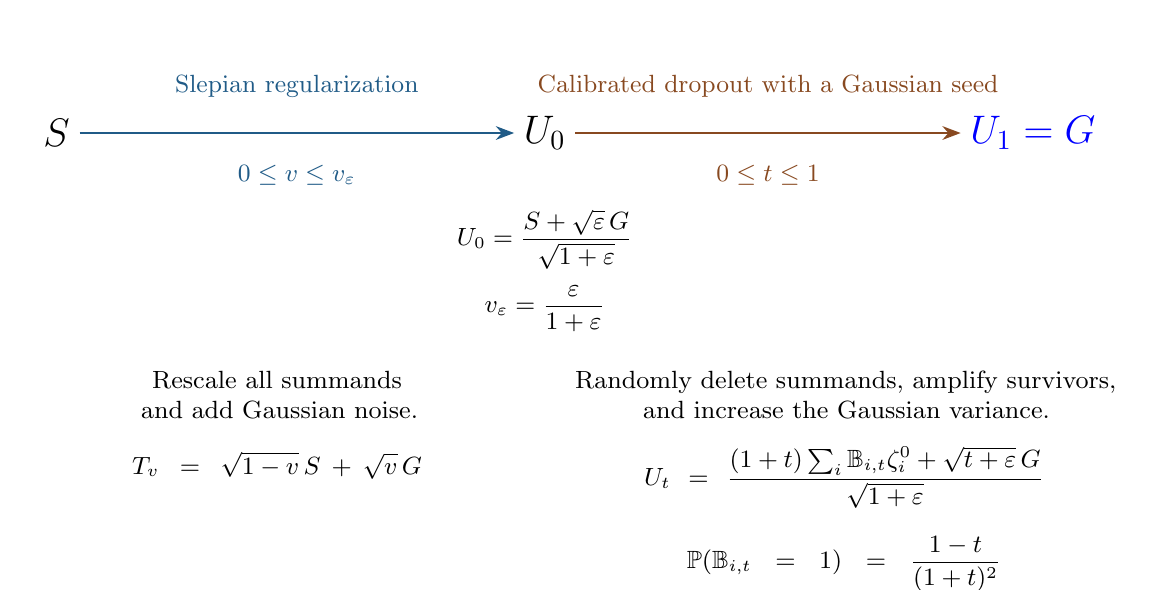
\begin{tikzpicture}[>=Stealth,font=\fontsize{9}{11}\selectfont]
\definecolor{seed}{RGB}{32,91,135}
\definecolor{drop}{RGB}{136,73,32}
\node[font=\Large] (S) at (0,0) {$S$};
\node[font=\Large] (U) at (6.2,0) {$U_0$};
\node[font=\Large] (G) at (12.4,0) {$\textcolor{blue}{U_1=G}$};
\draw[->,thick,seed] (S) -- node[above=9pt,align=center] {Slepian regularization} node[below=8pt] {$0\le v\le v_\varepsilon$} (U);
\draw[->,thick,drop] (U) -- node[above=9pt,align=center] {Calibrated dropout with a Gaussian seed} node[below=8pt] {$0\le t\le1$} (G);
\node[anchor=north,align=center] at (6.2,-0.85) {$\displaystyle U_0=\frac{S+\sqrt\varepsilon\,G}{\sqrt{1+\varepsilon}}$
\\[5pt] $\displaystyle v_\varepsilon=\frac{\varepsilon}{1+\varepsilon}$};
\node[anchor=north,align=center,text width=6.1cm] at (2.8,-2.9) {Rescale all summands\\and add Gaussian noise.\\[9pt]
 $\displaystyle T_v=\sqrt{1-v}\,S+\sqrt v\,G$};
\node[anchor=north,align=center,text width=7.0cm] at (10,-2.9) {Randomly delete summands, amplify survivors,\\and increase the Gaussian variance.\\[9pt]
 $\displaystyle U_t=\frac{(1+t)\sum_i\mathbb B_{i,t}\zeta_i^0+\sqrt{t+\varepsilon}\,G}{\sqrt{1+\varepsilon}}$\\[9pt]
 $\displaystyle \mathbb P(\mathbb B_{i,t}=1)=\frac{1-t}{(1+t)^2}$};
\end{tikzpicture}
}
\caption{The comparison from \(S\) to \(G\) passes through the regularized
sum \(U_0\). The first stage follows \(T_v\) up to \(v_\varepsilon\),
and the second follows \(U_t\) from \(t=0\) to \(t=1\),
\textcolor{blue}{ending at \(U_1=G\)}.}
\label{fig:two-stage-path}
\end{figure}

{Fix \(\varepsilon>0\). In the first stage, we rescale \(S\)
and add a small independent Gaussian component along the
\emph{Slepian interpolation}}
\[
 T_v\coloneqq\sqrt{1-v}\,S+\sqrt v\,G,
 \qquad 0\le v\le1.
\]
{We stop at time \(v_\varepsilon\coloneqq\varepsilon/(1+\varepsilon)\),
so the first stage starts at \(T_0=S\) and ends at}
\[
 U_0\coloneqq T_{v_\varepsilon}
 =\frac{S+\sqrt\varepsilon\,G}{\sqrt{1+\varepsilon}}.
\]
{Since \(S\) and \(G\) are independent and both have covariance
\(I_r\), we have \(\Cov(T_v)=(1-v)I_r+vI_r=I_r\) throughout this stage.}

\begin{samepage}
{The initial independent Gaussian component, which we call the
\emph{Gaussian seed}, contributes \(\varepsilon I_r/(1+\varepsilon)\)
to the covariance of \(U_0\). This seed gives the second stage a positive
Gaussian variance from its starting point, permitting two Gaussian
integrations by parts throughout that stage, including at \(t=0\).
We call the initial operation \emph{Slepian regularization}.}
After a change of time it is also
\emph{Ornstein--Uhlenbeck regularization}~\cite[Theorem~4.12]{Nourdin2012}.
\par
\end{samepage}

{Starting from \(U_0\), we now delete summands at random,
rescale those retained, and increase the Gaussian variance.
For each time \(t\in[0,1]\), let \(\mathbb B_{i,t}\) be independent Bernoulli
\emph{masks}, independent of the summands and \(G\), and define}
\begin{equation}
 U_t\coloneqq
 \frac{(1+t)\sum_{i=1}^n\mathbb B_{i,t}\zeta_i^0
             +\sqrt{t+\varepsilon}\,G}{\sqrt{1+\varepsilon}},
 \qquad 0\le t\le1.
 \label{eq:path}
\end{equation}
A mask equal to \(1\) retains its summand, and a mask equal to zero deletes it.
Before the common normalization, each retained summand is multiplied by its
\emph{amplitude} \(\gamma(t)\coloneqq1+t\).

The \emph{retention probability} is
\[
 \varpi(t)\coloneqq\Pp(\mathbb B_{i,t}=1)
             =\frac{1-t}{(1+t)^2}.
\]
These choices give \(\varpi(t)\gamma(t)^2=1-t\). In the normalized
path~\eqref{eq:path}, the two independent components therefore contribute
{covariances adding up to \(I_r\):}
\[
 \underbrace{\frac{1-t}{1+\varepsilon}I_r}_{\text{retained summands}}
 +\underbrace{\frac{t+\varepsilon}{1+\varepsilon}I_r}_{\text{Gaussian component}}
 =I_r.
\]
As \(t\) increases, covariance is transferred from the retained summands
to the Gaussian component, while \(\Cov(U_t)=I_r\) throughout.
{At \(t=0\), every summand is retained, giving the regularized
sum \(U_0\) constructed in the first stage. At \(t=1\), all summands have
been deleted and \(U_1=G\).}

{The joint choice of amplitude and retention probability also
controls the third-moment contribution. Before normalization, each summand's
third-moment tensor is multiplied by}
\[
 {\varpi(t)\gamma(t)^3=1-t^2.}
\]
{The derivative of this multiplier vanishes at \(t=0\),
which helps control the third moments when the Gaussian variance is smallest.}
This random deletion is known as \emph{Bernoulli thinning}
\cite{Renyi1956,SteutelHarn1979,LastPenrose2017}. We call the
chosen amplitude and retention probability \emph{calibrated dropout},
in reference to the independent masks used in dropout regularization~\cite{Dropout2014}.
With \(\varepsilon=0\), this coincides with the calibrated path
defined in~\cite[Section~4]{AL}.
The paths describe distributions at each time, and
we do not need to couple the Bernoulli masks across different times.

{
To measure changes in the smoothed probabilities along the first stage, {define}
\[
 P_a^0(v)\coloneqq\E F_{a,h}(T_v),\qquad 0\le v\le1.
\]
The superscript \(0\) labels this initial stage. Since
\(T_0=S\) and \(T_{v_\varepsilon}=U_0\), the cost of introducing the seed
can be bounded by integrating the rate of change:
\[
 I_h\coloneqq\sup_a|P_a^0(v_\varepsilon)-P_a^0(0)|
 =\sup_a\left|\int_0^{v_\varepsilon}(P_a^0)'(v)\,dv\right|
 \le\sup_a\int_0^{v_\varepsilon}|(P_a^0)'(v)|\,dv.
\]
}

{To measure the change in the smoothed probabilities along the
second stage, {define}}
\[
 P_a(t)\coloneqq\E F_{a,h}(U_t).
\]
{
Its derivative \(P_a'(t)\) is the rate of change at time \(t\).
The two stages meet at \(P_a^0(v_\varepsilon)=P_a(0)\).
The triangle inequality and integration along the paths therefore give
\begin{equation}
\begin{aligned}
 M_h&\le I_h+\sup_a\int_0^1|P_a'(t)|\,dt\\
 &\le
 \underbrace{\sup_a\int_0^{v_\varepsilon}|(P_a^0)'(v)|\,dv}
             _{\text{Slepian regularization}}
 +\underbrace{\sup_a\int_0^1|P_a'(t)|\,dt}
             _{\text{calibrated dropout}}.
\end{aligned}
\label{eq:roadmap}
\end{equation}
It remains to bound the two derivatives over their respective time intervals.
}

\subsection{Controlling the comparison error}
\label{sec:outline-seeded}

{
We bound the two integrals in~\eqref{eq:roadmap} in the order of the
comparison. {The initial Slepian stage is controlled by direct averaged derivative estimates.} Its purpose is to introduce
the Gaussian seed needed for the main comparison. {Using this seed, we will obtain derivative bounds in the second stage.}

Let
\[
 K_3\coloneqq\sum_i\E(\zeta_i^0)^{\otimes3}
\]
denote the aggregate third-moment tensor.
{
Here \(z^{\otimes3}\) has entries \(z_jz_kz_\ell\).
}
Along the initial Slepian path,
Lemma~\ref{appx-an:lem:identity} separates its contribution from the
fourth-order remainder:
\[
 (P_a^0)'(v)
 =-\frac{\sqrt{1-v}}4\E D^3F_{a,h}(T_v):K_3+R^0_{a,h}(v),
 \qquad 0<v<1.
\]
{
The contraction \(D^3F(x):K_3\) is the sum of the third partial
derivatives of \(F\) at \(x\), each multiplied by the corresponding
entry of \(K_3\). We similarly write
\(D^qF(x)[z_1,\ldots,z_q]\) for the \(q\)th derivative evaluated in
the listed directions. The term \(R^0_{a,h}\) is the integral
remainder supplied by the lemma.
}

{
The derivative bounds improve after averaging because the logistic
 derivatives are concentrated near the smoothed boundary. Each spatial
 derivative contributes a factor \(h^{-1}\), giving the pointwise factors
 \(h^{-3}\) and \(h^{-4}\) for the third and fourth derivatives.
 However, their expansions also contain positive logistic weight products
 whose sums are bounded by a constant times
\[
 F_{a,h}(x)\bigl(1-F_{a,h}(x)\bigr).
\]
This weight is appreciable only where the smoother transitions between
\(0\) and \(1\). We will show that its expectation along the Slepian
path is at most \(Ch\vSix{\kappa}\). Multiplying by this bound improves the
 derivative factors from \(h^{-3}\) and \(h^{-4}\) to
\(h^{-2}\vSix{\kappa}\) and \(h^{-3}\vSix{\kappa}\), respectively.

{
To bound this expected weight, fix \(x\) and increase all thresholds
by the same amount \(s\). Define
\(F_s(x):=F_{a+s\mathbf1,h}(x)\), where \(\mathbf1\in\R^m\)
has all entries equal to \(1\). Direct differentiation gives
\[
 \frac{\partial}{\partial s}F_s(x)
 =h^{-1}F_s(x)\{1-F_s(x)\}.
\]
For \(|s|\le h\), the product \(F_s(x)\{1-F_s(x)\}\) is at least
\(e^{-1}F_0(x)\{1-F_0(x)\}\). Integrating over \([-h,h]\) yields
\[
 F_0(x)\{1-F_0(x)\}
 \le \frac e2\{F_h(x)-F_{-h}(x)\}.
\]
By~\eqref{eq:mixture}, \(F_h(x)-F_{-h}(x)\) is the probability,
over the random shifts \(\omega\), that \(x\) belongs to the shell
\(A_{a,\omega}^{h}\setminus A_{a,\omega}^{-h}\).

We apply this inequality at \(T_v=\sqrt{1-v}\,S+\sqrt v\,G\).
The two independent components have variances \(1-v\) and \(v\)
along every face normal. Condition on the component with the smaller
variance and on the random thresholds. The remaining component has
variance at least \(1/2\) along every face normal. \vSix{Its expected face norm is at most
\(\E\|W\|_\infty\) or \(g_\Sigma\), respectively, so the intrinsic
and dimension-based parts of Lemma~\ref{lem:concentration}} bound the conditional shell probability
by \(C(h+\delta)\vSix{\kappa}\). Hence, uniformly in \(v\),
\[
 \E[F_{a,h}(T_v)\{1-F_{a,h}(T_v)\}]
 \le C(h+\delta)\vSix{\kappa}\le Ch\vSix{\kappa},
 \qquad {h\ge\delta}.
\]
The smoothing error compares \(A_{a,\omega}\) with \(A_a\), and
therefore depends on the largest absolute random threshold shift.
Here we compare \(A_{a,\omega}^{h}\) with \(A_{a,\omega}^{-h}\):
each corresponding pair of thresholds differs by exactly \(2h\),
regardless of the random shifts.
}

We now combine this averaging bound with the relative moment bounds
in~\eqref{eq:relative-moments}. The cubic contribution is controlled by
\(s_3\), which measures the aggregate third moments and retains
cancellation across summands. The fourth-order remainder is controlled
by \(s_4\). To apply the same averaging bound to this remainder, we must
also account for the shifts in its derivative evaluation points.
These shifts change each scalar product \(u_\alpha\cdot x\) by at most
\(C\delta\). {Since \(h\ge\delta\)}, the shifted logistic weights
can therefore be compared with those at \(T_v\), losing only an
absolute constant. Appendix~\ref{appx-an:sec:initialization} supplies the details.
}

Combining the derivative factors with the averaged boundary weight
gives
\[
\begin{aligned}
 \left|\E D^3F_{a,h}(T_v):K_3\right|
 &\le Cs_3h^{-3}\,h\vSix{\kappa}
 =\frac{Cs_3\vSix{\kappa}}{h^2},\\
 |R^0_{a,h}(v)|
 &\le Cs_4h^{-4}\,h\vSix{\kappa}
 =\frac{Cs_4\vSix{\kappa}}{h^3}.
\end{aligned}
\]
Thus averaging supplies one factor of \(h\) before we integrate over
time. Substituting these estimates into the Slepian identity yields
\[
 |(P_a^0)'(v)|
 \le C\vSix{\kappa}\left(\frac{s_3}{h^2}+\frac{s_4}{h^3}\right),
 \qquad 0<v<1.
\]

{
The first stage lasts only until \(v_\varepsilon\le\varepsilon\),
so integration gives
\[
 I_h\le C\varepsilon\vSix{\kappa}
       \left(\frac{s_3}{h^2}+\frac{s_4}{h^3}\right).
\]
For fixed \(h\), increasing \(\varepsilon\) increases the stopping
time \(v_\varepsilon\) and the displayed bound on \(I_h\). We choose
\(\varepsilon\) after examining how the factor \(t+\varepsilon\)
enters the derivative bounds obtained by Gaussian integration by parts.
}

For the calibrated dropout path, the same lemma gives}

\begin{equation}
 P_a'(t)=
 -\frac{t}{3(1+\varepsilon)^{3/2}}\,
       \E D^3F_{a,h}(U_t):K_3+R_{4,a,h}(t).
 \label{eq:path-summary}
\end{equation}
{
{
{
The remainder \(R_{4,a,h}(t)\) consists of fourth derivatives evaluated
at shifted points \(U_t+\Delta\). Here \(\Delta\) denotes the random
displacement obtained by deleting one scaled summand and inserting a
scaled independent copy along the segment in Taylor's formula. It
depends on the summand index and the position along that segment, and
may depend on the same summands as \(U_t\) and the derivative
directions. Formula~\eqref{appx-an:translates} gives these displacements
before the normalization by \(\sqrt{1+\varepsilon}\). Every such shift
changes each face projection by at most \(C\delta\):
\[
 \max_{\alpha\le m}|u_\alpha\cdot\Delta|\le C\delta.
\]
}
} To see how the Gaussian component helps, write \(F=F_{a,h}\),
let \(g\sim N(0,I_r)\), and fix a base point \(x\in\R^r\), directions
\(z,w_1,w_2\in\R^r\), and a scale \(\sigma>0\). Two Gaussian integrations
by parts give
\[
\begin{aligned}
 &\E_g D^4F(x+\sigma g)[z,z,w_1,w_2]\\
 &\qquad=\frac1{\sigma^2}\,
 \E_g\!\left[
 \bigl\{(g\cdot z)^2-\norm z^2\bigr\}
 D^2F(x+\sigma g)[w_1,w_2]
 \right].
\end{aligned}
\]
We apply this identity after conditioning on the base and derivative
directions. It replaces two derivatives of the logistic approximation
by the \emph{Hermite term} \((g\cdot z)^2-\norm z^2\).
In our application, \(\sigma^2\) is comparable to \(t+\varepsilon\),
so these integrations contribute \((t+\varepsilon)^{-1}\), while the
two remaining derivatives contribute \(h^{-2}\).

{
To connect this identity to the fourth-moment assumption, we expand the
 two remaining derivatives. Their logistic weights are multiplied by
 face projections, such as \(u_j\cdot w_1\) and \(u_k\cdot w_2\).
When all four directions equal the same summand \(\zeta_i^0\), a term
involving \((u_j\cdot\zeta_i^0)^2\) combines with the Hermite term as
\[
\begin{aligned}
 &(u_j\cdot\zeta_i^0)^2
 \bigl\{(g\cdot\zeta_i^0)^2-\norm{\zeta_i^0}^2\bigr\}\\
 &\qquad=\tr\!\left[
 (gg^\top-I_r)(u_j\cdot\zeta_i^0)^2
 \zeta_i^0(\zeta_i^0)^\top
 \right].
\end{aligned}
\]
The sum of the expected coefficient matrices is
\[
 A_j:=\sum_i\E\!\left[
 (u_j\cdot\zeta_i^0)^2\,
 \zeta_i^0(\zeta_i^0)^\top
 \right]\preceq s_4I_r,
\]
by the fourth-moment bound in~\eqref{eq:relative-moments}, expressed in
support coordinates. Terms involving different face normals or
independent copies satisfy analogous operator-norm bounds.
{
A related use of aggregate matrix bounds after two Gaussian
integrations by parts appears in~\cite[Lemma~16]{GaoZhang}.
Here we also need to retain the boundary-concentration gain,
which requires the weighted Gaussian estimates developed in
Appendix~\ref{appx-sec:support}.
}
}

{
The inequality \(A_j\preceq s_4I_r\) controls the moment
coefficients. The remaining task is to bound the Gaussian
expectation of the Hermite term multiplied by the logistic weights.
Both factors depend on the same Gaussian vector, so we cannot
multiply their separate expectation bounds.
Estimating their absolute sizes separately would also lose the
cancellations needed to avoid a factor depending on rank.
The matrix and threshold estimates in
Appendix~\ref{appx-sec:support} control the Gaussian matrix
\(gg^\top-I_r\) averaged against the products of logistic
probabilities arising from the derivatives. Under the scale
conditions of Proposition~\ref{an:prop:derivative} {below}, these estimates
supply a factor \(Ch\vSix{\kappa L}\) in the remainder bound, with no factor
depending on \(r\). The corresponding factor without the Hermite
term was \(Ch\vSix{\kappa}\).
Consequently,
\[
 |R_{4,a,h}(t)|
 \le Cs_4\,\frac1{t+\varepsilon}\,\frac1{h^2}\,h\vSix{\kappa L}
 =\frac{Cs_4\vSix{\kappa L}}{h(t+\varepsilon)}.
\]
Thus the boundary gain of one power of \(h\) survives the two
integrations by parts, at the cost of an additional factor \(L\)
in this weighted estimate.

For the cubic contribution, two Gaussian integrations by parts
leave one derivative of \(F_{a,h}\), which contributes \(h^{-1}\).
The signed aggregate third-moment matrices supply the factor
\(s_3\). Multiplying by the weighted boundary factor \(h\vSix{\kappa L}\)
removes this remaining power of \(h^{-1}\).
Including the coefficient in~\eqref{eq:path-summary} gives a bound
\(Cs_3\vSix{\kappa L}t/(t+\varepsilon)\).
The derivative of the calibrated third-moment multiplier
\(1-t^2\) supplies the factor \(t\). Since \(t/(t+\varepsilon)\le1\),
integration over \(0\le t\le1\) contributes at most \(Cs_3\vSix{\kappa L}\),
uniformly in the seed \(\varepsilon\). The fourth-order bound
has no compensating factor \(t\), and its integral contains
\(\log(1+1/\varepsilon)\).

We choose the seed scale by comparing the errors accumulated over
both stages. The direct derivative bounds are useful during the short
initialization stage: although its fourth-order bound contains
\(h^{-3}\), it is integrated over an interval of length at most
\(\varepsilon\). Its fourth-order contribution is therefore bounded by
\(C\varepsilon s_4\vSix{\kappa}/h^3\). Choosing \(\varepsilon=Lh^2\)
makes this contribution at most \(Cs_4\vSix{\kappa L}/h\), and the full
first-stage bound becomes
\[
 I_h\le C\vSix{\kappa L}\left(s_3+\frac{s_4}{h}\right).
\]
Thus the short duration compensates for the unfavorable powers of
\(h\) in the direct derivative bounds.

With this seed choice, the fourth-order bound in the second stage
can be written as
\[
 |R_{4,a,h}(t)|
 \le \frac{Cs_4\vSix{\kappa}}{h^3}\,
       \frac{\varepsilon}{t+\varepsilon}.
\]
It has the same order as the direct derivative bound at \(t=0\),
but decreases as the Gaussian variance grows. Consequently,
\[
 \sup_a\int_0^1|R_{4,a,h}(t)|\,dt
 \le \frac{Cs_4\vSix{\kappa L}}h
       \log\!\left(1+\frac1\varepsilon\right).
\]
A larger seed would increase the initialization bound linearly while
reducing the second-stage logarithm. The choice \(\varepsilon=Lh^2\)
keeps the fourth-order initialization cost at the scale
\(s_4\vSix{\kappa L}/h\), and the second stage costs this scale times a
logarithm. The gain comes from accumulating the direct bound only
over a short interval and using the decreasing Gaussian bound for
the rest of the comparison.
The next proposition states these bounds under their precise
scale conditions.
}

}

\begin{proposition}[Initialization and seeded derivative estimates]
\label{an:prop:derivative}
\vSix{Under~\eqref{eq:setup} and \eqref{eq:relative-moments}, with
\(\kappa\) defined in~\eqref{eq:intrinsic-boundary-coefficient}, there are absolute constants} \(\mathsf A,C\)
such that, for \(h\ge\mathsf A\delta\), uniformly over
\(a\in\R^m\) and \(0<v<1\),
\begin{equation}
 |\E D^3F_{a,h}(T_v):K_3|\le\frac{Cs_3\vSix{\kappa}}{h^2},
 \qquad |R^0_{a,h}(v)|\le\frac{Cs_4\vSix{\kappa}}{h^3}.
 \label{eq:direct-initialization}
\end{equation}
If \(Lh^2<1/4\), choose \(\varepsilon=Lh^2\) in~\eqref{eq:path}.
Then
\begin{equation}
 I_h\le Cs_3 \vSix{\kappa L}+\frac{Cs_4\vSix{\kappa L}}h,
 \label{eq:initialization-bound}
\end{equation}
and, uniformly over \(a\in\R^m\) and \(0<t<1\),
\begin{equation}
 \begin{aligned}
 \left|\frac{t}{3(1+\varepsilon)^{3/2}}
          \E D^3F_{a,h}(U_t):K_3\right|
 &\le Cs_3 \vSix{\kappa L}\frac{t}{t+\varepsilon},\\
 |R_{4,a,h}(t)|&\le\frac{Cs_4\vSix{\kappa L}}{h(t+\varepsilon)}.
 \end{aligned}
 \label{eq:seeded-derivatives}
\end{equation}

\end{proposition}
\subsection{\vSix{Proof of Theorem~\ref*{thm:unrestricted}}}\label{sec:proof-theorem-one}

\begin{vSixBlock}
\begin{proof}[Proof of Theorem~\ref{thm:unrestricted}]
We combine the errors from smoothing and the two comparison stages,
then choose the smoothing width to balance their contributions.
The envelope condition allows us to take \(s_3\le\delta\).

First fix \(h\ge\mathsf A\delta\), where \(\mathsf A\ge1\) is the
constant in Proposition~\ref{an:prop:derivative}, and suppose that
\(Lh^2<1/4\). Set \(\varepsilon\coloneqq Lh^2\). By the smoothing
bound~\eqref{eq:endpoint-min} and the decomposition~\eqref{eq:roadmap},
\[
 \rh(W,Z)
 \le Ch\kappa L+I_h+\sup_a\int_0^1|P_a'(t)|\,dt.
\]
The first term is the smoothing error. For the initial Slepian stage,
\eqref{eq:initialization-bound} gives
\[
 I_h\le C\kappa L\left(s_3+\frac{s_4}{h}\right).
\]
For the calibrated dropout stage, we integrate the cubic and
fourth-order bounds in~\eqref{eq:seeded-derivatives}. Their time
integrals behave differently:
\[
 \int_0^1\frac{t}{t+\varepsilon}\,dt\le1,
 \qquad
 \int_0^1\frac{dt}{t+\varepsilon}
 =\log\!\left(1+\frac1\varepsilon\right).
\]
Thus the cubic contribution has a bounded time integral, whereas the
fourth-order remainder contributes a logarithm. Combining the two
stages with the smoothing error yields
\[
 \rh(W,Z)\le C\kappa L\left[
 h+s_3+\frac{s_4}{h}
 \left\{1+\log\!\left(1+\frac1{Lh^2}\right)\right\}
 \right].
\]

We now choose \(h\). Since \(h\ge\delta\),
\[
 1+\log\!\left(1+\frac1{Lh^2}\right)
 \le1+\log\!\left(1+\frac1{L\delta^2}\right)
 \le CD_L.
\]
Using also \(s_3\le\delta\), we obtain
\[
 \rh(W,Z)\le C\kappa L
 \left(h+\delta+\frac{s_4D_L}{h}\right).
\]
Increasing \(h\) enlarges the smoothing error but reduces the
fourth-order contribution. Balancing these terms, subject to
\(h\ge\mathsf A\delta\), leads to
\[
 h\coloneqq\mathsf A\max\{\delta,\sqrt{s_4D_L}\}.
\]
For this choice,
\[
 h+\delta+\frac{s_4D_L}{h}
 \le C\left(\delta+\sqrt{s_4D_L}\right).
\]
If \(Lh^2<1/4\), the preceding estimates, together with
\(\rh(W,Z)\le1\), give \(\rh(W,Z)\le C\kappa L(\delta+\sqrt{s_4D_L})\).

It remains to cover the case in which the chosen width satisfies
\(Lh^2\ge1/4\). Then
\[
 \kappa L\left(\delta+\sqrt{s_4D_L}\right)
 \ge\frac{\kappa Lh}{\mathsf A}
 \ge\frac{\kappa\sqrt L}{2\mathsf A}
 \ge\frac1{2\mathsf A}.
\]
Since \(\kappa\ge1\) and \(L\ge1\), the same bound follows
from \(\rh(W,Z)\le1\) in this case.

We now express \(\kappa\) through the Gaussian width. If
\(\delta L\le g_\Sigma\), Lemma~\ref{intrinsic:lem:maximum} and
\(g_\Sigma\ge\sqrt{2/\pi}\) give \(\kappa\le Cg_\Sigma\).
Otherwise, \(\delta g_\Sigma L>g_\Sigma^2\ge2/\pi\), so
\eqref{eq:intrinsic-unrestricted} follows directly from
\(\rh(W,Z)\le1\). This proves~\eqref{eq:intrinsic-unrestricted}
in both cases. Finally, the envelope condition permits
\(s_4=\delta^2\). Substitution and \(D_L\ge1\) give
\eqref{eq:intrinsic-envelope}.
\end{proof}
\end{vSixBlock}

\begin{vSixBlock}
The factor \(L\) outside the final square root comes from the
random threshold shifts and the Gaussian weighted derivative estimates.
Theorem~\ref{opt:symmetric-lower} shows that a factor of this order
is necessary even when Gaussian width is bounded. The additional
logarithm inside \(D_L\) comes from integrating the fourth-order
remainder near the beginning of the second stage. Its necessity
remains open.
\end{vSixBlock}

\section{Outline of the Proof of Theorem~\ref*{thm:polynomial}}\label{sec:poly}

\begin{recovered}
We prove part~\textup{(i)} of Theorem~\ref{thm:polynomial} by
conditional truncation and part~\textup{(ii)} by a refinement of the
polynomial-moment estimate in~\cite{CCKK2022}. The first argument
uses only the envelope condition~\eqref{poly:envelope}. The second
also uses the coordinate fourth-moment condition~\eqref{poly:fourth}
in a Bennett inequality. We outline the two arguments below and
compare their rates. Appendix~\ref{app:polynomial-proof} gives
both proofs, in Subsections~\ref{app:conditional}
and~\ref{app:bennett}, respectively.
\end{recovered}

Throughout this section, \(W,Z,\Sigma\), and \(L\) have the meanings
in~\eqref{poly:setup}. Let \(\mathcal E_q(B,p)\) be the class of
independent centered arrays with unit average marginal variances
satisfying the envelope condition~\eqref{poly:envelope}, without
requiring~\eqref{poly:fourth}. Thus
\(\mathcal C_q(B,p)\subseteq\mathcal E_q(B,p)\).
To shorten the proof calculations, define
\begin{equation}
 \alpha_q:=\frac12-\frac1q,\qquad
 V_q:=\frac{B L^{3/2-1/q}}{n^{1/2-1/q}}
      =Bn^{-\alpha_q}L^{1+\alpha_q}.
 \label{poly:rates}
\end{equation}
\vSix{The quantity \(V_q\) records the dimension-based scale.
The intrinsic upper bounds below retain the additional factor
\(g_\Sigma/\sqrt L\).}
The moment order \(q>2\) is fixed. Constants indexed by \(q\)
may depend on it, and the bounds are not asserted uniformly as
\(q\) approaches \(2\) or infinity.

\subsection{\texorpdfstring{{Part (i): transfer from bounded observations}}{Part (i): transfer from bounded observations}}\label{poly:transfer-sec}

Truncating all {summands} and paying the probability that any {summand} changes
loses information about the size of the exceptional observations.
Instead, we condition on which {summands} are exceptional. Given this
information, the remaining {summands} are independent and bounded, and the
exceptional part can be treated as a random shift. The bounded-summand
theorem and Gaussian anti-concentration then control the two parts.
\vSix{The conditional covariance is dominated by a fixed multiple of
\(\Sigma\), which keeps its Gaussian width bounded by \(Cg_\Sigma\).
Comparisons obtained by adding independent Gaussian vectors control
the covariance correction with the same width factor.}

\begin{recovered}
In the notation above, the conclusion~\eqref{poly:main-envelope} of
Theorem~\ref{thm:polynomial}\textup{(i)} becomes
\begin{equation}
 \vSix{\rh(W,Z)\le C_q\min\{1,(g_\Sigma/\sqrt L)
               V_q\{\log(en)\}^{\alpha_q}\},}
 \qquad (X_i)_{i=1}^n\in\mathcal E_q(B,p).
 \label{poly:transfer-bound}
\end{equation}
Appendix~\ref{app:conditional} proves this bound by choosing the
truncation threshold to balance the approximation error for bounded
observations against the variance discarded in the tails. The extra
logarithm in~\eqref{poly:transfer-bound} comes from the
bounded-observation theorem. If Conjecture~\ref{conj:sharp-unrestricted}
holds, the same argument gives \(C_q\min\{1,V_q\}\)
\vSix{in the worst case over covariance matrices}, under the
envelope condition alone {(see Remark~\ref{rmk:E1})}.
\end{recovered}

\subsection{\texorpdfstring{{Part (ii): refinement under coordinate fourth moments}}{Part (ii): refinement under coordinate fourth moments}}\label{poly:bennett-sec}

\begin{recovered}
Coordinate fourth moments can be substantially smaller than the fourth
moment of the random envelope. Adding the coordinate condition
\eqref{poly:fourth} restricts the class from \(\mathcal E_q(B,p)\)
to \(\mathcal C_q(B,p)\) and permits a sharper treatment of large
observations. To express this improvement, define
\end{recovered}
\begin{equation}
 U:=\frac{B^{1/2}L^{5/4}}{n^{1/4}},\qquad
 \mathcal K_q:=\left(\frac{V_q}{U}\right)^2
     =B\left(\frac nL\right)^{2/q-1/2},\qquad
 \mathcal L_q:=\log(e+\mathcal K_q).
 \label{poly:bennett-parameters}
\end{equation}
Under~\eqref{poly:envelope} and~\eqref{poly:fourth}, the bound of
Chernozhukov, Chetverikov, Kato, and
Koike~\cite[Theorem~2.5]{CCKK2022} gives
\(\rh(W,Z)\le C_q\min\{1,U+V_q\}\).
Its rectangle form follows by applying their lower-orthant bound
to \((X_i,-X_i)\). This preserves the moment bounds, and
\(\log(2p)\) is comparable to \(L\).
The quantity \(\mathcal K_q\) compares the two contributions.
When it is large, Bennett's inequality reduces the envelope
contribution by a power of \(\mathcal L_q\).

\begin{recovered}
In this notation, the conclusion~\eqref{poly:main-fourth} of
Theorem~\ref{thm:polynomial}\textup{(ii)} becomes
\begin{equation}
 \rh(W,Z)\le C_q\min\left\{1,
 \vSix{\frac{g_\Sigma}{\sqrt L}
 \left(U+\frac{V_q}{\mathcal L_q^{1-1/q}}\right)}\right\},
 \qquad (X_i)_{i=1}^n\in\mathcal C_q(B,p).
 \label{poly:bennett-bound}
\end{equation}
The proof compares logistic approximations along a Slepian path.
Interchanging each summand with an independent copy gives a
fourth-order remainder, and a Bennett inequality controls the large
increments. The variance estimate uses both \eqref{poly:envelope}
and \eqref{poly:fourth}. \vSix{Gaussian anti-concentration contributes
the common factor \(g_\Sigma\) to every term of the comparison,
so retaining width does not change the bandwidth choices or
\(\mathcal K_q\).} Appendix~\ref{app:bennett} gives a
self-contained proof of the comparison estimate and the refinement.
\end{recovered}
Basu and Kuchibhotla use a related truncation
argument for maxima of independent sums~\cite[Proposition~4.2]{BK2025}.

\begin{recovered}
The two appendix proofs give the respective parts of
Theorem~\ref{thm:polynomial}. Taking the larger of their constants
as \(C_q\) makes both bounds valid on \(\mathcal C_q(B,p)\),
where we may therefore take their minimum. Table~\ref{poly:summary}
summarizes the assumptions, proof routes, and lower-bound comparisons.
\end{recovered}

\begin{table}[htbp]
\centering

\small
\renewcommand{\arraystretch}{1.15}
\begin{tabularx}{\textwidth}{@{}>{\raggedright\arraybackslash}p{0.23\textwidth}
 >{\raggedright\arraybackslash}p{0.27\textwidth}
 >{\raggedright\arraybackslash}X@{}}
\toprule
Result, assumptions, and upper rate & Proof route & Lower bounds and remaining gap\\
\midrule
Theorem~\ref{thm:polynomial}\textup{(i)}\newline
Condition~\eqref{poly:envelope} alone\newline
\vSix{\((g_\Sigma/\sqrt L)V_q\{\log(en)\}^{\alpha_q}\)}
& Conditional truncation, followed by the bounded-summand theorem and
Gaussian anti-concentration.\newline Appendix~\ref{app:conditional}.
& Theorem~\ref{lower:dense}\textup{(i)} gives a lower bound of order
\vSix{\((g_\Sigma/\sqrt L)V_q\)} for every fixed \(q>2\),
with fixed or growing \(B\ge2\).
The remaining factor is \(\{\log(en)\}^{\alpha_q}\), whose
necessity is unresolved.\\[0.6em]
Theorem~\ref{thm:polynomial}\textup{(ii)}\newline
Conditions~\eqref{poly:envelope} and~\eqref{poly:fourth}\newline
\vSix{\((g_\Sigma/\sqrt L)(U+V_q/\mathcal L_q^{1-1/q})\)}
& Logistic smoothing, Slepian interpolation with paired increments, and
a Bennett inequality using both moment conditions.\newline
Appendix~\ref{app:bennett}.
& Matching lower bounds for fixed \(B\ge2\) at \(q=4\)
(Theorem~\ref{opt:q4-lower}) and for large \(\mathcal K_q\)
(Theorem~\ref{lower:sparse}). At \(q=4\),
Theorem~\ref{opt:q4-growing} also matches the dependence on growing \(B\).\\
\bottomrule
\end{tabularx}
\caption{The two parts of Theorem~\ref{thm:polynomial}, their proofs,
and their sharpness. Constants are suppressed and both upper bounds
are capped at 1. \vSix{The lower-bound examples have widths
ranging from a constant to order \(\sqrt L\), subject to the
dimension and vanishing-rate conditions in Section~\ref{opt:section}.}}
\label{poly:summary}
\end{table}

\subsection{\texorpdfstring{{Comparison of the bounds under the two moment assumptions}}{Comparison of the bounds under the two moment assumptions}}\label{poly:transition}

\begin{vSixBlock}
Both upper bounds retain the factor \(g_\Sigma/\sqrt L\), so
their relative sizes are determined by \(U,V_q,\mathcal K_q\),
and \(\mathcal L_q\). The lower bounds use the same width factor.
The comparisons below apply along the dimension and width sequences
specified in Section~\ref{opt:section}.

Under the envelope condition alone, Theorem~\ref{lower:dense}\textup{(i)}
gives a lower bound of order \((g_\Sigma/\sqrt L)V_q\) for
every fixed \(q>2\) and fixed or growing \(B\ge2\), when this
scale tends to zero. The bound~\eqref{poly:transfer-bound} differs
by the factor \(\{\log(en)\}^{\alpha_q}\).

When the coordinate fourth-moment condition also holds, both bounds
are available. First fix \(B\ge2\) and suppose \(n/L\to\infty\).
For \(2<q<4\), we have \(\mathcal K_q\to\infty\), and
\[
 \frac{V_q/\mathcal L_q^{1-1/q}}U
 =\frac{\sqrt{\mathcal K_q}}{\mathcal L_q^{1-1/q}}\to\infty.
\]
Thus~\eqref{poly:bennett-bound} has order
\((g_\Sigma/\sqrt L)V_q/\mathcal L_q^{1-1/q}\), improving
the logarithmic factors in~\eqref{poly:transfer-bound}.
Theorem~\ref{lower:sparse} matches this rate from below when
\(\log\mathcal K_q=o(L)\) and the intrinsic rate tends to zero.

At \(q=4\), \(\mathcal K_4=B\), and the second term absorbs
the first uniformly in \(B\ge1\), because
\(\{\log(e+B)\}^{3/4}/\sqrt B\) is bounded. Hence
\begin{equation}
 \rh(W,Z)\le C\min\left\{1,
 \frac{g_\Sigma Bn^{-1/4}L^{3/4}}
 {\{\log(e+B)\}^{3/4}}\right\}.
 \label{poly:q4}
\end{equation}
For fixed \(B\ge2\), Theorem~\ref{opt:q4-lower} matches
\(g_\Sigma n^{-1/4}L^{3/4}\) from below. In particular,
\(n^{-1/4}L^{3/4}\) is sharp even when width stays bounded.
For growing \(B\), Theorem~\ref{opt:q4-growing} also matches
the factor \(B/\{\log(e+B)\}^{3/4}\).

For \(q>4\) and fixed \(B\), \(\mathcal K_q\to0\).
The bound~\eqref{poly:bennett-bound} retains
\((g_\Sigma/\sqrt L)U\), whereas~\eqref{poly:transfer-bound}
gives \((g_\Sigma/\sqrt L)V_q\{\log(en)\}^{\alpha_q}\).
For example, if \(p\asymp n^a\), with fixed \(a>0\), the
latter rate is
\[
 O_{q,B,a}\!\left(g_\Sigma n^{-\alpha_q}
                    (\log n)^{1/2+2\alpha_q}\right).
\]
Since \(\alpha_q>1/4\), this improves the power of \(n\).
Theorem~\ref{lower:dense}\textup{(ii)} supplies a lower bound
of order \((g_\Sigma/\sqrt L)V_q\) within \(\mathcal C_q(B,p)\),
leaving the factor \(\{\log(en)\}^{\alpha_q}\). At \(q=6\),
for instance, the lower rate is \(Bg_\Sigma n^{-1/3}L^{5/6}\).

When \(B\) grows, \(\mathcal K_q\) can diverge also for \(q>4\).
For every fixed \(q>2\), the same ratio calculation shows that
\eqref{poly:bennett-bound} has order
\((g_\Sigma/\sqrt L)V_q/\mathcal L_q^{1-1/q}\) whenever
\(\mathcal K_q\to\infty\). Theorem~\ref{lower:sparse} matches
this rate from below if also \(\log\mathcal K_q=o(L)\) and
the intrinsic rate tends to zero.
\end{vSixBlock}

\section{Sharpness of the bounds}\label{opt:section}
\begin{vSixBlock}
We construct observations whose Gaussian approximation error attains
the rates summarized in Table~\ref{opt:tab:rates}, including their
dependence on Gaussian width. The examples allow the distribution
and dimension to depend on the sample size. For independent centered
observations \(X_{n,1},\ldots,X_{n,n}\in\R^{p_n}\), define
\begin{equation}
\begin{gathered}
 W_n:=\frac1{\sqrt n}\sum_{i=1}^nX_{n,i},\qquad
 \Sigma_n:=\frac1n\sum_{i=1}^n\E X_{n,i}X_{n,i}^{\top},\\
 Z_n\sim N(0,\Sigma_n),\qquad
 L_n:=\log(ep_n),\qquad g_{\Sigma_n}:=\E\|Z_n\|_\infty.
\end{gathered}
\label{lower:eq:setup}
\end{equation}
Each example below has identically distributed observations with unit
marginal variances.

The independent-coordinate example has \(\Sigma_n=I_{p_n}\), so
\(g_{\Sigma_n}\asymp\sqrt{L_n}\). The symmetric examples allow us
to vary the width by choosing the numbers of leading coordinates
and rare-component coordinates separately. For these examples, let
\begin{equation}
 1\le r_n\le m_n,\qquad m_n\to\infty,\qquad p_n:=r_nm_n,
 \qquad w_n:=\E\max_{j\le r_n}|G_j|,
 \label{lower:eq:dimensions}
\end{equation}
where \(r_n,m_n\) are integers and the \(G_j\) are independent
standard normal variables. The prescribed width \(w_n\) lets us
state the growth conditions before constructing the observations.
Each symmetric construction will satisfy
\begin{equation}
 g_{\Sigma_n}=(1+o(1))w_n,\qquad
 w_n\asymp\sqrt{\log(er_n)}.
 \label{lower:eq:width-profile}
\end{equation}
Thus \(r_n=1\) gives \(g_{\Sigma_n}\to\sqrt{2/\pi}\), whereas
\(r_n=m_n\) gives \(g_{\Sigma_n}\asymp\sqrt{L_n}\).
These examples show that the remaining logarithmic dimension
factors are necessary in general, even when the Gaussian width
stays bounded. They do not settle the necessity of the additional
logarithmic multipliers in Table~\ref{opt:tab:rates}.
These are existence results for the stated width regimes: we do
not assert a matching lower bound for every covariance matrix
with the same Gaussian width.

The two constructions reveal different sources of error. With
independent skewed coordinates, small scalar tail errors accumulate
in the distribution of the maximum. In the symmetric construction,
each maximum is a leading component plus an independent random shift.
The difference between the mean shifts for the sum and its Gaussian
counterpart produces the lower bound. The number \(r_n\) controls
the boundary density of the leading maximum, and \(m_n\) controls
the rare-component shift. Appendix~\ref{app:sharpness-proofs}
proves these assertions and checks the moment conditions.

\begin{table}[!htb]
\color{magenta}
\centering
\caption{Lower-bound rates and upper-bound multipliers for Gaussian
approximation over rectangles. Multiplying the rate in the second
column by the factor in the third gives an upper bound. The lower
bounds retain the Gaussian width of the constructed covariance.}
\label{opt:tab:rates}
\vspace{3pt}
\small
\setlength{\tabcolsep}{3pt}
\begin{tabular*}{\linewidth}{@{\extracolsep{\fill}}lcc@{}}
\toprule
Observation class and regime & Lower-bound rate & Upper-bound multiplier\\
\midrule
\shortstack[l]{\(\norm{X_{n,i}}_\infty\le B_n\)\\\(B_n\ge2\) may grow\\Theorem~\ref{opt:symmetric-lower}}
& \(\displaystyle B_n g_{\Sigma_n}L_n/\sqrt n\)
& \(\displaystyle C\sqrt{1+\log_+\frac{\sqrt n}{B_n\sqrt{L_n}}}\)\\
\midrule
\multicolumn{3}{@{}l@{}}{Envelope condition~\eqref{poly:envelope} alone: Theorem~\ref{thm:polynomial}\textup{(i)}}\\[3pt]
\shortstack[l]{\(q>2\), \(B_n\ge2\) may vary\\Theorem~\ref{lower:dense}\textup{(i)}}
& \(\displaystyle B_n g_{\Sigma_n}n^{-\alpha_q}L_n^{1-1/q}\)
& \(C_q\{\log(en)\}^{\alpha_q}\)\\
\midrule
\multicolumn{3}{@{}l@{}}{Envelope and coordinate conditions~\eqref{poly:envelope}--\eqref{poly:fourth}: Theorem~\ref{thm:polynomial}}\\[3pt]
\shortstack[l]{\(2<q<4\), fixed \(B\ge2\)\\\(\log n=o(L_n)\)\\Theorem~\ref{lower:sparse}}
& \(\displaystyle
 \frac{g_{\Sigma_n}n^{-\alpha_q}L_n^{1-1/q}}
 {\{\log(e+n/L_n)\}^{1-1/q}}\)
& \(C_{q,B}\)\\
\addlinespace[5pt]
\shortstack[l]{\(q=4\), fixed \(B\ge2\)\\Theorem~\ref{opt:q4-lower}}
& \(\displaystyle g_{\Sigma_n}n^{-1/4}L_n^{3/4}\)
& \(C_B\)\\
\addlinespace[5pt]
\shortstack[l]{\(q=4\), \(B_n\to\infty\)\\\(\log B_n=o(L_n)\)\\Theorem~\ref{opt:q4-growing}}
& \(\displaystyle
 \frac{B_n g_{\Sigma_n}n^{-1/4}L_n^{3/4}}
 {\{\log(e+B_n)\}^{3/4}}\)
& \(C\)\\
\addlinespace[5pt]
\shortstack[l]{\(q>4\), fixed \(B\ge2\)\\Theorem~\ref{lower:dense}\textup{(ii)}}
& \(\displaystyle B g_{\Sigma_n}n^{-\alpha_q}L_n^{1-1/q}\)
& \(C_q\{\log(en)\}^{\alpha_q}\)\\
\addlinespace[5pt]
\shortstack[l]{\(q>2\), \(B_n\ge2\) may vary\\Large \(\mathcal K_{n,q}\)\\Theorem~\ref{lower:sparse}}
& \(\displaystyle
 \frac{B_n g_{\Sigma_n}n^{-\alpha_q}L_n^{1-1/q}}
 {\{\log(e+\mathcal K_{n,q})\}^{1-1/q}}\)
& \(C_q\)\\
\bottomrule
\end{tabular*}
\par\medskip
\begin{minipage}{\linewidth}\small
Here \(\alpha_q=1/2-1/q\), and each displayed lower rate tends
to zero. The symmetric constructions use~\eqref{lower:eq:dimensions}
and satisfy~\eqref{lower:eq:width-profile}. The bounded rate also
holds with independent coordinates in Theorem~\ref{opt:skew-lower},
where \(g_{\Sigma_n}\asymp\sqrt{L_n}\). In the polynomial entries,
\(q\) is fixed, and constants may depend on \(q\) or a fixed
\(B\) as indicated. All upper bounds can be capped at \(1\).
The last entry assumes
\(\mathcal K_{n,q}:=B_n(n/L_n)^{2/q-1/2}\to\infty\) and
\(\log\mathcal K_{n,q}=o(L_n)\).
\end{minipage}
\end{table}

\subsection{Bounded observations}

The bounded rate is necessary even with independent coordinates
and covariance \(I_{p_n}\). The following skewed two-point example
extends the construction in~\cite[Proposition~2.1]{CCK} and identifies
the contribution of the third moment.

\begin{theorem}[Bounded observations with independent coordinates]\label{opt:skew-lower}
Let \(p_n\to\infty\) be integers and \(B_n\ge2\). Set
\(\Sigma_n:=I_{p_n}\), and suppose that
\[
 e_n:=\frac{B_n g_{\Sigma_n}L_n}{\sqrt n}\longrightarrow0.
\]
There are i.i.d. centered observations with independent coordinates,
covariance \(\Sigma_n\), and \(\norm{X_{n,i}}_\infty\le B_n\)
almost surely, such that
\begin{equation}
 \liminf_{n\to\infty}\frac{\rh(W_n,Z_n)}{e_n}
 \ge\frac1{4e}.
 \label{opt:lower-constant}
\end{equation}
The envelope \(B_n\) is attained with positive probability.
\end{theorem}

The same rate can occur when each observation is centrally symmetric,
so that all mixed third moments vanish. The next result also allows
the Gaussian width to remain bounded.

\begin{theorem}[Centrally symmetric lower bound]\label{opt:symmetric-lower}
Let \(r_n,m_n,p_n,w_n\) be as in~\eqref{lower:eq:dimensions},
let \(B_n\ge2\), and suppose that
\[
 \frac{B_n w_nL_n}{\sqrt n}\longrightarrow0.
\]
For all sufficiently large \(n\), there are i.i.d. centered,
centrally symmetric observations with unit marginal variances,
\(\norm{X_{n,i}}_\infty\le B_n\), and width satisfying
\eqref{lower:eq:width-profile}, such that
\begin{equation}
 \rh(W_n,Z_n)\ge c\frac{B_n g_{\Sigma_n}L_n}{\sqrt n},
 \label{lower:symmetric-rate}
\end{equation}
where \(c>0\) is an absolute constant.
\end{theorem}

For \(r_n=1\), the width converges to \(\sqrt{2/\pi}\), and
\eqref{lower:symmetric-rate} still contains the factor \(L_n\).
For comparison, if all coordinates of each observation coincide,
the width is exactly \(\sqrt{2/\pi}\), and scalar Berry--Esseen
gives an error at most \(CB_n/\sqrt n\). Thus bounded width
permits both scalar behavior and the larger errors constructed here.
The symmetric covariance matrices have rank \(r_n+m_n-1\).
They are singular when \(r_n\ge2\); duplicating a coordinate
makes them singular also when \(r_n=1\), without changing the
width, rectangle distance, or moment bounds.

\subsection{Fourth-moment envelopes}\label{opt:q4-comparison}

We next replace an almost-sure bound by moment bounds. For the i.i.d.
observations constructed here, membership in \(\mathcal C_q(B,p)\)
requires unit marginal variances and
\[
 \E\norm{X_{n,1}}_\infty^q\le B^q,\qquad
 \max_{j\le p}\E X_{n,1,j}^4\le B^2.
\]
At \(q=4\), increasing the amplitude of the rare component gives
a lower bound matching~\eqref{poly:q4}, including its Gaussian width.

\begin{theorem}[Fourth-moment lower bound]\label{opt:q4-lower}
Let \(r_n,m_n,p_n,w_n\) be as in~\eqref{lower:eq:dimensions},
and suppose that
\[
 w_n n^{-1/4}L_n^{3/4}\longrightarrow0.
\]
For all sufficiently large \(n\), there are i.i.d. centrally
symmetric observations in \(\mathcal C_4(2,p_n)\), with width
satisfying~\eqref{lower:eq:width-profile}, such that
\begin{equation}
 \rh(W_n,Z_n)\ge c g_{\Sigma_n}n^{-1/4}L_n^{3/4},
 \label{opt:eq:q4-lower}
\end{equation}
where \(c>0\) is absolute. For these observations, the lower bound
and~\eqref{poly:q4} give
\begin{equation}
 \rh(W_n,Z_n)\asymp g_{\Sigma_n}n^{-1/4}L_n^{3/4}.
 \label{lower:q4-fixed}
\end{equation}
\end{theorem}

The examples belong to \(\mathcal C_4(B,p_n)\) for every fixed
\(B\ge2\). They confirm the optimality of the quartic sample-size
rate conjectured for~\cite[Theorem~2.5]{CCKK2022} and show that
the logarithmic factor \(L_n^{3/4}\) remains necessary when width
is bounded. Taking \(r_n=m_n\) recovers the worst-case dimension
rate. For growing \(B_n\), coordinate masks permit the larger
envelope while preserving the separate coordinate fourth-moment bound.

\begin{theorem}[Growing fourth-moment envelope]\label{opt:q4-growing}
Let \(r_n,m_n,p_n,w_n\) be as in~\eqref{lower:eq:dimensions},
and let \(B_n\ge2\) tend to infinity. Suppose that
\[
 \log B_n=o(L_n),\qquad
 \frac{B_n w_n n^{-1/4}L_n^{3/4}}
 {\{\log(e+B_n)\}^{3/4}}\longrightarrow0.
\]
For all sufficiently large \(n\), there are i.i.d. centrally
symmetric observations in \(\mathcal C_4(B_n,p_n)\), with width
satisfying~\eqref{lower:eq:width-profile}, such that
\begin{equation}
 \rh(W_n,Z_n)\ge
 c\frac{B_n g_{\Sigma_n}n^{-1/4}L_n^{3/4}}
 {\{\log(e+B_n)\}^{3/4}},
 \label{opt:eq:q4-growing}
\end{equation}
where \(c>0\) is absolute.
\end{theorem}

This matches the upper bound~\eqref{poly:q4}, including the
dependence on the growing envelope and on Gaussian width.

\subsection{Other polynomial-moment regimes}

Under the envelope condition alone, the following examples match
Theorem~\ref{thm:polynomial}\textup{(i)} up to the factor
\(\{\log(en)\}^{1/2-1/q}\). For fixed \(B\) and \(q>4\),
they also satisfy the coordinate fourth-moment condition. Recall
\(\mathcal E_q,\mathcal C_q\) and \(\alpha_q=1/2-1/q\)
from Section~\ref{sec:poly}.

\begin{theorem}[Polynomial-envelope lower bounds]\label{lower:dense}
Fix \(q>2\), let \(B_n\ge2\), and let
\(r_n,m_n,p_n,w_n\) be as in~\eqref{lower:eq:dimensions}.
Suppose that
\[
 V_{n,q}:=B_n w_n n^{-\alpha_q}L_n^{1-1/q}\longrightarrow0.
\]
There is a constant \(c_q>0\), depending only on \(q\), such that:

\noindent\textup{(i)} For all sufficiently large \(n\), there are
i.i.d. centrally symmetric observations in \(\mathcal E_q(B_n,p_n)\),
with width satisfying~\eqref{lower:eq:width-profile}, for which
\begin{equation}
 \rh(W_n,Z_n)\ge c_q B_n g_{\Sigma_n}n^{-\alpha_q}L_n^{1-1/q}.
 \label{lower:dense-rate}
\end{equation}
\noindent\textup{(ii)} If \(q>4\) and \(B_n=B\ge2\) is fixed,
the observations in part~\textup{(i)} also belong to
\(\mathcal C_q(B,p_n)\) for all sufficiently large \(n\).
\end{theorem}

The upper bound in Theorem~\ref{thm:polynomial}\textup{(i)} is
at most \(C_q\{\log(en)\}^{\alpha_q}\) times the rate in
\eqref{lower:dense-rate}. This is the remaining gap for the envelope
class, and also for the class with both moment conditions when
\(q>4\) and \(B\) is fixed. For other moment and envelope regimes,
coordinate masks give the following matching bound.

\begin{theorem}[Sparse polynomial-moment lower bound]\label{lower:sparse}
Fix \(q>2\), let \(B_n\ge2\), and let
\(r_n,m_n,p_n,w_n\) be as in~\eqref{lower:eq:dimensions}.
Define
\[
 \mathcal K_{n,q}:=B_n(n/L_n)^{2/q-1/2},\qquad
 R_{n,q}:=\frac{B_n w_n n^{-\alpha_q}L_n^{1-1/q}}
 {\{\log(e+\mathcal K_{n,q})\}^{1-1/q}},
\]
and suppose that
\begin{equation}
 \mathcal K_{n,q}\to\infty,\qquad
 \log\mathcal K_{n,q}=o(L_n),\qquad R_{n,q}\to0.
 \label{lower:sparse-regime}
\end{equation}
For all sufficiently large \(n\), there are i.i.d. centrally symmetric
observations in \(\mathcal C_q(B_n,p_n)\), with width
satisfying~\eqref{lower:eq:width-profile}, for which
\begin{equation}
 \rh(W_n,Z_n)\ge c_q
 \frac{B_n g_{\Sigma_n}n^{-\alpha_q}L_n^{1-1/q}}
 {\{\log(e+\mathcal K_{n,q})\}^{1-1/q}},
 \label{lower:sparse-rate}
\end{equation}
where \(c_q>0\) depends only on \(q\). The upper bound in
Theorem~\ref{thm:polynomial}\textup{(ii)} is at most a constant
depending only on \(q\) times this rate.
\end{theorem}

For fixed \(B\) and \(2<q<4\), the dimension condition holds
whenever \(\log n=o(L_n)\). At \(q=4\), the assumptions reduce
to those of Theorem~\ref{opt:q4-growing}. For \(q>4\), the theorem
requires \(B_n\) to grow sufficiently quickly that
\(\mathcal K_{n,q}\to\infty\). The sharp rate for intermediate
values of \(\mathcal K_{n,q}\), or dimensions outside these
conditions, remains unresolved here.

In the symmetric results, \(w_n\) can be chosen anywhere between
constant order and order \(\sqrt{L_n}\) through~\eqref{lower:eq:dimensions}.
The upper bounds hold for all arrays in the stated moment class
with Gaussian width at most a fixed multiple of \(w_n\), while
the examples attain the displayed lower scales. In particular,
\(r_n=m_n\) gives the corresponding worst-case comparisons over
the full moment classes, and \(r_n=1\) gives their bounded-width
counterparts.
\end{vSixBlock}


\section{Remaining questions}\label{sec:discussion}

For bounded observations with unrestricted covariance, our upper and
lower bounds differ by an additional logarithmic factor. We conjecture
that this factor can be removed, giving an upper bound that matches
the examples above uniformly over covariance matrices.
\begin{conjecture}[Sharp rectangle approximation under unrestricted covariance]
\label{conj:sharp-unrestricted}
Under~\eqref{eq:setup}, there is an absolute constant \(C\) such that
\[
 \rh(W,Z)\le C\min\{1,\delta L^{3/2}\},\qquad L=\log(ep),
\]
uniformly in \(n,p,\delta\) and \(\Sigma\), including singular \(\Sigma\).
\end{conjecture}

The lower bounds show that the dimension dependence in this conjecture
cannot generally be improved, even for centrally symmetric observations.


Theorem~\ref{thm:unrestricted} proves the conjectured rate for arrays with ${s_4D_L\le C\delta^2}$.

{
The companion paper~\cite{CorrelationGap} establishes the conjectured rate
when distinct coordinates are uniformly separated from perfect positive
or negative correlation. This condition permits singular covariance
matrices. The following consequence makes the dependence on the
correlation gap explicit.

\begin{samepage}
\begin{corollary}[Approximation under a positive correlation gap]
\label{cor:positive-correlation-gap}
Under~\eqref{eq:setup}, define
\[
 c\coloneqq 1-\max_{j\ne k}|\Sigma_{jk}|,
\]
with \(c\coloneqq 1\) when \(p=1\). If \(c>0\), then
\[
 \rh(W,Z)\le C\min\left\{1,\,
 \delta L^{3/2}\sqrt{1+\log(1/c)}\right\},
 \qquad L=\log(ep),
\]
where \(C\) is an absolute constant.
\end{corollary}
\end{samepage}

This follows from~\cite[Theorem~1]{CorrelationGap} by taking
\(s_3=\delta\) and \(s_4=\delta^2\), and using
\(\min\{1/c,L\}\le L\).

Consequently, for every fixed \(c_0>0\), the conjectured rate holds
uniformly over covariance matrices satisfying \(c\ge c_0\), including
singular matrices. The remaining question is whether the additional
factor can be removed uniformly as \(c\) approaches zero, including at
\(c=0\).
}

A bound on the cumulative comparison error without the extra logarithm for all bounded arrays would give the full conjecture
and sharpen the polynomial transfer in Subsection~\ref{poly:transfer-sec}.

\begin{thebibliography}{99}
\setlength{\itemsep}{1pt}
\phantomsection
\addcontentsline{toc}{section}{References}
\bibitem{AL}
P.~M. Aronow and P. Lopatto (2026).
\emph{Optimal central limit theorem for bounded random variables in high dimensions}.
Manuscript, arXiv:2609.07067v1.
\url{https://arxiv.org/abs/2609.07067v1}.

\bibitem{BK2025}
S. Basu and A. K. Kuchibhotla (2025).
Maximal inequalities for independent random vectors.
\href{https://arxiv.org/abs/2504.17885}{arXiv:2504.17885}, version~1.

\bibitem{Berry1941}
A. C. Berry (1941).
\emph{The accuracy of the Gaussian approximation to the sum of independent variates}.
Transactions of the American Mathematical Society \textbf{49}(1), 122--136.
\href{https://doi.org/10.1090/S0002-9947-1941-0003498-3}{doi:10.1090/S0002-9947-1941-0003498-3}.

\bibitem{Bhatia1997}
R. Bhatia (1997).
\emph{Matrix Analysis}.
Graduate Texts in Mathematics \textbf{169}. Springer, New York.
\href{https://doi.org/10.1007/978-1-4612-0653-8}{doi:10.1007/978-1-4612-0653-8}.

\bibitem{BLM2013}
S. Boucheron, G. Lugosi, and P. Massart (2013).
\emph{Concentration Inequalities: A Nonasymptotic Theory of Independence}.
Oxford University Press, Oxford.
\href{https://doi.org/10.1093/acprof:oso/9780199535255.001.0001}{\nolinkurl{doi:10.1093/acprof:oso/9780199535255.001.0001}}.

\bibitem{BoydVandenberghe2004}
S. Boyd and L. Vandenberghe (2004).
\emph{Convex Optimization}.
Cambridge University Press, Cambridge.
\url{https://web.stanford.edu/~boyd/cvxbook/bv_cvxbook.pdf}.

\bibitem{BrascampLieb1976}
H. J. Brascamp and E. H. Lieb (1976).
\emph{On extensions of the Brunn--Minkowski and Pr\'ekopa--Leindler
theorems, including inequalities for log concave functions, and with
an application to the diffusion equation}.
Journal of Functional Analysis \textbf{22}(4), 366--389.
\href{https://doi.org/10.1016/0022-1236(76)90004-5}{doi:10.1016/0022-1236(76)90004-5}.

\bibitem{ChernozhukovAC2026}
V. Chernozhukov (2026).
\emph{Dimension-Free Gaussian Anti-Concentration via Convex Geometry}.
Research note, 2 November 2026.

\bibitem{CCK2013}
V. Chernozhukov, D. Chetverikov, and K. Kato (2013).
\emph{Gaussian approximations and multiplier bootstrap for maxima of
sums of high-dimensional random vectors}.
The Annals of Statistics \textbf{41}(6), 2786--2819.
\href{https://doi.org/10.1214/13-AOS1161}{doi:10.1214/13-AOS1161}.

\bibitem{CCK2015AC}
{
V. Chernozhukov, D. Chetverikov, and K. Kato (2015).
\emph{Comparison and anti-concentration bounds for maxima of Gaussian
random vectors}.
Probability Theory and Related Fields \textbf{162}(1--2), 47--70.
\href{https://doi.org/10.1007/s00440-014-0565-9}{doi:10.1007/s00440-014-0565-9}.}

\bibitem{CCK2017}
V. Chernozhukov, D. Chetverikov, and K. Kato (2017).
\emph{Central limit theorems and bootstrap in high dimensions}.
The Annals of Probability \textbf{45}(4), 2309--2352.
\href{https://doi.org/10.1214/16-AOP1113}{doi:10.1214/16-AOP1113}.

\bibitem{CCK17N}
V. Chernozhukov, D. Chetverikov, and K. Kato (2017).
\emph{Detailed proof of Nazarov's inequality}.
arXiv:1711.10696.
\url{https://arxiv.org/abs/1711.10696}.

\bibitem{CCKK2022}
V. Chernozhukov, D. Chetverikov, K. Kato, and Y. Koike (2022).
\emph{Improved central limit theorem and bootstrap approximations in
high dimensions}. The Annals of Statistics \textbf{50}(5), 2562--2586.
\href{https://doi.org/10.1214/22-AOS2193}{doi:10.1214/22-AOS2193}.

\bibitem{CCKK2023}
V. Chernozhukov, D. Chetverikov, K. Kato, and Y. Koike (2023).
\emph{High-dimensional data bootstrap}.
Annual Review of Statistics and Its Application \textbf{10}, 427--449.
Working version: arXiv:2205.09691.
\url{https://arxiv.org/abs/2205.09691}.

\bibitem{CorrelationGap}
\begin{recovered}
V. Chernozhukov, D. Chetverikov, K. Kato, and Y. Koike,
with AI collaborators (2026).
\emph{High-dimensional Gaussian approximation over rectangles under
a pairwise correlation gap}. Companion working manuscript, V3,
4 November 2026.
\end{recovered}

\bibitem{CCK}
V. Chernozhukov, D. Chetverikov, and Y. Koike (2023).
\emph{Nearly optimal central limit theorem and bootstrap approximations
in high dimensions}.
The Annals of Applied Probability \textbf{33}(3), 2374--2425.
\href{https://doi.org/10.1214/22-AAP1870}{doi:10.1214/22-AAP1870}.
Working version: arXiv:2012.09513v2, May 12, 2021.
\url{https://arxiv.org/abs/2012.09513v2}.

\bibitem{Comtet1974}
L. Comtet (1974).
\emph{Advanced Combinatorics: The Art of Finite and Infinite Expansions}.
Reidel, Dordrecht.
\href{https://doi.org/10.1007/978-94-010-2196-8}{doi:10.1007/978-94-010-2196-8}.

\bibitem{CoverThomas2006}
T. M. Cover and J. A. Thomas (2006).
\emph{Elements of Information Theory}, 2nd edition.
Wiley, Hoboken, NJ.

\bibitem{FKLZ}
X. Fang, Y. Koike, S.-H. Liu, and Y.-K. Zhao (2026).
\emph{High-dimensional central limit theorems by Stein's method in
the degenerate case}. The Annals of Applied Probability, to appear.
arXiv:2305.17365.
\href{https://research.cuhk.edu.hk/en/publications/high-dimensional-central-limit-theorems-by-steins-method-in-the-d/}{Accepted manuscript (2026)}.

\bibitem{Folland1999}
G. B. Folland (1999).
\emph{Real Analysis: Modern Techniques and Their Applications}, 2nd edition.
Wiley, New York.

\bibitem{GaoZhang}
Z. Gao and W. Zhang (2026).
\emph{Cubic-root Gaussian approximation under unrestricted covariance}.
arXiv:2608.30221v1, 31 August 2026.
\url{https://arxiv.org/abs/2608.30221v1}.

\bibitem{Kane}
D.~M. Kane (2014).
\emph{The average sensitivity of an intersection of half spaces}.
Research in the Mathematical Sciences \textbf{1}, Article~13.
\href{https://doi.org/10.1186/s40687-014-0013-6}{doi:10.1186/s40687-014-0013-6}.
Working version: arXiv:1309.2987v3.
\url{https://arxiv.org/abs/1309.2987v3}.

\bibitem{LastPenrose2017}
G. Last and M. Penrose (2017).
\emph{Lectures on the Poisson Process}.
Cambridge University Press, Cambridge.
\href{https://doi.org/10.1017/9781316104477}{doi:10.1017/9781316104477}.

\bibitem{McFadden1989}
D. McFadden (1989).
\emph{A method of simulated moments for estimation of discrete
response models without numerical integration}.
Econometrica \textbf{57}(5), 995--1026.
\href{https://doi.org/10.2307/1913621}{doi:10.2307/1913621}.

\bibitem{Nazarov2003}
F. Nazarov (2003).
\emph{On the maximal perimeter of a convex set in \(\R^n\)
with respect to a Gaussian measure}.
In V. D. Milman and G. Schechtman (eds.),
\emph{Geometric Aspects of Functional Analysis (2001--2002)},
Lecture Notes in Mathematics \textbf{1807}, 169--187.
Springer, Berlin.

\bibitem{Nourdin2012}
I. Nourdin (2012).
\emph{Lectures on Gaussian approximations with Malliavin calculus}.
Lecture notes, arXiv:1203.4147v3.
\url{https://arxiv.org/abs/1203.4147v3}.

\bibitem{OST}
R. O'Donnell, R.~A. Servedio, and L.-Y. Tan (2019).
Fooling polytopes.
In \emph{Proceedings of the 51st Annual ACM SIGACT Symposium on
Theory of Computing}, 614--625.
\href{https://doi.org/10.1145/3313276.3316321}{doi:10.1145/3313276.3316321}.

\bibitem{Prekopa1973}
A.~Pr\'ekopa (1973).
\emph{On logarithmic concave measures and functions}.
Acta Scientiarum Mathematicarum (Szeged) \textbf{34}, 335--343.
\url{https://rutcor.rutgers.edu/Prekopa/pdf/SCIENT2.pdf}.

\bibitem{Renyi1956}
A. R\'enyi (1956).
\emph{A characterization of Poisson processes}.
Magyar Tud. Akad. Mat. Kutat\'o Int. K\"ozl. \textbf{1}(4), 519--527.
In Hungarian, with an English summary.
\url{https://real.mtak.hu/200653/}.

\bibitem{Dropout2014}
N. Srivastava, G. Hinton, A. Krizhevsky, I. Sutskever, and
R. Salakhutdinov (2014).
\emph{Dropout: A simple way to prevent neural networks from overfitting}.
Journal of Machine Learning Research \textbf{15}(56), 1929--1958.
\url{https://www.jmlr.org/papers/v15/srivastava14a.html}.

\bibitem{Stein1981}
C. M. Stein (1981).
\emph{Estimation of the mean of a multivariate normal distribution}.
The Annals of Statistics \textbf{9}(6), 1135--1151.
\href{https://doi.org/10.1214/aos/1176345632}{doi:10.1214/aos/1176345632}.

\bibitem{SteutelHarn1979}
F. W. Steutel and K. van Harn (1979).
\emph{Discrete analogues of self-decomposability and stability}.
The Annals of Probability \textbf{7}(5), 893--899.
\href{https://doi.org/10.1214/aop/1176994950}{doi:10.1214/aop/1176994950}.

\bibitem{Yellott1977}
J. I. Yellott, Jr. (1977).
\emph{The relationship between Luce's Choice Axiom, Thurstone's Theory
of Comparative Judgment, and the double exponential distribution}.
Journal of Mathematical Psychology \textbf{15}(2), 109--144.
\href{https://doi.org/10.1016/0022-2496(77)90026-8}{doi:10.1016/0022-2496(77)90026-8}.

\bibitem{Dirksen2015}
S. Dirksen (2015).
\emph{Tail bounds via generic chaining}.
Electronic Journal of Probability \textbf{20}, no.~53, 1--29.
\href{https://doi.org/10.1214/EJP.v20-3760}{doi:10.1214/EJP.v20-3760}.

\bibitem{AdlerTaylorWorsley2015}
\vSix{R. J. Adler, J. E. Taylor, and K. J. Worsley (2015).
\emph{Applications of Random Fields and Geometry: Foundations and Case Studies}.
Companion volume, draft dated May 20, 2015.
\url{https://web.stanford.edu/class/stats317/hrf.pdf}.}

\end{thebibliography}

\clearpage
\appendix
\numberwithin{equation}{section}
\numberwithin{theorem}{section}
\numberwithin{lemma}{section}
\numberwithin{proposition}{section}
\numberwithin{corollary}{section}
\numberwithin{remark}{section}

\section{Proof of Lemma~\ref*{lem:endpoint} and logistic derivative estimates}\label{appx-sec:smoothing}
We first bound the probability error at the original endpoints.
The same random-threshold representation then gives the derivative
bounds needed along the path.
\begin{proof}[Proof of Lemma~\ref{lem:endpoint}]
\begin{recovered}
Using the mixture representation~\eqref{eq:mixture}, {define}
\(R_h:=h\max_{\alpha\le m}|\log(\omega_\alpha/\omega_0)|\).
The inclusions \(A_a^{-R_h}\subseteq A_{a,\omega}\subseteq A_a^{R_h}\)
imply
\[
 |\ind_{A_a}-\ind_{A_{a,\omega}}|
 \le\ind_{A_a^{R_h}\setminus A_a^{-R_h}}.
\]
Fix the exponential variables, and let \(\Pp_V\) denote probability
with respect to \(V\) alone. For \(V\in\{S,G\}\),
Lemma~\ref{lem:concentration} gives
\[
 \begin{aligned}
 |\Pp_V(V\in A_a)-\Pp_V(V\in A_{a,\omega})|
 &\le\Pp_V(V\in A_a^{R_h}\setminus A_a^{-R_h})\\
 &\le C(R_h+\delta)\vSix{\kappa}.
 \end{aligned}
\]
Averaging over the exponential variables and using Jensen's inequality
and~\eqref{eq:mixture}, we obtain
\[
 |\Pp(V\in A_a)-\E F_{a,h}(V)|
 \le C(\E R_h+\delta)\vSix{\kappa}.
\]
To bound \(\E R_h\), note that, for \(s\ge0\),
\[
 \Pp\{|\log(\omega_\alpha/\omega_0)|>s\}
 =\frac2{1+e^s}\le2e^{-s}.
\]
A union bound over the \(m=2p\) faces gives
\(\Pp(R_h>hs)\le\min\{1,2me^{-s}\}\). Integrating in \(s\)
yields \(\E R_h\le h\{\log(2m)+1\}\le ChL\). This argument
does not require independence of the ratios. Consequently,
\[
 |\Pp(V\in A_a)-\E F_{a,h}(V)|
 \le C(hL+\delta)\vSix{\kappa}\le2Ch\vSix{\kappa L},
\]
where the last inequality uses \(h\ge\delta\) and \(L\ge1\).
Combining these estimates with the triangle inequality gives
\[
 |\Pp(S\in A_a)-\Pp(G\in A_a)|
 \le|\E F_{a,h}(S)-\E F_{a,h}(G)|+Ch\vSix{\kappa L}.
\]
Taking the supremum over \(a\) gives~\eqref{eq:endpoint-min}.
\end{recovered}
\end{proof}

\subsection{\texorpdfstring{Mixture and derivative formulas}{Mixture and derivative formulas}}\label{appx-sec:mixture}

Fix \(a\in\R^m\) and \(h>0\). We write
\(D^qf(x)[z_1,\ldots,z_q]\) for the \(q\)th derivative applied to
the listed directions. To differentiate the logistic approximation,
write its unnormalized face weights and their sum as
\[
 w_\alpha(x)=e^{(u_\alpha\cdot x-a_\alpha)/h},\qquad
 T=\sum_{\alpha=1}^m w_\alpha,\qquad
 F=F_{a,h}=(1+T)^{-1},\qquad \pi_\alpha=Fw_\alpha.
\]

The \emph{face mass} \(\theta:=1-F\) is the total probability assigned
to the \(m\) faces. All formulas below hold for arbitrary finite
thresholds, even when \(A_a\) is empty. Sending unused thresholds
to infinity gives the corresponding formulas for subsystems.

The mixture representation~\eqref{eq:mixture} is
\[
 F_{a,h}(x)=\E_\omega\ind_{A_{a,\omega}}(x),\qquad
 A_{a,\omega}=\{x:u_\alpha\cdot x\le
 a_\alpha+h\log(\omega_\alpha/\omega_0),\ \alpha\le m\},
\]
where \(\omega_0,\ldots,\omega_m\) are independent mean-1
exponentials, independent of every random vector at which \(F\) is
evaluated. Conditional on \(\omega_0\), membership requires
\(\omega_\alpha\ge\omega_0w_\alpha(x)\) for every face.
Its probability is therefore \(e^{-\omega_0T(x)}\), whose
expectation is \((1+T(x))^{-1}\).

The first derivative is
\(DF(x)[z]=-h^{-1}F(x)\sum_\alpha\pi_\alpha(x)(u_\alpha\cdot z)\).
Higher derivatives likewise separate into positive products of face
weights and products of directional projections, with scalar coefficients
that may have either sign. To obtain this representation, apply
Fa\`a di Bruno's higher-order chain rule~\cite{Comtet1974}
to \(F=f(T)\), where
\(f^{(k)}(T)=(-1)^k k!(1+T)^{-k-1}\). Each block of a partition
groups the directions entering one derivative of \(T\), while the
number of blocks determines the derivative of \(f\). Thus, for
\(z_1,\ldots,z_q\in\R^r\),
\begin{equation}
 \begin{split}
 D^qF(x)[z_1,\ldots,z_q]
 ={}&h^{-q}\sum_{\mathcal P\in\Pi_q}(-1)^{|\mathcal P|}|\mathcal P|!
 \sum_{\alpha_1,\ldots,\alpha_{|\mathcal P|}}
 F(x)\prod_{b=1}^{|\mathcal P|}\pi_{\alpha_b}(x)\\
 &\hspace{3em}\times
 \prod_{b=1}^{|\mathcal P|}\prod_{j\in J_b}
 (u_{\alpha_b}\cdot z_j),
 \end{split}
 \label{appx-eq:partition-derivative}
\end{equation}
where \(\Pi_q\) is the set of partitions of \(\{1,\ldots,q\}\)
and \(J_1,\ldots,J_{|\mathcal P|}\) are the blocks in a fixed
ordering. Every face index ranges from \(1\) to \(m\).
See also~\cite[Lemma~13]{GaoZhang} for these derivative identities.

For each fixed {positive integer \(q\)}, we need a bound that retains
\(F\theta\), since anti-concentration makes its expectation small.
We obtain it by taking absolute values in the partition formula
before summing the positive weight products.
For \(\norm v_U\le\varrho\), every \(w_\alpha(x+v)\) and the
denominator \(1+T(x+v)\) change by factors between
\(e^{-\varrho/h}\) and \(e^{\varrho/h}\). Comparing each weight
product with its value at \(x\) and using
\(\sum_{\alpha_1,\ldots,\alpha_k}\prod_b\pi_{\alpha_b}
=\theta^k\le\theta\) yields
\begin{equation}
 \sup_{\norm v_U\le\varrho}|D^qF(x+v)[z_1,\ldots,z_q]|
 \le C_qh^{-q}F(x)(1-F(x))\prod_{j=1}^q\norm{z_j}_U,
 \quad 0\le\varrho\le h.
 \label{appx-eq:local-envelope}
\end{equation}
The comparison holds separately for each positive weight product.
This is the form needed when the derivative directions themselves
are random and must be summed using covariance.

\begin{vSixBlock}
To average the derivative envelope, we need only a bound on the
probability of lying near the boundary. An independent component with
such a bound is sufficient: conditioning on the remaining component
only translates the thresholds.

\begin{lemma}[Averaging the derivative envelope]\label{appx-lem:envelope}
Suppose that \(U\in\R^r\) satisfies, for all \(a\in\R^m\) and
\(s>0\),
\[
 \Pp\{U\in A_a^s\setminus A_a^{-s}\}
 \le C_0\kappa(s+\delta),
\]
where \(\kappa\ge1\) and \(C_0\) is an absolute constant.
Uniformly over thresholds, for \(h\ge4\delta\),
\begin{equation}
 \E F(U)(1-F(U))\le Ch\kappa.
 \label{appx-eq:small-envelope}
\end{equation}
Consequently, for each fixed positive integer \(q\), fixed directions
\(z_1,\ldots,z_q\in\R^r\), and
\(h\ge\max\{4\delta,\varrho\}\),
\begin{equation}
 \E\sup_{\norm v_U\le\varrho}|D^qF(U+v)[z_1,\ldots,z_q]|
 \le C_qh^{1-q}\kappa\prod_{j=1}^q\norm{z_j}_U.
 \label{appx-eq:averaged-derivatives}
\end{equation}
The constants depend only on \(C_0\) and, for \(C_q\), on \(q\).
\end{lemma}
\end{vSixBlock}

\begin{proof}
We compare \(F(1-F)\) with the change in the smoother across a layer
of width \(2h\). Increase every threshold by \(s\), and write
\(F_s=(1+e^{-s/h}T)^{-1}\). Since
\(\partial_sF_s=F_s(1-F_s)/h\) and
\(F_s(1-F_s)\ge e^{-1}F(1-F)\) for \(|s|\le h\),
\begin{recovered}
\begin{equation}\label{appx-eq:F(1-F)}
 F(1-F)\le\frac e2(F_h-F_{-h}).
\end{equation}
\end{recovered}
The mixture representation writes the difference as the average of
\(\ind_{A_{a,\omega}^h}-\ind_{A_{a,\omega}^{-h}}\).
\vSix{Condition on the exponential variables and apply the boundary
assumption to \(U\) at the resulting thresholds. The expected layer
indicator is at most \(C(h+\delta)\kappa\). Since \(h\ge4\delta\),
this proves}
\eqref{appx-eq:small-envelope}. Combine it with
\eqref{appx-eq:local-envelope} to obtain
\eqref{appx-eq:averaged-derivatives}.
\end{proof}

\section{Proof of Proposition~\ref*{an:prop:derivative} (comparison along the path)}
\label{appx-sec:support}

The direct and Gaussian estimates control the same cubic contraction
and fourth-order remainder in Proposition~\ref{an:prop:derivative}.
We first record their common covariance and concentration inputs,
then derive the interpolation identity for both amplitudes.
Subsection~\ref{appx-an:sec:initialization} proves the
direct estimate and the cost of initialization. Subsection~\ref{appx-an:sec:restoration}
moves a repeated pair of derivatives onto the Gaussian density and
applies the resulting bound to the seeded path.
The matrix and threshold estimates in Subsections~\ref{appx-an:sec:matrix}
and~\ref{appx-an:sec:threshold} supply its analytic inputs. The face
family has \(m=2p\) members, and estimates for subsystems follow by
sending unused thresholds to infinity.

\subsection{Covariance and concentration}
\label{appx-an:sec:coords}

We continue with the summands and unit face normals of
Subsection~\ref{sec:outline-smoothing}. Recall the two properties
that drive the derivative estimates:
\begin{equation}
 \sum_i\E\zeta_i^0(\zeta_i^0)^\top=I_r,
 \qquad \norm{\zeta_i^0}_U\le\delta,
 \qquad \norm x_U=\max_{j\le m}|u_j\cdot x|,
 \quad m=2p.
 \label{appx-eq:projected-bound}
\end{equation}
The covariance identity controls pairs of derivative directions,
and the face bound controls the remaining directions. Define the
\emph{face scores} \(q_j\) and the common denominator \(N\) by
\begin{equation}
 \label{appx-an:basic-notation}
 q_j(x)\coloneqq(u_j\cdot x-a_j)/h,\quad
 N(x)\coloneqq1+\sum_{j=1}^m e^{q_j(x)},\quad
 F=F_{a,h}=N^{-1},\quad\pi_j=e^{q_j}/N,\quad\theta=1-F.
\end{equation}
These are the function and weights from Appendix~\ref{appx-sec:smoothing}.
{Recall from Subsection~\ref{sec:outline-seeded} that
\(\sum_i\E|(u\cdot\zeta_i^0)(w\cdot\zeta_i^0)|\le1\)
for unit normal vectors \(u,w\). We now state a conditional version of
this bound, because the Gaussian estimate conditions on the original
summands and masks. This version uses second moments and does not
require conditional centering.} If a random array \((Z_i)_i\)
and a \(\sigma\)-field \(\mathcal H\) satisfy
\(\sum_i\E[Z_iZ_i^\top\mid\mathcal H]\preceq I_r\), then, for
fixed or \(\mathcal H\)-measurable unit vectors \(u,v\),
conditional Cauchy--Schwarz gives
\begin{equation}
 \sum_i\E[|(u\cdot Z_i)(v\cdot Z_i)|\mid\mathcal H]
 \le\left\{\sum_i\E[(u\cdot Z_i)^2\mid\mathcal H]
           \sum_i\E[(v\cdot Z_i)^2\mid\mathcal H]\right\}^{1/2}
 \le1.
 \label{appx-an:pair-contraction}
\end{equation}
After this pair of directions has been summed, bounding the remaining
{
face projections---scalar products \(u_\alpha\cdot z\) of the remaining
derivative directions \(z\) with the face normals---in absolute value
by \(\delta\) contributes a factor \(\delta\)
}
for a third derivative and \(\delta^2\) for a fourth derivative.
The same second-moment bound will also control coefficient matrices
in operator norm.

The second ingredient controls the probability of lying near any
boundary formed by the face inequalities. {Recall that
\(A_a^s=A_{a+s\mathbf1}\) denotes a common shift of all face thresholds.}
\vSix{Fix a positive absolute constant \(C_0\), large enough for the
applications below, and a coefficient \(\kappa\ge1\). We call a
random vector \(V_0\) a \emph{concentrated base}, or simply
\emph{base}, with coefficient \(\kappa\), if}
\begin{equation}
 \Pp\{V_0\in A_a^s\setminus A_a^{-s}\}
 \le C_0(s+\delta)\vSix{\kappa},
 \qquad a\in\R^m,\quad s>0.
 \label{appx-an:concentration}
\end{equation}
Empty intersections are allowed. The property passes to subsystems
by sending unused thresholds to infinity, and to independent shifts
by conditioning. \vSix{Lemma~\ref{lem:concentration} supplies this coefficient through
the expected face norm of an independent component whose common face
variance is bounded below. Its dimension-based part also permits
\(\kappa=\sqrt L\). In the application to Theorem~\ref{thm:unrestricted},
we use the smaller coefficient in~\eqref{eq:intrinsic-boundary-coefficient}.}

This boundary estimate is the only property of \(V_0\) needed in the
matrix and threshold arguments below. Repeating the envelope argument of
Lemma~\ref{appx-lem:envelope} gives, for \(h\ge\delta\),
\begin{equation}
 \sup_z\E F(V_0+z)\theta(V_0+z)\le Ch\vSix{\kappa}.
 \label{appx-an:weight-concentration}
\end{equation}
{Indeed, \eqref{appx-eq:F(1-F)} gives}
\(F(1-F)\le(e/2)(F_h-F_{-h})\). The mixture representation writes
the difference as an average of boundary layers, each controlled by
\eqref{appx-an:concentration}. The same argument for one face bounds
\(e^{q_j}/(1+e^{q_j})^2\). We use these facts after conditioning on
an independent Gaussian shift. We require concentration only for the
unconditional law of \(V_0\).

\begin{vSixBlock}
We will also need the expected face norm after retaining a subset of
the summands. If \(I\subseteq\{1,\ldots,n\}\) is fixed, conditional
Jensen's inequality and centering give
\begin{equation}\label{appx-an:retained-maximum}
 \E\left\|\sum_{i\in I}\xi_i\right\|_\infty
 =\E\left\|\E[W\mid(\xi_i)_{i\in I}]\right\|_\infty
 \le\E\|W\|_\infty.
\end{equation}
The same bound holds for an independent random subset, by conditioning
on that subset. Thus the retention masks do not increase the expected
maximum, and an amplitude bounded by \(2\) increases it by at most
that factor. The support-coordinate representation preserves the
face norm, so the same observation applies to the bounded components
of the seeded bases below.
\end{vSixBlock}

\subsection{Interpolation identity with a Gaussian seed}
\label{appx-an:sec:path}

We derive the Slepian and seeded thinning identities by expanding at
a base with one summand removed. The amplitude can be any function
satisfying the conditions below, with its retention probability chosen
to keep the covariance constant. Adding a fixed seed \(\varepsilon\)
changes the Gaussian variance from \(t\) to \(t+\varepsilon\),
so its derivative and the scalar remainder kernels are unchanged.
Only the law at each fixed time is used, so the masks need not be
coupled across times.

\begin{lemma}[Interpolation identity with a Gaussian seed]
\label{appx-an:lem:identity}
Let \(\varepsilon\ge0\), let \(\gamma:(0,1)\to(0,\infty)\) be
continuously differentiable, and suppose
\(\varpi(t)\coloneqq(1-t)/\gamma(t)^2\in[0,1]\). With independent
Bernoulli masks of success probability \(\varpi(t)\), independent
of the summands and the standard Gaussian vector \(G\), define
\begin{equation}
 Y_t\coloneqq\gamma(t)\sum_i\mathbb B_{i,t}\zeta_i^0
                    +\sqrt{t+\varepsilon}\,G,\qquad
 H_{i,t}\coloneqq Y_t-\gamma(t)\mathbb B_{i,t}\zeta_i^0.
 \label{eq:interpolation-family}
\end{equation}
For each \(i\), let \(\zeta_i,\widetilde\zeta_i\) be copies of
\(\zeta_i^0\), with all copies mutually independent and independent
of the original summands, masks, and Gaussian vector. {Define}
\[
 \eta_t\coloneqq\frac{(1-t)\gamma'(t)}{\gamma(t)},\qquad
 q_3(t)\coloneqq(1-t)\gamma(t),\qquad
 K_3\coloneqq\sum_i\E(\zeta_i^0)^{\otimes3}.
\]
For a smooth function \(f\) with bounded derivatives through order
four, the following identity holds for \(0<t<1\):
\begin{equation}
 \begin{aligned}
 \frac{d}{dt}\E f(Y_t)
 ={}&\frac{q_3'(t)}6\E D^3f(Y_t):K_3\\
 &+\int_0^1\sum_i\E\!\left[
       D^4f(H_{i,t}+s\gamma(t)\zeta_i):\mathcal T_{i,t}(s)
     \right]\dd s,
 \end{aligned}
 \label{appx-an:fourth-identity}
\end{equation}
where
\[
 \mathcal T_{i,t}(s)\coloneqq
 a_t(s)\zeta_i^{\otimes4}
 +b_t(s)\widetilde\zeta_i^{\otimes2}\otimes\zeta_i^{\otimes2}
 +c_t(s)\widetilde\zeta_i^{\otimes3}\otimes\zeta_i
\]
and
\begin{equation}
 \begin{aligned}
 a_t(s)&\coloneqq\frac{\gamma(t)^2}{6}(1-s)^2
                   \{\eta_t-1+(1+2\eta_t)s\},\\
 b_t(s)&\coloneqq\frac{1-t}{2}(1-s),\qquad
 c_t(s)\coloneqq\frac{1-t}{6}(1-\eta_t).
 \end{aligned}
 \label{appx-an:kernel}
\end{equation}
The colon contracts all corresponding indices. The symmetry of
\(D^4f\) makes explicit symmetrization of the tensors unnecessary.
\end{lemma}

\begin{proof}
Differentiate the Bernoulli factors, their amplitudes, and the Gaussian
variance. In each summand's contribution we hold the other factors
fixed, since their changes are accounted for by their own contributions. The heat
identity, obtained from Stein's identity~\cite{Stein1981}, contributes
\(\E\tr D^2f(Y_t)/2\). Independence of the copies and their
aggregate covariance \(I_r\) rewrite this as
\(\sum_i\E D^2f(Y_t)[\zeta_i,\zeta_i]/2\).
For a fixed base \(x\), centering and integral Taylor expansion give
\begin{align*}
 \E\{f(x+\gamma\zeta_i)-f(x)\}
 &=\gamma^2\int_0^1(1-s)
        \E D^2f(x+s\gamma\zeta_i)[\zeta_i,\zeta_i]\dd s,\\
 \E Df(x+\gamma\zeta_i)[\zeta_i]
 &=\gamma\int_0^1
        \E D^2f(x+s\gamma\zeta_i)[\zeta_i,\zeta_i]\dd s.
\end{align*}
Their multipliers are \(\varpi'\) and \(\varpi\gamma'\),
respectively. Define the affine \emph{signed density}
\[
 \nu_t(s)\coloneqq2\{1+\eta_t-(1+2\eta_t)s\}.
\]
The identity \(\varpi\gamma^2=1-t\) yields
\(\varpi'\gamma^2(1-s)+\varpi\gamma\gamma'=-\nu_t(s)/2\),
and hence
\begin{equation}
 \frac{d}{dt}\E f(Y_t)
 =\frac12\sum_i\E\left[
    D^2f(Y_t)[\zeta_i,\zeta_i]
    -\int_0^1\nu_t(s)D^2f(H_{i,t}+s\gamma\zeta_i)
                       [\zeta_i,\zeta_i]\dd s\right].
 \label{appx-an:signed-hessian}
\end{equation}
Direct integration gives
\begin{equation}
 \int_0^1\nu_t(s)\dd s=1,\qquad
 \int_0^1s\nu_t(s)\dd s=(1-\eta_t)/3.
 \label{appx-an:signed-moments}
\end{equation}
Because the density can be negative, these algebraic moment identities
do not define a probability representation. Bounded derivatives and bounded
summands justify differentiation on compact time intervals by
dominated differentiation~\cite[Section~2.3]{Folland1999}.

Expand the segment Hessian about \(H_{i,t}\) through its linear term.
The mass identity cancels the constant Hessian at the deleted base,
and the linear term has coefficient
\(-\gamma(1-\eta_t)/6=q_3'(t)/6\). The fourth-order integral
remainder has kernel
\[
 -\frac{\gamma^2}{2}\int_s^1(v-s)\nu_t(v)\dd v=a_t(s).
\]
The remaining Hessian difference between the full and deleted bases
has zero expected linear term, because the deleted summand is centered
and independent of the base. Its quadratic remainder supplies
\(b_t(s)=\varpi\gamma^2(1-s)/2\), with directions from two
independent copies.

Finally, restore the cubic derivative from the deleted base to \(Y_t\)
by a first-order integral expansion. Its coefficient is
\(-q_3'(t)\varpi\gamma/6=(1-t)(1-\eta_t)/6=c_t(s)\).
Exchanging the names of \(\zeta_i\) and \(\widetilde\zeta_i\)
in these last two corrections puts all fourth derivatives at
\(H_{i,t}+s\gamma\zeta_i\). This gives the displayed tensors.
The cubic derivatives now share the full evaluation point, which
is independent of the copies, so their moments sum to \(K_3\).
\end{proof}

For the Slepian amplitude \(\gamma(t)=\sqrt{1-t}\), we have
\(\eta_t=-1/2\), \(q_3'(t)/6=-\sqrt{1-t}/4\), and the kernels are
\[
 -\frac{1-t}{4}(1-s)^2,\qquad
 \frac{1-t}{2}(1-s),\qquad\frac{1-t}{4}.
\]
For calibrated thinning, \(\gamma(t)=1+t\) gives
\(\eta_t=(1-t)/(1+t)\), \(q_3'(t)/6=-t/3\), and the kernels are
\[
 \frac{1+t}{6}(1-s)^2\{(3-t)s-2t\},\qquad
 \frac{1-t}{2}(1-s),\qquad\frac{t(1-t)}{3(1+t)}.
\]
In each case their absolute integrals are bounded uniformly in time.
The first calibrated kernel agrees with~\cite[Lemma~4.1]{AL}, and
the common-point cubic form has the structure
of~\cite[Lemma~22]{GaoZhang}. Since both amplitudes are at most two,
all remainder points satisfy
\begin{equation}
 H_{i,t}+s\gamma\zeta_i=Y_t+v_i,\qquad
 v_i\coloneqq s\gamma\zeta_i-\gamma\mathbb B_{i,t}\zeta_i^0,
 \qquad \norm{v_i}_U\le4\delta.
 \label{appx-an:translates}
\end{equation}

The derivative estimates use the unnormalized path \(Y_t\) of
Lemma~\ref{appx-an:lem:identity}. To relate it to the normalized
calibrated path in~\eqref{eq:path}, set
\begin{equation}
 \varepsilon=Lh^2,\qquad
 c_\varepsilon\coloneqq\sqrt{1+\varepsilon},\qquad
 v_\varepsilon=\frac{\varepsilon}{1+\varepsilon},
 \qquad T_v=\sqrt{1-v}\,S+\sqrt v\,G.
 \label{eq:seed-initialization}
\end{equation}
For the calibrated amplitude, \(Y_t=c_\varepsilon U_t\), and
\(T_{v_\varepsilon}=U_0\). {Thus
\(P_a^0(v_\varepsilon)=P_a(0)\), and}
{
\[
 I_h=\sup_a|P_a^0(v_\varepsilon)-P_a^0(0)|
 \le\sup_a\int_0^{v_\varepsilon}|(P_a^0)'(v)|\,dv.
\]
}
The Slepian remainder \(R^0_{a,h}\) defined in
Subsection~\ref{sec:outline-seeded} is the integral remainder of
Lemma~\ref{appx-an:lem:identity} with seed zero and
\(\gamma(v)=\sqrt{1-v}\).

For the calibrated path, apply the same lemma to
\begin{equation}
 f(x)\coloneqq F_{a,h}(x/c_\varepsilon)
       =F_{\widetilde a,\widetilde h}(x),\qquad
 \widetilde a\coloneqq c_\varepsilon a,\quad
 \widetilde h\coloneqq c_\varepsilon h.
 \label{eq:seeded-test}
\end{equation}
Then \(P_a'(t)=-t\E D^3f(Y_t):K_3/3+R_f(t)\), where
\(R_f(t)\) denotes the lemma's integral remainder. The chain rule
gives \(D^3f(Y_t)=c_\varepsilon^{-3}D^3F_{a,h}(U_t)\), so this is
exactly~\eqref{eq:path-summary}, with \(R_{4,a,h}(t)=R_f(t)\).
Thus estimates for \(D^3f(Y_t):K_3\) and \(R_f(t)\) give precisely
the normalized bounds stated in Proposition~\ref{an:prop:derivative}.


\subsection{Direct derivatives and smooth initialization}
\label{appx-an:sec:initialization}

We first prove~\eqref{eq:direct-initialization}. Along
\(T_v=\sqrt{1-v}\,S+\sqrt v\,G\), the bounded and Gaussian
components have equal face variances \(1-v\) and \(v\), respectively.
At least one of these variances is \(1/2\) or larger. The bounded
component has summand face
\vSix{norm at most \(\delta\), and the components have expected face
norms at most \(\E\|W\|_\infty\) and \(g_\Sigma\), respectively.
The intrinsic and dimension-based parts of Lemma~\ref{lem:concentration},
followed by Lemma~\ref{appx-lem:envelope}, give}
\begin{equation}
 \E F_{a,h}(T_v)(1-F_{a,h}(T_v))\le Ch\vSix{\kappa},
 \qquad 0<v<1.
 \label{eq:slepian-weight}
\end{equation}

Apply Lemma~\ref{appx-an:lem:identity} with seed zero and the Slepian amplitude. In the cubic term every derivative is evaluated at the common point $T_v$. {First sum the signed coefficients over the summands.} A coefficient with face labels $j,k,l$ is, up to face signs, $e_k^\top T_j e_l$. Its magnitude is at most $s_3$ because the bilinear form for $T_j$ has norm at most $s_3$ in the $\Sigma$ seminorm, and both coordinate directions have variance one. This follows by restricting \eqref{eq:relative-moments} to the range of $\Sigma$ and applying the operator norm inequality there.

{In a fourth derivative the summand can also enter the evaluation point.} Compare each positive logistic weight at that point with its weight at $T_v$ using \eqref{appx-eq:local-envelope}. The bounded logit shift costs an absolute constant for $h\ge\mathsf A\delta$. The restored weight is independent of the copy variables. For each fixed list of four face labels, H\"older's inequality on the joint measure given by {counting summand indices and averaging over copies} bounds the sum of the absolute coordinate products by
\[
 \max_j\sum_i\E\xi_{ij}^4=\max_j e_j^\top Q_j e_j\le s_4.
\]
This argument also covers products from two independent copies. An order-$k$ derivative contributes $h^{-k}$, and its positive logistic weights, summed over their free labels, are at most a constant times $F(1-F)$. Equation~\eqref{eq:slepian-weight} and the bounded integrals of the Slepian kernels now give \eqref{eq:direct-initialization}.
{
Combining the cubic and fourth-order terms gives
\[
 |(P_a^0)'(v)|
 \le C\vSix{\kappa}\left(\frac{s_3}{h^2}+\frac{s_4}{h^3}\right).
\]
Integrating over the first stage and using \(v_\varepsilon\le Lh^2\) yields
\[
\begin{aligned}
 I_h&\le\sup_a\int_0^{v_\varepsilon}|(P_a^0)'(v)|\,dv\\
 &\le C v_\varepsilon\vSix{\kappa}
       \left(\frac{s_3}{h^2}+\frac{s_4}{h^3}\right)
 \le C\vSix{\kappa L}(s_3+s_4/h).
\end{aligned}
\]
}

Boundedness and continuity of the test function justify the limit
at \(v=0\). This proves~\eqref{eq:initialization-bound}.

\subsection{Paired derivatives and the seeded comparison}
\label{appx-an:sec:restoration}

For the Gaussian estimate we integrate twice by parts in the repeated
summand direction. Differentiating the Gaussian density twice contributes a factor
\(\sigma^{-2}\), leaving two fewer derivatives of the logistic
approximation. We then sum the coefficient matrices using the
second-moment bound before estimating the Gaussian matrix average.
This order of summation avoids a factor depending on rank.

Lemma~\ref{appx-an:lem:matrix}, stated and proved in
Subsection~\ref{appx-an:sec:matrix}, controls the Gaussian factor
\(GG^\top-I_r\) produced by two integrations by parts. It bounds
the sum of the nuclear norms of its averages against logistic product
weights, without a factor depending on rank. Here
\(\norm{\cdot}_*\) denotes the \emph{nuclear norm}, the sum of singular
values, and \(\norm{\cdot}_\op\) denotes the \emph{operator norm},
the largest singular value. The next lemma brings derivatives at
different nearby points to the common base where the matrix estimate
applies. Its auxiliary vectors \(Z_i,Z_{i,a}\) are unrelated to the
Gaussian target \(Z\).

\begin{lemma}[Paired derivatives at translated bases]
\label{appx-an:lem:restoration}
Let \(\mathcal H\) be a \(\sigma\)-field, let \(V_0\) be an
\(\mathcal H\)-measurable concentrated base\vSix{ with coefficient \(\kappa\)}, let \(G\sim N(0,I_r)\) be
independent of \(\mathcal H\), let \(\delta\sqrt L\le\sigma\le1\), and {define}
\(U\coloneqq V_0+\sigma G\). For \(s\in\{1,2\}\), let
\((Z_i,Z_{i,1},\ldots,Z_{i,s},v_i)_i\) be random arrays which, conditional
on \(\mathcal H\), are independent of~\(G\). They may depend on
\(\mathcal H\), and on one another. Suppose that, almost surely,
\begin{equation}
 \sum_i\E[Z_iZ_i^\top\mid\mathcal H]\preceq I_r,
 \qquad \norm{Z_{i,a}}_U\le\delta,
 \qquad \norm{v_i}_U\le b\delta.
 \label{appx-an:conditional-budget}
\end{equation}
There is an absolute constant \(\mathsf A_b\), depending only on \(b\),
such that \(h\ge\mathsf A_b\delta\) implies
\begin{equation}
 \left|\sum_i\E D^{s+2}F(U+v_i)
         [Z_i,Z_i,Z_{i,1},\ldots,Z_{i,s}]\right|
 \le\frac{C_b}{\sigma^2}\,
                 \delta^s h^{1-s}\vSix{\kappa L}.
 \label{appx-an:restoration-bound}
\end{equation}
The same estimate holds with $\delta^s$ replaced by $M_s$ under the following additional conditional bounds. For $s=1$ require $v_i=0$ and, for every face normal $u_j$,
\[
 \left\|\sum_i\E[Z_iZ_i^\top (u_j\cdot Z_{i,1})\mid\mathcal H]\right\|_{\op}\le M_1.
\]
For $s=2$ require for each $a=1,2$ and each $j$ that
\[
 \sum_i\E[Z_iZ_i^\top (u_j\cdot Z_{i,a})^2\mid\mathcal H]\preceq M_2 I_r .
\]
\end{lemma}

\begin{proof}
Condition on \(\mathcal H\) and on the arrays, leaving only \(G\)
random. This conditioning permits Gaussian integration by parts,
and we average again before applying the matrix estimate. Concentration
is required only for the unconditional law of \(V_0\), not for its
conditional law given \(\mathcal H\). Applying Stein's
identity~\cite{Stein1981} twice gives
\begin{align*}
 &\E_G D^{s+2}F(U+v_i)[Z_i,Z_i,Z_{i,1},\ldots,Z_{i,s}]\\
 &\qquad=\sigma^{-2}\E_G\left[
       \tr\{(GG^\top-I_r)Z_iZ_i^\top\}
       D^sF(U+v_i)[Z_{i,1},\ldots,Z_{i,s}]\right].
\end{align*}
Only first and second derivatives remain. With
\(W_j\coloneqq F\pi_j\) and \(W_{jk}\coloneqq F\pi_j\pi_k\), they are
\begin{align*}
 DF(x)[z]&=-h^{-1}\sum_jW_j(x)(u_j\cdot z),\\
 D^2F(x)[z,w]&=h^{-2}\left\{
       2\sum_{j,k}W_{jk}(x)(u_j\cdot z)(u_k\cdot w)
       -\sum_jW_j(x)(u_j\cdot z)(u_j\cdot w)\right\}.
\end{align*}
Thus there are only three forms to estimate. For each, write
\(W_\alpha\coloneqq F\prod_{a=1}^k\pi_{\alpha_a}\), with \(k=1\) or \(2\),
and let \(c_{i,\alpha}\) denote the corresponding product of the
{
\(s\) remaining face projections, each of the form
\(u_j\cdot Z_{i,\ell}\), with \(1\le\ell\le s\).
Then \(|c_{i,\alpha}|\le\delta^s\),
}
and the numerical coefficients have absolute value at most two.

We next express every translated weight at the common base. {Define}
\[
 d_j(v)\coloneqq e^{u_j\cdot v/h}-1,\qquad
 z_v(x)\coloneqq \sum_j\pi_j(x)d_j(v),\qquad
 \eta_b\coloneqq e^{b\delta/h}-1.
\]
Since \(N(x+v)=N(x)(1+z_v(x))\),
\begin{equation}
 W_\alpha(x+v)=W_\alpha(x)
 e^{\sum_a u_{\alpha_a}\cdot v/h}(1+z_v(x))^{-k-1}.
 \label{eq:weight-translation}
\end{equation}
If \(\norm v_U\le b\delta\), then \(|d_j(v)|,|z_v(x)|\le\eta_b\).
For \(\eta_b<1\), the binomial series gives
\[
 (1+z_v)^{-k-1}
 =\sum_{\ell\ge0}(-1)^\ell\binom{k+\ell}{\ell}
       \sum_{\beta_1,\ldots,\beta_\ell}
       \prod_{q=1}^\ell\pi_{\beta_q}(x)d_{\beta_q}(v).
\]
Every weight depending on \(G\) is now evaluated at the common
point \(U\). The translations and derivative directions enter through
coefficients that are independent of \(G\) conditional on
\(\mathcal H\). For fixed face tuples \(\alpha,\beta\), average
these coefficients into the symmetric matrix
\[
 \Xi_{\alpha,\beta}\coloneqq \sum_i\E\left[
 Z_iZ_i^\top c_{i,\alpha}
 e^{\sum_a u_{\alpha_a}\cdot v_i/h}
 \prod_{q=1}^\ell d_{\beta_q}(v_i)\,\middle|\,\mathcal H\right].
\]
For any vector \(z\), the conditional second-moment bound implies
\[
 |z^\top\Xi_{\alpha,\beta}z|
 \le\delta^s e^{kb\delta/h}\eta_b^\ell
       \sum_i\E[(z\cdot Z_i)^2\mid\mathcal H]
 \le\delta^s e^{kb\delta/h}\eta_b^\ell\norm z^2.
\]
Hence \(\norm{\Xi_{\alpha,\beta}}_\op\) has the same scalar bound.
This is the matrix use of the second-moment bound underlying
\eqref{appx-an:pair-contraction}. Replacing it by a trace bound
would introduce the rank.

Under the extra bound for $s=1$ the shift is zero. Only level $\ell=0$ survives, and its signed coefficient matrix has norm at most $M_1$. For $s=2$, test $\Xi_{\alpha,\beta}$ on a unit vector and remove the translation multipliers using their absolute bound $e^{kb\delta/h}\eta_b^\ell$. The remaining product of two face coordinates satisfies $|xy|\le(x^2+y^2)/2$, so the two conditional quadratic-form bounds give $\|\Xi_{\alpha,\beta}\|_{\op}\le M_2 e^{kb\delta/h}\eta_b^\ell$. This use of absolute values permits {shifts that depend on the summand, even when a copy appears} in both the shift and the coefficient.

Apply the operator--nuclear norm inequality
\(|\tr(\Xi M)|\le\norm\Xi_\op\norm M_*\)
from~\cite[Chapter~IV]{Bhatia1997}, sum over face
tuples, and apply Lemma~\ref{appx-an:lem:matrix} with \(k+\ell\) factors.
After restoring \(\sigma^{-2}h^{-s}\), each of the three forms
is bounded by \(\sigma^{-2}\delta^sh^{1-s}\vSix{\kappa L}\) times
\[
 e^{kb\delta/h}C_1^{k+1}
 \sum_{\ell\ge0}\binom{k+\ell}{\ell}(C_1\eta_b)^\ell
 =e^{kb\delta/h}C_1^{k+1}(1-C_1\eta_b)^{-k-1}.
\]
Choose \(\mathsf A_b\) so that \(h\ge\mathsf A_b\delta\) implies
\(C_1\eta_b\le1/2\). Since \(k\le2\), the last expression is
bounded by \(C_b\), proving~\eqref{appx-an:restoration-bound}.

Fubini's theorem~\cite[Section~2.5]{Folland1999} justifies the
series and expectation interchanges using the convergent scalar
majorant \((1-\eta_b)^{-k-1}\), the bound
\(\sum_i\E\norm{Z_i}^2\le r\), and Gaussian integrability.
This finite preliminary bound justifies the interchanges, and the
operator-norm argument supplies the stated bound without a rank factor.
\end{proof}

\begin{proof}[Proof of the seeded estimates~\eqref{eq:seeded-derivatives}]
Use the calibrated path~\eqref{eq:path}, with
\(\varepsilon=Lh^2<1/4\), and the rescaled function
\(f=F_{\widetilde a,\widetilde h}\) in~\eqref{eq:seeded-test}.
Take independent standard Gaussian vectors \(G_0,G_1\), independent
of the summands, masks, and copies. In law,
\begin{equation}
 Y_t=V_{0,t}+\sigma_tG_1,\qquad
 V_{0,t}\coloneqq(1+t)\sum_i\mathbb B_{i,t}\zeta_i^0+\sigma_tG_0,
 \qquad\sigma_t^2\coloneqq(t+\varepsilon)/2.
 \label{eq:seeded-gaussian-split}
\end{equation}
{We now verify the hypotheses of Lemma~\ref{appx-an:lem:restoration}.}
The two independent components of \(V_{0,t}\) have face variances
\(1-t\) and \((t+\varepsilon)/2\). Their maximum is at least
\(1/3\), and the bounded component has summand face norm at most
\vSix{\(2\delta\). By~\eqref{appx-an:retained-maximum}, its expected
face norm is at most \(2\E\|W\|_\infty\); the Gaussian component
has expected face norm \(\sigma_tg_\Sigma\). Apply both the intrinsic
and dimension-based parts of Lemma~\ref{lem:concentration} to the
component with the larger variance, conditional on the other. This
proves~\eqref{appx-an:concentration} uniformly in \(t\), with the
coefficient in~\eqref{eq:intrinsic-boundary-coefficient}.}
Thus \(V_{0,t}\) is a concentrated base. The scale conditions hold
at every time: for \(\mathsf A\ge\sqrt2\),
\[
 \sigma_t^2\ge\varepsilon/2=Lh^2/2\ge\delta^2L,
 \qquad \sigma_t^2<(1+1/4)/2<1.
\]

Let \(\mathcal H\) be the {\(\sigma\)-field} generated by the original
summands, masks, and \(G_0\). The copies furnishing the repeated
pair are independent of \(\mathcal H\), so each copy array has
conditional aggregate second-moment matrix \(I_r\). {In the notation
of Lemma~\ref{appx-an:lem:restoration}, the derivative directions
\(Z_i,Z_{i,1},\ldots,Z_{i,s}\) and the shifts \(v_i\) are jointly
independent of \(G_1\) conditional on \(\mathcal H\).
The shifts may depend on the same copies as the derivative directions.
Since \(\norm{v_i}_U\le4\delta\) by \eqref{appx-an:translates},
Lemma~\ref{appx-an:lem:restoration} applies at width
\(\widetilde h\ge h\), with \(b=4\).}

For the cubic term take $Z_i=Z_{i,1}=\zeta_i$ and zero shift. Write $P=(\Gamma^\top\Gamma)^{-1}\Gamma^\top$ for the support-coordinate map, so $P\Sigma P^\top=I_r$. For a fixed face the conditional coefficient matrix is $\pm P T_j P^\top$. Its norm is at most $s_3$, because the copy variables are independent of $\mathcal H$. Lemma~\ref{appx-an:lem:restoration} at $s=1$ gives the bound $C s_3 \vSix{\kappa L}t/(t+\varepsilon)$, including the factor $t/3$.

For the first remainder tensor retain the pair $(\zeta_i,\zeta_i)$, and for the other two retain $(\widetilde\zeta_i,\widetilde\zeta_i)$. For each remaining slot separately, its squared face coordinate uses either the repeated copy or an independent copy. Consequently the conditional matrix in the $s=2$ hypothesis of the lemma is either $P Q_jP^\top$ or $P\widetilde Q_jP^\top$, and is bounded by $s_4 I_r$ in both cases. The translated estimate at width $\widetilde h\ge h$ therefore gives $Cs_4\vSix{\kappa L}/(h\sigma_t^2)$ for each pattern. Integrating the bounded calibrated kernels and using $\sigma_t^2=(t+\varepsilon)/2$ proves \eqref{eq:seeded-derivatives}.

\end{proof}

\subsection{A matrix estimate for the logistic weights}
\label{appx-an:sec:matrix}

{To prove~\eqref{appx-an:matrix-bound} below, we use the covariance bound for}
a standard Gaussian law tilted by a log-concave weight. Pr\'ekopa's
theorem~\cite[Theorem~6]{Prekopa1973} implies that this covariance is
at most \(I_r\) in the positive-semidefinite order. The nuclear norm
can then be bounded by the squared length of the tilted mean and a
signed trace term. We control the means relative to a single face and sum the
weights before estimating the trace. A Gamma mixture expresses the
latter through a common-threshold derivative of a Gaussian distribution
function, bounded in Subsection~\ref{appx-an:sec:threshold}.
For a related application to convex cells,
see~\cite[Lemma~12]{GaoZhang}.

For the mean estimate, we compare each weight with a reference weight
depending on one normal coordinate. A second moment controls the
component along that normal, and the logarithm of the ratio of
reference mass to tilted mass controls the orthogonal component.
Using the constant weight \(1\) as the reference would instead introduce
the logarithm of the reciprocal tilted mass. The single-face reference
avoids a logarithm of the smoothing scale and refines the entropy argument
in~\cite[Lemma~12]{GaoZhang}.

\begin{lemma}[Gaussian mean relative to a single face]
\label{appx-an:lem:mean}
Let \(u\in\R^r\) be a unit vector and
\(\beta:\R\to[0,1]\) be a measurable function. Denote
\(b(g)\coloneqq\beta(u\cdot g)\) for all \(g\in\R^r\).
Also, let \(w:\R^r\to[0,1]\) be a measurable function
satisfying \(w(g)\le b(g)\) for all $g\in\R^r$.
In addition, suppose \(p_b\coloneqq\E b(G)>0\) and
\(p_w\coloneqq\E w(G)>0\), where \(G\sim N(0,I_r)\),
and let \(\mu_w\coloneqq\E[Gw(G)]/p_w\). Then
\begin{equation}
 p_w\norm{\mu_w}^2
 \le \E[w(G)(u\cdot G)^2]
        +2p_w\log(p_b/p_w).
 \label{appx-an:mean-entropy}
\end{equation}
\end{lemma}

\begin{proof}
Let $P_w$ be the probability measure on $\R^r$ with density
\[
\frac{d P_w(g)}{dg}\coloneqq \frac{w(g)\varphi_r(g)}{p_w},
\]
where $\varphi_r$ denotes the standard Gaussian density
on $\R^r$. Let $G_w\sim P_w$. By the definition of
$\mu_w$, we then have $\mu_w=\E[G_w]$.

We first bound the component of $\mu_w$ that is orthogonal to $u$. To do so, fix any \(t\in\R^r\) satisfying \(t\cdot u=0\).
By Jensen's inequality and the assumption \(w\le b\),
\begin{align*}
p_w\exp(t\cdot\mu_w)
&=p_w\exp\bigl(\E[t\cdot G_w]\bigr)
\le p_w\E[\exp(t\cdot G_w)]\\
&=\E[w(G)\exp(t\cdot G)]
\le\E[b(G)\exp(t\cdot G)].
\end{align*}
Also, since \(G\sim N(0,I_r)\),
the random variables \(u\cdot G\) and \(t\cdot G\)
are independent. In addition, \(t\cdot G\sim N(0,\norm{t}^2)\). Therefore,
\begin{align*}
\E[b(G)\exp(t\cdot G)]
&=\E[\beta(u\cdot G)\exp(t\cdot G)]\\
&=\E[\beta(u\cdot G)]\E[\exp(t\cdot G)]
=p_b\exp\bigl(\norm{t}^2/2\bigr).
\end{align*}
Combining the preceding inequalities and taking
logarithms yields
\begin{equation}
t\cdot\mu_w
\le \log(p_b/p_w)+\frac{\norm{t}^2}{2},
\qquad t\perp u.
\label{appx-an:mean-orthogonal-bound}
\end{equation}
Next, let $t=\mu_w-(u\cdot\mu_w)u$.
Since \(\norm{u}=1\), we have \(t\cdot u=0\), and so
$ t\cdot\mu_w =\norm{t}^2$.
Substituting this choice into
\eqref{appx-an:mean-orthogonal-bound} gives
$\norm{t}^2 \le \log(p_b/p_w)+\norm{t}^2/2$, and so $\norm{t}^2\leq 2\log(p_b/p_w)$.
Combining this inequality with the equality $\norm{\mu_w}^2 = (u\cdot\mu_w)^2 + \norm{t}^2$ yields
\begin{equation}
\norm{\mu_w}^2-(u\cdot\mu_w)^2
=\norm{t}^2
\le 2\log(p_b/p_w).
\label{appx-an:mean-orthogonal-result}
\end{equation}
Next, we bound the component of $\mu_w$ that is parallel to \(u\). By the definition of \(\mu_w\)
and the Cauchy--Schwarz inequality,
\begin{align*}
p_w(u\cdot\mu_w)^2
&=\frac{\bigl(\E[w(G)(u\cdot G)]\bigr)^2}{p_w}
\le
\frac{\E[w(G)]\E[w(G)(u\cdot G)^2]}{p_w}
=\E[w(G)(u\cdot G)^2].
\end{align*}
Combining this bound with \eqref{appx-an:mean-orthogonal-result},
we obtain
\begin{align*}
p_w\norm{\mu_w}^2
&=p_w(u\cdot\mu_w)^2
 +p_w\bigl(\norm{\mu_w}^2-(u\cdot\mu_w)^2\bigr)
 \le \E[w(G)(u\cdot G)^2]
 +2p_w\log(p_b/p_w),
\end{align*}
as claimed.
\end{proof}

We can now control the matrix sum without a factor depending on the
rank. We must sum the signed trace terms before taking an absolute value.
The resulting scalar weight admits a Gamma-mixture representation,
to which the next subsection's threshold estimate applies.

\begin{lemma}[Matrix estimate for logistic weights]
\label{appx-an:lem:matrix}
Let \(V_0\in\R^r\) satisfy the concentrated-base
bound~\eqref{appx-an:concentration}\vSix{ with coefficient \(\kappa\)}, and let \(G\sim N(0,I_r)\) be
independent of \(V_0\). Suppose that
\(\delta\sqrt L\le\sigma\le1\) and \(h\ge\delta\), and {define}
\(U\coloneqq V_0+\sigma G\). There is an absolute constant
\(C_1\ge1\) such that, for every threshold vector \(a\in\R^m\)
and every integer \(k\ge1\),
\begin{equation}
 \E_{V_0}\sum_{\alpha_1,\ldots,\alpha_k=1}^m
 \left\|\E_G\left[(GG^\top-I_r)F_{a,h}(U)
              \prod_{b=1}^k\pi_{\alpha_b}(U)\right]\right\|_*
 \le C_1^{k+1}h\vSix{\kappa L}.
 \label{appx-an:matrix-bound}
\end{equation}
Here \(\pi_j\) are the face probabilities associated with
\(F_{a,h}\), the sum runs over ordered face tuples, and
\(\norm{\cdot}_*\) is the nuclear norm.
\end{lemma}

\begin{proof}

Let \(w:\R^r\to[0,1]\) be a log-concave function
satisfying \(p_w\coloneqq\E[w(G)]>0\) and let
\(P_w\) be the probability measure on \(\R^r\) with density
\[
\frac{d P_w(g)}{dg}
\coloneqq\frac{w(g)\varphi_r(g)}{p_w},
\]
where \(\varphi_r\) denotes the standard Gaussian density.
Let \(G_w\sim P_w\), and denote its mean and covariance
matrix by
\[
\mu_w\coloneqq\E[G_w]=\frac{\E[Gw(G)]}{p_w},\qquad
K_w\coloneqq\E[(G_w-\mu_w)(G_w-\mu_w)^\top]=\frac{\E[GG^\top w(G)]}{p_w}-\mu_w\mu_w^\top.
\]

We first show that \(K_w\preceq I_r\), i.e. the matrix $I_r - K_w$ is positive semidefinite. To this end, observe that the function $(g, z)\mapsto e^{-\norm{g-z}^2/2}w(g)$
is log-concave. Therefore, the function \(H:\R^r\to(0,\infty)\) defined by
\[
H(z)\coloneqq
\int_{\R^r}e^{-\norm{g-z}^2/2}w(g)\dd g,\qquad z\in\R^r,
\]
is log-concave by Pr\'ekopa's theorem~\cite[Theorem~6]{Prekopa1973}.
In particular,
\begin{equation}\label{appx-an:prekopa-consequence}
\nabla^2\log H(0)\preceq0.
\end{equation}
We next calculate $\nabla^2\log H(0)$.
We have
\begin{align*}
H(z)
&=\int_{\R^r}
 e^{-\norm g^2/2+z\cdot g-\norm z^2/2}
 w(g)\dd g
 =(2\pi)^{r/2}e^{-\norm z^2/2}
 \E[w(G)e^{z\cdot G}].
\end{align*}
Denoting \(M(z)\coloneqq\E[w(G)e^{z\cdot G}]\), $z\in\R^r$, and taking logarithms, we obtain
\[
\log H(z)
=\frac r2\log(2\pi)-\frac{\norm z^2}{2}
 +\log M(z).
\]
Also, for all \(a, b = 1,\dots, r\),
\[
\partial_a M(z)
=\E[G_aw(G)e^{z\cdot G}],
\qquad
\partial_{ab}M(z)
=\E[G_aG_bw(G)e^{z\cdot G}].
\]
Therefore,
\begin{align*}
\partial_{ab}\log H(z)
&=-\mathbf 1\{a=b\}
 +\frac{\partial_{ab}M(z)}{M(z)}
 -\frac{\partial_aM(z)\partial_bM(z)}{M(z)^2}.
\end{align*}
Hence, given that \(M(0)=p_w\), we obtain
\begin{align*}
\partial_{ab}\log H(0)
&=-\mathbf 1\{a=b\}
 +\frac{\E[G_aG_bw(G)]}{p_w}
  -\frac{\E[G_aw(G)]\E[G_bw(G)]}{p_w^2}.
\end{align*}
Thus, $\nabla^2\log H(0)=K_w-I_r$, and so $K_w\preceq I_r$ by \eqref{appx-an:prekopa-consequence}, as required.

We now use this covariance matrix inequality to prove that
\begin{equation}
\left\|\E[(GG^\top-I_r)w(G)]\right\|_*
\le 2p_w\norm{\mu_w}^2
 -\E[H_2(G)w(G)],
\label{appx-an:matrix-trace-reduction}
\end{equation}
where we define \(H_2(g)\coloneqq\norm g^2-r\), $g\in\R^r$. To this end, observe that
\begin{align*}
\E[(GG^\top-I_r)w(G)]
&=p_w\bigl(K_w+\mu_w\mu_w^\top-I_r\bigr)
=p_w\mu_w\mu_w^\top-p_w(I_r-K_w).
\end{align*}
Also, define $A\coloneqq p_w\mu_w\mu_w^\top$ and $B\coloneqq p_w(I_r-K_w)$ and note that
both matrices are positive semidefinite, since
\(p_w>0\) and \(K_w\preceq I_r\).
Recall that the nuclear norm of a symmetric
matrix is the sum of the absolute values of its
eigenvalues. In particular, for a positive
semidefinite matrix it equals its trace.
The triangle inequality therefore gives
\begin{align*}
\norm{A-B}_*
&\le\norm A_*+\norm B_*
=\tr A+\tr B
=2\tr A-\tr(A-B).
\end{align*}
Here, $\tr A=p_w\norm{\mu_w}^2$ and
\begin{align*}
\tr(A-B)
&=\tr\E[(GG^\top-I_r)w(G)]
=\E[(\norm G^2-r)w(G)]
=\E[H_2(G)w(G)],
\end{align*}
by the definition of $H_2$ above. Combining these identities yields \eqref{appx-an:matrix-trace-reduction}, as required.

In the remainder of the proof, we use the general bound \eqref{appx-an:matrix-trace-reduction} to prove \eqref{appx-an:matrix-bound}. For each \(\alpha=(\alpha_1,\ldots,\alpha_k)\in\{1,\dots,m\}^k\), denote
\[
 w_\alpha(g)\coloneqq F(V_0+\sigma g)
                 \prod_{a=1}^k\pi_{\alpha_a}(V_0+\sigma g),\qquad g\in\R^r,
\]
\[
p_\alpha\coloneqq \E_G[w_\alpha(G)],
 \quad \mu_\alpha\coloneqq \frac{\E_G[Gw_\alpha(G)]}{p_\alpha}.
\]
Here, $\E_G[w_\alpha(G)]>0$. The definitions of the logistic weights give
\[
 \log w_\alpha(g)
 =\sum_{a=1}^k q_{\alpha_a}(V_0+\sigma g)
  -(k+1)\log N(V_0+\sigma g).
\]
Here, each \(q_j(V_0+\sigma g)\) is affine in \(g\) and it is straightforward to check that \(\log N(V_0+\sigma g)\) is convex in \(g\), e.g. see \cite[Section~3.1.5, pp.~72--74]{BoydVandenberghe2004}. Thus,
\(\log w_\alpha\) is concave, so \(w_\alpha\) is log-concave, as required. This implies that we can apply \eqref{appx-an:matrix-trace-reduction} with $w=w_\alpha$.


Now, use $\theta(x) = 1 - F(x) = \sum_{j=1}^m \pi_j(x)$ as in \eqref{appx-an:basic-notation} and observe that
\begin{equation}\label{appx-an:total-product-weight}
 \sum_\alpha w_\alpha(g)=F(V_0+\sigma g)\theta(V_0+\sigma g)^k,
\end{equation}
where the sum is over all $\alpha\in\{1,\dots,m\}^k$. Applying \eqref{appx-an:matrix-trace-reduction} with $w = w_{\alpha}$, summing over $\alpha$, and taking expectations over $V_0$ thus shows that
\begin{align}
& \E_{V_0}\sum_{\alpha_1,\ldots,\alpha_k}
 \left\|\E_G\left[(GG^\top-I_r)F(U)
              \prod_{a=1}^k\pi_{\alpha_a}(U)\right]\right\|_* \nonumber\\
& \qquad\qquad\qquad \le  2\sum_\alpha \E[p_\alpha\norm{\mu_\alpha}^2]
- \E[H_2(G)F(U)\theta(U)^k]. \label{appx-an:matrix-main-split}
\end{align}

We first bound the first term on the right-hand side of \eqref{appx-an:matrix-main-split}, i.e. the mean term.
For each $j=1,\dots, m$, set
\[
 b_j(g)\coloneqq
 \frac{e^{q_j(V_0+\sigma g)}}
 {\{1+e^{q_j(V_0+\sigma g)}\}^2},
 \qquad g\in\R^r,
 \]
 and \(p_{b_j}\coloneqq\E_G[b_j(G)]\).
Since $b_j$ depends only on $u_j\cdot g$ and
$w_\alpha\le F\pi_{\alpha_1}\le b_{\alpha_1}\leq 1$ for all $\alpha\in\{1,\dots, m\}^k$,
Lemma~\ref{appx-an:lem:mean} and
$|u_j\cdot G|\le\norm G_U$ give
\[
 \sum_\alpha p_\alpha\norm{\mu_\alpha}^2
 \le \sum_{\alpha}\E_G[w_{\alpha}(G)\norm G_U^2]
 +2\sum_\alpha p_\alpha
 \log(p_{b_{\alpha_1}}/p_\alpha).
\] 
Thus,
\begin{equation}
\sum_\alpha \E[p_\alpha\norm{\mu_\alpha}^2]
 \le \E[F(U)\theta(U)^k\norm G_U^2]
 +2\sum_\alpha \E[p_\alpha
 \log(p_{b_{\alpha_1}}/p_\alpha)],
 \label{appx-an:entropy-sum}
\end{equation}
where we used \eqref{appx-an:total-product-weight}.  The first term on the right-hand side of \eqref{appx-an:entropy-sum} is at most
$Ch\vSix{\kappa L}$: note that $\theta(U)^k \leq \theta(U)$, apply
\eqref{appx-an:weight-concentration} conditional on $G$, and then use $\E\norm G_U^2\le CL$.
To bound the second term on the right-hand side of \eqref{appx-an:entropy-sum}, 
define
\[
 P\coloneqq\sum_\alpha p_\alpha,\qquad
 B\coloneqq\sum_\alpha p_{b_{\alpha_1}}
 =m^{k-1}\sum_j p_{b_j}.
\]
Then
\[
 \sum_\alpha \E [p_\alpha
 \log(p_{b_{\alpha_1}}/p_\alpha)]
 \le \E[P\log(B/P)]
 \le \E[P]\log(\E[B]/\E[P]),
\]
where the first inequality follows from the log-sum inequality (e.g., see \cite[Theorem~2.7.1]{CoverThomas2006}) and the second from Jensen's inequality and concavity of $(x,y)\mapsto x\log(y/x)$ on $(0,\infty)^2$.
Here, by~\eqref{appx-an:weight-concentration} and \eqref{appx-an:total-product-weight}, $\E[P] \le Ch\vSix{\kappa}$. Also, taking the limit as $a_k\to\infty$ for all $k\neq j$ in \eqref{appx-an:weight-concentration} and applying Lebesgue's dominated convergence theorem, $\E[b_j(G)] \leq Ch\vSix{\kappa}$ for all $j=1,\dots, m$, so that  $\E[B] \le Cm^kh\vSix{\kappa}$.
Now, writing $\E[P] =h\vSix{\kappa}\,x$, where $0<x\le C$,
and using $\log m\le CL$, we obtain
\[
 \E[P]\log(\E[B]/\E[P])
 \le h\vSix{\kappa}\,x\log(Cm^k/x)
 \le C(k+1)h\vSix{\kappa L}.
\]
Substituting these bounds into \eqref{appx-an:entropy-sum} yields
\begin{equation}
  \sum_\alpha \E[p_\alpha\norm{\mu_\alpha}^2]
 \le C(k+1)h\vSix{\kappa L},
 \label{appx-an:tilted-mean-bound}
\end{equation}
yielding the required bound for the first term on the right-hand side of \eqref{appx-an:matrix-main-split}.

We next bound the second term on the right-hand side of \eqref{appx-an:matrix-main-split}, i.e. the signed trace term.
First, suppose that the normal vectors $u_1,\dots, u_m$ are linearly independent. For
\(s\in\R\), {define} \(F_s:=F_{a+s\mathbf1,h}\) and
\(\theta_s:=1-F_s\).
Since
\( \partial_s F_s= F_s\theta_s/h\) and \(\partial_s\theta_s^k=-kF_s\theta_s^k/h\),
we have
\begin{equation}\label{eq: F theta k trick}
 F\theta^k=-\frac hk
 \left.\partial_s\theta_s^k\right|_{s=0}.
\end{equation}
Also,
\begin{equation}\label{eq: theta expansion}
 \theta_s^k
 =\sum_{\ell=0}^k(-1)^\ell\binom{k}{\ell}F_s^\ell.
\end{equation}
Here, $\partial_s F_s^0 = 0$, and so we only need to consider $\partial_s F_s^{\ell}$ for $\ell\geq 1$. To do so, fix $\ell\ge1$ and let $T_\ell$ have the Gamma
distribution with shape $\ell$ and rate \(1\), independent of $V_0$ and $G$. Also, let $\omega_1,\ldots,\omega_m$ be independent exponential random variables with mean \(1\), independent of $T_\ell$, $V_0$, and $G$.
Define
\[
 Q_s :=\left\{x:
 u_j\cdot x\le a_j+s+h\log(\omega_j/T_\ell),
 \ j\le m\right\}.
\]
Then
\[
 \begin{aligned}
 \Pp(x\in Q_s\mid T_\ell)
 &=\prod_{j=1}^m
 \exp\left\{-T_\ell
 e^{(u_j\cdot x-a_j-s)/h}\right\}
 =\exp\{-T_\ell e^{-s/h}T(x)\},
 \end{aligned}
\]
where $T(x) = \sum_{j=1}^m e^{(u_j\cdot x-a_j)/h}$. Thus, by the law of iterated expectations,
\begin{equation}
\Pp(x\in Q_s) = \E[\exp\{-T_\ell e^{-s/h}T(x)\}] = \bigl(1+e^{-s/h}T(x)\bigr)^{-\ell} = F_s(x)^\ell,
 \label{appx-an:gamma-mixture}
\end{equation}
where the second equality follows from the Gamma Laplace transform formula.

\begingroup
Further, define the
Gaussian trace function and its common-threshold derivative by
\begin{equation}
 J(b):=\E_G[H_2(G)\ind\{u_j\cdot G\le b_j,\ j\le m\}],
 \quad \mathcal D(b):=\sum_j\partial_jJ(b),\quad b=(b_1,\dots,b_m)\in\R^m.
 \label{appx-an:threshold-functions}
\end{equation}
Also, define $b^0 = (b_1^0,\dots,b_m^0)\in\R^m$ by setting
\[
 b_j^0:=\{a_j+h\log(\omega_j/T_\ell)-u_j\cdot V_0\}/\sigma,\quad j=1,\dots, m.
\]
The event \(U\in Q_s\) is then equivalent to
\(u_j\cdot G\le b_j^0+s/\sigma\) for every \(j\) since $U = V_0 + \sigma G$. 
Then, by the law of iterated expectations,
\[
 \E[H_2(G)F_s(U)^\ell] = \E[H_2(G)\ind\{U\in Q_s\}]
 =\E[J(b^0+s\mathbf1/\sigma)],
\]
and hence
\[
 \frac{d}{ds}\E[H_2(G)F_s(U)^\ell]
 =\frac1\sigma\E[\mathcal D(b^0+s\mathbf1/\sigma)].
\]
To justify differentiation under the expectation, conditioning on
$u_j\cdot G=b_j$ gives
$|\partial_jJ(b)|\le\varphi(b_j)(b_j^2+2r)$, where $\varphi$ is the
standard Gaussian density. This bound has a finite supremum over $b$,
so dominated convergence applies for fixed $r$ and $m$. Moreover,
\begin{equation}\label{eq: key bound for surface integrals}
 \left|\frac{d}{ds}\E[H_2(G)F_s(U)^\ell]\right|
 \le\frac1\sigma\E[|\mathcal D(b^0+s\mathbf1/\sigma)|]
 \le C\vSix{\kappa\left(L+\frac\delta\sigma L^{3/2}\right)},
\end{equation}
where the last inequality follows by conditioning on $T_\ell$ and
$\omega$ and applying Lemma~\ref{appx-an:lem:threshold} below, whose
bound is uniform in the thresholds. Combining \eqref{eq: F theta k trick}, \eqref{eq: theta expansion}, and \eqref{eq: key bound for surface integrals} and using
\(\sum_{\ell=1}^k\binom{k}{\ell}\le2^k\), we obtain
\[
 \left|\E[H_2(G)F(U)\theta(U)^k]\right|
 \le\frac{C2^kh}{k}
       \vSix{\kappa\left(L+\frac\delta\sigma L^{3/2}\right)}.
\]
This gives the required bound for the second term on the right-hand side of \eqref{appx-an:matrix-main-split} when the normal vectors $u_1,\dots, u_m$ are linearly independent. Combining it with \eqref{appx-an:matrix-main-split} and
\eqref{appx-an:tilted-mean-bound} gives
\begin{equation}
 \E_{V_0}\sum_{\alpha_1,\ldots,\alpha_k=1}^m
 \left\|\E_G\left[(GG^\top-I_r)F_{a,h}(U)
              \prod_{b=1}^k\pi_{\alpha_b}(U)\right]\right\|_*
 \le C_1^{k+1}h\vSix{\kappa\left(L+\frac\delta\sigma L^{3/2}\right)}
 \label{appx-an:matrix-bound-unsimplified}
\end{equation}
for linearly independent normal vectors.



For arbitrary normal vectors, take \(\lambda\in(0,1)\) and define the following vectors in $\R^{r+m}$:
\[
 u_j^\lambda:=(\sqrt{1-\lambda^2}\,u_j,\lambda e_j),\qquad
 V_0^\lambda:=(V_0/\sqrt{1-\lambda^2},0),\qquad
 \widehat G:=(G,G'),
\]
where \(e_j\) is the \(j\)th coordinate vector in \(\R^m\), and
\(G'\sim N(0,I_m)\) is independent of $V_0$ and $G$. Also, define
\[
Q^\lambda(a):=\{z\in\mathbb R^{r+m}:u_j^\lambda\cdot z\le a_j,\ j\le m\},\quad a=(a_1,\dots,a_m)\in\R^m.
\]
Then the \(u_j^\lambda\) are linearly independent unit vectors in $\R^{r+m}$ and
since \(u_j^\lambda\cdot V_0^\lambda=u_j\cdot V_0\) for every \(j\), it follows from \eqref{appx-an:concentration} that for all \(a\in\mathbb R^m\) and \(s>0\),
\[
\begin{aligned}
\mathbb P\{V_0^\lambda\in Q^\lambda(a)^s\setminus Q^\lambda(a)^{-s}\}
&=\mathbb P\{V_0\in A_a^s\setminus A_a^{-s}\} \le C_0(s+\delta)\vSix{\kappa}.
\end{aligned}
\]
Proceeding as before, we therefore obtain \eqref{appx-an:matrix-bound-unsimplified} with $V_0$, $G$, $I_r$, and $U=V_0+\sigma G$ replaced by $V_0^{\lambda}$, $\widehat G$, $I_{r+m}$, and $U^{\lambda} = V_0^{\lambda} + \sigma \widehat G$, respectively, and appropriately adjusted $F_{a, h}$ and $\pi_{\alpha}$. Also, as \(\lambda\downarrow0\),
\[
 u_j^\lambda\cdot(V_0^\lambda+\sigma\widehat G)
 =u_j\cdot V_0+\sigma\sqrt{1-\lambda^2}\,u_j\cdot G
                  +\sigma\lambda G'_j
 \longrightarrow u_j\cdot U.
\]
The weights therefore converge to their original values. Their
boundedness and the Gaussian second moments allow conditional dominated
convergence in each matrix entry. Continuity of the nuclear norm and
Fatou's lemma for the expectation over $V_0$ then give
\[
 \E_{V_0}\sum_{\alpha_1,\ldots,\alpha_k=1}^m
 \left\|\E_{\widehat G}\left[(\widehat G\widehat G^\top-I_{r+m})F_{a, h}(U)
              \prod_{b=1}^k\pi_{\alpha_b}(U)\right]\right\|_*
 \le C_1^{k+1}h\vSix{\kappa\left(L+\frac\delta\sigma L^{3/2}\right)}.
\]
Using \(\sigma\ge\delta\sqrt L\), we thus obtain \eqref{appx-an:matrix-bound} since replacing any $(r+m)\times(r+m)$ matrix by its $r\times r$ upper-left block cannot make the nuclear norm larger.
\par\endgroup
\end{proof}

\begin{remark}[Gaussian covariance contraction]\label{appx-rem:covariance-contraction}
For \(G\sim N(0,I_r)\) and a log-concave weight \(w:\R^r\to[0,1]\) with
\(p_w=\E w(G)>0\), let \(Q_w\) be the probability measure
\(dQ_w=(w/p_w)\,d\Phi_r\), and let \(K_w\) be its covariance.
The Pr\'ekopa argument in the proof above gives \(K_w\preceq I_r\)
even when \(w\) is a convex-cell indicator. For smooth positive
\(w\), the same bound follows from the Brascamp--Lieb variance
inequality~\cite{BrascampLieb1976}: the potential
\(V(g)=\norm g^2/2-\log w(g)\) has \(\nabla^2V\succeq I_r\),
so \(\operatorname{Var}_{Q_w}(a\cdot G)\le\norm a^2\) for every
\(a\in\R^r\).
\end{remark}

\subsection{An averaged Gaussian threshold estimate}
\label{appx-an:sec:threshold}
\begingroup
We now derive a bound for the common-threshold derivative in
\eqref{appx-an:threshold-functions} in the case when the normal vectors $u_1,\dots, u_m$ are linearly independent.

\begin{lemma}[Averaged Gaussian threshold derivative]
\label{appx-an:lem:threshold}
Suppose the unit normal vectors $u_1,\dots, u_m$ are linearly independent and let \(V_0\) be a
concentrated base\vSix{ with coefficient \(\kappa\)}. Take \(G\sim N(0,I_r)\) independent of \(V_0\). Fix \(\sigma>0\) and let $J(b)$ and $\mathcal D(b)$ be defined as in \eqref{appx-an:threshold-functions}.
Also, for every \(a\in\R^m\), {define}
\(b_j(V_0):=(a_j-u_j\cdot V_0)/\sigma\), $j=1,\dots, m$. Then
\begin{equation}
 \E[|\mathcal D(b(V_0))|]
\vSix{\le C\kappa\bigl(\sigma L+\delta L^{3/2}\bigr).}
 \label{appx-an:threshold-bound}
\end{equation}
\end{lemma}

\begin{proof}
Introduce the centered Gaussian random vector $X=(X_1,\dots,X_m)\in\R^m$ by setting $X_j := u_j\cdot G$, $j=1,\dots,m$ and let
\[
 C(b):=\Pp(X\leq b) = \Pp\{u_j\cdot G\le b_j,\ j\le m\},\qquad b\in\R^m,
\]
be its distribution function. Also, denote
\[
 C_j:=\partial_jC,\qquad C_{jl}:=\partial_j\partial_lC,
 \qquad \rho_{jl}:=u_j\cdot u_l,\qquad j, l=1,\dots, m.
\]
We first express \(\mathcal D\) through the first and mixed second
derivatives of \(C\). For $v>0$, let \(G_v\sim N(0,vI_r)\). Its density is
\[
\phi_{r, v}(g)
=(2\pi v)^{-r/2}\exp\left(-\frac{\|g\|^2}{2v}\right),\quad g\in\R^r,
\]
and so
\[
\frac{\partial}{\partial v}\phi_{r, v}(g)
=\frac12\left(\frac{\|g\|^2}{v^2}-\frac rv\right)
\phi_{r, v}(g).
\]
Since
\[
\Pp\{\sqrt v\,X\le b\}=\Pp\{u_j\cdot G_v\le b_j,\ j\le m\}
=\int_{\{g:u_j\cdot g\le b_j,\ j\le m\}}
\phi_{r,v}(g)\,dg,
\]
differentiating under the integral sign at \(v=1\) gives
\[
\left.\frac{d}{dv}\Pp\{\sqrt v\,X\le b\}\right|_{v=1}
=\frac12\E\left[
(\|G\|^2-r)\mathbf 1\{X\le b\}
\right]
=\frac12J(b).
\]
On the other hand, since the normal vectors $u_1,\dots, u_m$ are linearly independent, the covariance matrix of $X$ is positive definite, and so its distribution function $C$ is continuously differentiable. Thus, 
\[
\left.\frac{d}{dv}\Pp\{\sqrt v\,X\le b\}\right|_{v=1} = \left.\frac{d}{dv}C(b/\sqrt v)\right|_{v=1}
=-\frac12\sum_{j=1}^m b_jC_j(b).
\]
Combining the two identities gives
\begin{equation}\label{appx-an:radial-trace}
J(b)=-\sum_{j} b_jC_j(b).
\end{equation}

Further, we claim that
\begin{equation}
 \mathcal D(b)=\sum_j(b_j^2-1)C_j(b)
   -\sum_{j<l}(1-\rho_{jl})(b_j+b_l)C_{jl}(b).
 \label{appx-an:threshold-identity}
\end{equation}
To prove this claim,
fix \(j\) and recall that \(\rho_{jl}=\E[X_jX_l]=u_j\cdot u_l\).
Since \(X\) is Gaussian and \(\E[X_j^2]=1\), the residual
vector \((X_l-\rho_{jl}X_j)_{l\ne j}\) is independent of \(X_j\).
Thus,
\begin{equation}\label{appx-an:conditional-first-derivative}
C_j(b)
=\varphi(b_j)\Pp\{X_l-\rho_{jl}X_j \le b_l-\rho_{jl}b_j,\ l\ne j\},
\end{equation}
where \(\varphi\) is the standard normal density. To differentiate this expression further, let
\[
\Psi_j(c):=\Pp\{X_l-\rho_{jl}X_j\le c_l,\ l\ne j\},
\qquad c=(c_l)_{l\ne j}.
\]
The linear independence of \(u_1,\ldots,u_m\) implies that
the residual vector has a nondegenerate Gaussian distribution,
so \(\Psi_j\) is continuously differentiable. Substituting $\Psi_j$ into the expression for $C_j$, taking the derivative with respect to $b_j$, and using \(\varphi'(b_j)=-b_j\varphi(b_j)\) then gives
\begin{align*}
C_{jj}(b)
&=-b_jC_j(b)
 -\varphi(b_j)\sum_{l\ne j}\rho_{jl}
 \partial_l\Psi_j\big((b_q-\rho_{jq}b_j)_{q\ne j}\big)=-b_jC_j(b)-\sum_{l\ne j}\rho_{jl}C_{jl}(b),
\end{align*}
where the second equality follows by noting that differentiating the
expression for \(C_j(b)\) with respect to \(b_l\) yields
\[
C_{jl}(b)
=\varphi(b_j)
\partial_l\Psi_j\big((b_q-\rho_{jq}b_j)_{q\ne j}\big),
\qquad l\ne j.
\]
Thus,
\[
\begin{aligned}
\mathcal D(b)
&=\sum_{l=1}^m\partial_lJ(b)=-\sum_j C_j(b)
  -\sum_j b_j\sum_l C_{jl}(b)\\
&=-\sum_j C_j(b)
  -\sum_j b_j\left[
      -b_jC_j(b)
      +\sum_{l\ne j}(1-\rho_{jl})C_{jl}(b)
    \right]\\
&=\sum_j(b_j^2-1)C_j(b)
  -\sum_j\sum_{l\ne j}
       b_j(1-\rho_{jl})C_{jl}(b).
\end{aligned}
\]
This gives \eqref{appx-an:threshold-identity} by noting that \(\rho_{jl}=\rho_{lj}\) and \(C_{jl}(b)=C_{lj}(b)\).


Next, we bound the derivatives in \eqref{appx-an:threshold-identity} using the arguments related to those in~\cite{Nazarov2003,CCK17N}. For $j, l=1,\dots, m$, let \(\Pi_{j l}\) be the orthogonal projection onto \(\operatorname{span}(u_j, u_l)\). Define
\begin{equation}
 R(g):=1+\max\left\{\max_j|u_j\cdot g|,
                          \max_{j<l}\norm{\Pi_{jl}g}\right\},\qquad g\in\R^r,
 \label{appx-an:projection-radius}
\end{equation}
omitting the second maximum when \(m=1\).
For the record, note that this function is \(1\)-Lipschitz and since we are dealing with at most \(m+m^2\)
Gaussian projections of dimensions at most \(2\), it is standard to establish that
\begin{equation}
 \E R(G)^2\le CL,\qquad \E R(G)^3\le CL^{3/2}.
 \label{appx-an:projection-moments}
\end{equation}
We will prove that
\begin{equation}
 |\mathcal D(b)|
 \le C\E\left[
 R(G)^3\ind\left\{0<\max_j(u_j\cdot G-b_j)
 \le\frac1{R(G)}\right\}
 \right].
 \label{appx-an:adaptive-layer}
\end{equation}
To do so, fix \(j\) and note that
\(
H_j:=G-(u_j\cdot G)u_j
\)
is a standard Gaussian vector in \(u_j^\perp\), independent
of \(X_j=u_j\cdot G\). Moreover, for every \(l\ne j\),
\[
u_l\cdot H_j
=X_l-(u_l\cdot u_j)X_j
=X_l-\rho_{jl}X_j.
\]
Thus, substituting this identity into \eqref{appx-an:conditional-first-derivative} and denoting \(Y_j:=b_ju_j+H_j\), we obtain
\begin{equation}
\begin{aligned}
C_j(b)
&=\varphi(b_j)
\E\ind\{u_l\cdot Y_j\le b_l,\ l\ne j\}=\varphi(b_j)
\E\ind\{u_l\cdot Y_j<b_l,\ l\ne j\},
\end{aligned}
\label{appx-an:one-density}
\end{equation}
where the second equality follows because
\(\Pp(u_l\cdot Y_j=b_l)=0\) for every \(l\ne j\),
by the linear independence of the normal vectors. Further, define
\[
E_j:=\left\{
x+vu_j:
u_j\cdot x=b_j,\
u_l\cdot x<b_l\ \text{for all }l\ne j,\ 
0<v<\eta(x)
\right\},
\qquad
\eta(x):=\frac1{4R(x)},
\]
where $x$ varies over $\R^r$, and $v$ varies over $\R$.
In words, \(E_j\) consists of short outward normal segments
starting from the relative interior of the \(j\)-th facet. Also, for any $y\in E_j$, the decomposition $y = x+ vu_j$ is unique, and so, letting $Z$ be a $N(-b_j,1)$ random variable that is independent of $H_j$, we have that $G$ is equal in distribution to $Y_j + Zu_j$ and that
\[
Y_j + Zu_j \in E_j\quad\Longleftrightarrow\quad u_l\cdot Y_j < b_l\text{ for }{l\neq j}\text{ and }0<Z<\eta(Y_j)
\]
since $u_j\cdot Y_j = b_j$. Thus,
\[
\E[R(G)^3\ind_{E_j}(G)]
=\E\left[
\ind\{u_l\cdot Y_j<b_l,\ l\ne j\}
\int_0^{\eta(Y_j)}
R(Y_j+vu_j)^3\varphi(b_j+v)\,dv
\right].
\]
In addition, for $x+vu_j \in E_j$, we have $R(x) \geq 1+ |u_j\cdot x| = 1+ |b_j|$ and $0<v<\eta(x)\leq 1/4$, and so
\[
 \frac{\varphi(b_j+v)}{\varphi(b_j)}
 =e^{-b_jv-v^2/2}\ge e^{-1/4-1/32}.
\]
Also, the Lipschitz property of \(R\) implies
\(R(x+vu_j)\geq 3R(x)/4\). Therefore,
\begin{equation}
 \E[R(G)^3\ind_{E_j}(G)]
 \ge c(1+b_j^2)C_j(b),
 \label{appx-an:one-region}
\end{equation}
which is the bound on $C_j(b)$ we will use below.




Now fix \(j<l\) and denote
\(\alpha:=\arccos(\rho_{jl})\in(0,\pi)\) and
\(S_{jl}:=\operatorname{span}(u_j, u_l)\).
Since \(u_j\) and \(u_l\) are linearly independent,
there is a unique \(z\in S_{jl}\) satisfying
$u_j\cdot z=b_j$ and $u_l\cdot z=b_l$.
Let \(H_{jl}:=(I_r-\Pi_{jl})G\) and observe that \(G=\Pi_{jl}G+H_{jl}\), where the two components on the right-hand side are independent standard Gaussian vectors in \(S_{jl}\) and \(S_{jl}^\perp\), respectively. Also, denote \(Y_{jl}:=z+H_{jl}\) and let \(\varphi_2\) be the standard Gaussian density on \(S_{jl}\). In addition, let $f_{j l}$ be the joint density of the pair $(X_j,X_l)$.

Simple algebra shows that $f_{j l}(b_j, b_l) = \varphi_2(z)/\sin\alpha$. Thus, differentiating
\begin{align*}
C(b) & = \Pp(X_a\leq b_a, \ a=1,\dots,m) \\
&= \int_{-\infty}^{b_j}\int_{-\infty}^{b_l}f_{jl}(s,t)\Pp(X_a\leq b_a, \ a\neq j,l\mid X_j = s,X_l = t)dt ds,
\end{align*}
we have
\begin{align}
C_{jl}(b) & = \frac{\varphi_2(z)}{\sin\alpha}\E[\ind\{X_a \leq b_a, \ a\neq j,l\} \mid X_j = b_j, X_l = b_l] \nonumber\\
& = \frac{\varphi_2(z)}{\sin\alpha}
\E[\ind\{u_a\cdot Y_{jl}\leq b_a,\ a\ne j,l\}\mid X_j=b_j,X_l=b_l] \nonumber \\
& = \frac{\varphi_2(z)}{\sin\alpha}
\E[\ind\{u_a\cdot Y_{jl} <  b_a,\ a\ne j,l\}],\label{appx-an:two-density}
\end{align}
where the second line follows from noting that conditional on $X_j=b_j$ and $X_l = b_l$, we have 
\begin{align*}
\ind\{X_a\leq b_a, \ a\neq j,l\} 
&= \ind\{u_a\cdot G\leq b_a, \ a\neq j,l\} = \ind\{ u_a\cdot(\Pi_{jl} G + H_{jl}) \leq b_a,\ a\neq j,l \} \\
& = \ind\{u_a\cdot (z + H_{jl})\leq b_a, \ a\neq j,l\} = \ind\{u_a\cdot Y_{jl}\leq b_a, a\neq j,l\}
\end{align*}
and the third from noting that $Y_{jl}$ is independent of $(X_j,X_l)$ and using the fact that
\(\Pp(u_a\cdot Y_{jl}=b_a)=0\) for every \(a\ne j,l\).

Further, let
\[
K_{jl}:=\{s u_j+t u_l: s,t\ge0\},
\]
and
\[
E_{jl}:=\left\{
x+y:
\begin{array}{l}
u_j\cdot x=b_j,\quad u_l\cdot x=b_l,\\
u_a\cdot x<b_a\ \text{for all }a\ne j,l,\\
y\in\operatorname{int}_{S_{jl}}K_{jl},\
0<\|y\|<\eta(x)
\end{array}
\right\},
\qquad
\eta(x)=\frac1{4R(x)}.
\]
In words, \(E_{jl}\) consists of short outward sectors
starting from points where exactly the \(j\)-th and
\(l\)-th constraints are active. Also, for any $w\in E_{jl}$, the decomposition $w = x+y$ is unique, and so, letting \(Z_{jl}\) be a Gaussian vector in \(S_{jl}\)
with mean \(-z\) and identity covariance that is independent
of \(H_{jl}\), we have that $G$ is equal in distribution to \(Y_{jl}+Z_{jl}\) and that
\[
Y_{jl}+Z_{jl}\in E_{jl}
\quad\Longleftrightarrow\quad
u_a\cdot Y_{jl}<b_a\ (a\ne j,l),\
Z_{jl}\in \operatorname{int}_{S_{jl}}K_{jl},\
0<\|Z_{jl}\|<\eta(Y_{jl}),
\]
since $u_j\cdot Y_{jl} = b_j$ and $u_l\cdot Y_{jl} = b_l$. Thus,
\[
\begin{aligned}
\E[R(G)^3\ind_{E_{jl}}(G)]
=\E\bigg[
&\ind\{u_a\cdot Y_{jl}<b_a,\ a\ne j,l\}\int_{\substack{y\in K_{jl}\\
                 0<\|y\|<\eta(Y_{jl})}}
R(Y_{jl}+y)^3\varphi_2(z+y)\,dy
\bigg].
\end{aligned}
\]
In addition, for any
\(x+y\in E_{jl}\), the Lipschitz property of \(R\)
and \(\|y\|<1/(4R(x))\) imply
\[
R(x+y)\ge R(x)-\|y\|\ge\frac34R(x).
\]
Also, since \(z=\Pi_{jl}x\), the definition of \(R\)
gives \(\|z\|\le R(x)\), and so
\[
\begin{aligned}
\frac{\varphi_2(z+y)}{\varphi_2(z)}
&=\exp\left(-z\cdot y-\frac{\|y\|^2}{2}\right)\ge\exp\left(-\|z\|\|y\|-\frac{\|y\|^2}{2}\right)
\ge e^{-1/4-1/32}.
\end{aligned}
\]
Moreover, the sector \(K_{jl}\cap\{0<\|y\|<\eta(x)\}\)
has area \(\alpha\eta(x)^2/2\). Consequently,
\[
\begin{aligned}
&\int_{\substack{y\in K_{jl}\\
                 0<\|y\|<\eta(x)}}
R(x+y)^3\varphi_2(z+y)\,dy\\
&\qquad\ge
cR(x)^3\varphi_2(z)\frac{\alpha\eta(x)^2}{2}
=c\alpha R(x)\varphi_2(z)
\ge c\alpha\|z\|\varphi_2(z).
\end{aligned}
\]
Therefore,
\[
\E[R(G)^3\ind_{E_{jl}}(G)]
\ge c\alpha\|z\|\varphi_2(z)
\Pp(u_a\cdot Y_{jl}<b_a,\ a\ne j,l).
\]
Finally, since \(b_j+b_l=(u_j+u_l)\cdot z\), we have
\[
\begin{aligned}
\frac{(1-\rho_{jl})|b_j+b_l|}{\sin\alpha}
&\le
\frac{(1-\cos\alpha)\|u_j+u_l\|}{\sin\alpha}
\|z\| =2\sin(\alpha/2)\|z\|
\le\alpha\|z\|.
\end{aligned}
\]
Combining this inequality with
\eqref{appx-an:two-density} gives
\begin{equation}
\E[R(G)^3\ind_{E_{jl}}(G)]
\ge c(1-\rho_{jl})|b_j+b_l|C_{jl}(b),
\label{appx-an:two-region}
\end{equation}
which is the bound on $C_{jl}(b)$ we will use below.




We now show that the events \(E_j\) and
\(E_{jl}\) are pairwise disjoint and that their union is
contained in the event under the expectation sign on the right-hand side of
\eqref{appx-an:adaptive-layer}.
To do so, let
\[
P_b:=\{w\in\R^r:u_a\cdot w\le b_a,\ a=1,\dots,m\}.
\]
Consider any point \(g\) belonging to one of the events
\(E_j\) or \(E_{jl}\). By their definitions, we can write
\(g=x+y\), where \(x\in P_b\) and \(y\) is a nonzero
nonnegative linear combination of the normal vectors corresponding
to the constraints that are equalities at \(x\).
Thus, for every \(w\in P_b\), we have
\[
y\cdot(w-x)
=\sum_{a:u_a\cdot x=b_a}t_a(u_a\cdot w-b_a)
\le0,
\]
where the coefficients \(t_a\) are nonnegative. Consequently,
\[
\begin{aligned}
\|g-w\|^2
&=\|x+y-w\|^2=\|y\|^2+\|x-w\|^2+2y\cdot(x-w)\ge\|y\|^2+\|x-w\|^2
\ge\|g-x\|^2.
\end{aligned}
\]
Moreover, the last inequality is strict whenever \(w\ne x\).
Therefore, \(x\) is the unique closest point to \(g\) in \(P_b\).

This observation implies that all the events \(E_j\) and
\(E_{jl}\) are pairwise disjoint. Indeed, if \(g\) belonged
to two such events, the corresponding points \(x\) would
both be closest points to \(g\) in \(P_b\), and therefore
would coincide. However, the definition of \(E_j\) requires
that exactly the \(j\)-th constraint is an equality at \(x\),
whereas the definition of \(E_{jl}\) requires that exactly
the \(j\)-th and \(l\)-th constraints are equalities. Thus, the $E_j$ and the $E_{jl}$ are pairwise disjoint.

Next, we show that all these events are contained in the event under the expectation sign on the right-hand side of \eqref{appx-an:adaptive-layer}. Take any $g$ in either $E_j$ or $E_{jl}$.
Then \(g=x+y\) with \(x\in P_b\),
\(y\ne0\), and \(y\) being a nonnegative combination of active
normal vectors. Hence at least one constraint that is active at $x$ is violated
at \(g\). Indeed,
\[
y\cdot y
=\sum_{a:u_a\cdot x=b_a}t_a(u_a\cdot g-b_a)>0,
\]
and so \(u_a\cdot g>b_a\) for at least one \(a\).
On the other hand, since \(\|u_a\|=1\) and
\(u_a\cdot x\le b_a\), we have, for every \(a\),
\[
u_a\cdot g-b_a
=u_a\cdot x-b_a+u_a\cdot y
\le\|y\|.
\]
By construction, \(\|y\|<\eta(x)=1/(4R(x))\).
Since \(R\) is \(1\)-Lipschitz and \(R(x)\ge1\),
\[
R(g)\le R(x)+\|y\|
<R(x)+\frac1{4R(x)}
\le\frac54R(x)<4R(x).
\]
Therefore,
\[
0<\max_a(u_a\cdot g-b_a)
\le\|y\|<\frac1{4R(x)}
<\frac1{R(g)}.
\]
Thus every event \(E_j\) and \(E_{jl}\) is contained in
the outer-layer event in \eqref{appx-an:adaptive-layer}.

Finally, the disjointness of these events implies
\[
\begin{aligned}
&\sum_j\E[R(G)^3\ind_{E_j}(G)]
+\sum_{j<l}\E[R(G)^3\ind_{E_{jl}}(G)]\\
&\qquad\le
\E\left[
R(G)^3\ind\left\{
0<\max_a(u_a\cdot G-b_a)\le\frac1{R(G)}
\right\}\right].
\end{aligned}
\]
Combining this inequality with \eqref{appx-an:one-region}
and \eqref{appx-an:two-region}, we obtain
\[
\begin{aligned}
&\sum_j(1+b_j^2)C_j(b)
+\sum_{j<l}(1-\rho_{jl})|b_j+b_l|C_{jl}(b)\\
&\qquad\le C\E\left[
R(G)^3\ind\left\{
0<\max_a(u_a\cdot G-b_a)\le\frac1{R(G)}
\right\}\right].
\end{aligned}
\]
Since \(C_j(b)\ge0\) and \(C_{jl}(b)\ge0\) for \(j<l\), and
\(|b_j^2-1|\le1+b_j^2\), the representation
\eqref{appx-an:threshold-identity} now yields
\eqref{appx-an:adaptive-layer}, as required.


We are now ready to complete the proof of the lemma. We have
$$
0<\max_j(u_j\cdot G-b_j(V_0))
 \le\frac1{R(G)} \quad \Longleftrightarrow \quad V_0+\sigma G\in A_a^{\sigma/R(G)}\setminus A_a.
$$
Also,
$$
\Pp\left(V_0+\sigma G\in A_a^{\sigma/R(G)}\setminus A_a \mid G\right) \vSix{\leq C\kappa\{\sigma/R(G)+\delta\}}
$$
by \eqref{appx-an:concentration} with thresholds \(a_j-\sigma u_j\cdot G\). Therefore, \eqref{appx-an:projection-moments} and \eqref{appx-an:adaptive-layer}
give
\[
 \E[|\mathcal D(b(V_0))|]
\vSix{\le C\kappa\{\sigma\E[R(G)^2]+\delta\E[R(G)^3]\}
 \le C\kappa(\sigma L+\delta L^{3/2}),}
\]
which gives~\eqref{appx-an:threshold-bound} and completes the proof of the lemma.
\end{proof}
\par\endgroup

\section{\vSix{Anti-concentration and comparison of expected maxima}}\label{appx-app:concentration}
\label{appx-conc:conditioning}

\subsection{\vSix{Proof of Lemma~\ref*{lem:concentration}}}

{
We first prove a boundary estimate for a maximum of affine functions
of independent signs. Convexity along each edge of the discrete cube
relates the probability of a short interval to the expected maximum
of the underlying linear functions. Pairing each summand with an
independent copy gives a conditional Rademacher representation.
Symmetrization and a contraction inequality then control the
fluctuations of its conditional variances, completing the bounded-sum
assertion of Lemma~\ref{lem:concentration}. This supplies a
self-contained argument for the Rademacher estimate used here,
whose corresponding logarithmic bound is established in~\cite{OST}
and recorded in~\cite[Lemma~J.4]{CCKK2022}. The logarithmic bounded-sum
estimate also appears in~\cite[Lemma~2.1]{AL}, where it is obtained
using a bootstrap argument and Kane's~\cite{Kane} noise-sensitivity
inequality.
}

\begin{lemma}[Rademacher boundary estimate]\label{appx-lem:cube-boundary}
Let \(\varepsilon\) be uniform on \(\{-1,1\}^n\), and let
\(b_1,\ldots,b_m\in\R^n\) satisfy
\(\min_\alpha\norm{b_\alpha}_2^2\ge\sigma^2>0\) and
\(\max_{\alpha,i}|b_{\alpha i}|\le b\).
For thresholds \(a_1,\ldots,a_m\), define
\[
 F(x):=\max_{\alpha\le m}(b_\alpha\cdot x-a_\alpha),
 \qquad
 \mathcal M:=\E\max\{0,\max_{\alpha\le m}b_\alpha\cdot\varepsilon\}.
\]
Then, for every \(t\in\R\) and \(h\ge0\),
\begin{equation}
 \Pp\{t\le F(\varepsilon)\le t+h\}
 \le\frac{h+8b}{\sigma^2}\,\mathcal M.
 \label{appx-eq:cube-boundary}
\end{equation}
If also \(\max_\alpha\norm{b_\alpha}_2^2\le1\), then
\(\mathcal M\le\sqrt{2\log(m+1)}\).
\end{lemma}

To our knowledge, the intrinsic estimate in~\eqref{appx-eq:cube-boundary}
is new. It may be of independent interest because it retains the
expected positive maximum \(\mathcal M\).
When all \(b_\alpha\) have unit length, we can take \(\sigma^2=1\),
and the final assertion recovers the logarithmic order of the
Rademacher bound in~\cite{OST,CCKK2022}. Keeping \(\mathcal M\)
gives an \emph{intrinsic refinement} that can be smaller for strongly
dependent linear forms. For example, if every \(b_\alpha\) equals
the same unit vector, symmetry gives
\(\mathcal M=\tfrac12\E|b_1\cdot\varepsilon|\le\tfrac12\),
regardless of \(m\). Retaining this maximum also allows us to control
the random conditional variances in the bounded-sum argument below.

\begin{proof}
First assume that the maximizing affine function is unique at every
cube vertex. {Define} \(H:=h+8b\) and \(c:=t-6b\), and let \(\psi\)
increase linearly from \(0\) to \(1\) on \([c,c+H]\), with constant
extensions outside this interval. An antiderivative \(\Psi\) of
\(\psi\) is convex and nondecreasing, so \(g:=\Psi\circ F\) is convex.

Fix all coordinates except coordinate \(i\). Write \(f_-\) and
\(f_+\) for the values of \(F\) at the two endpoints of this edge,
and \(d_-\) and \(d_+\) for its derivatives in coordinate \(i\)
there. Convexity and the coefficient bound give
\[
 -b\le d_-\le\bar d:=\frac{f_+-f_-}{2}\le d_+\le b.
\]
The increase in the derivative of \(g\) along the edge is nonnegative.
Thus
\[
 D_i:=\frac12\{\psi(f_+)d_+-\psi(f_-)d_-\}\ge0.
\]
If either endpoint belongs to \(E:=\{t\le F\le t+h\}\), both
endpoint values lie in \([t-2b,t+h+2b]\), since changing 1 sign
changes \(F\) by at most \(2b\). The ramp is linear throughout
this interval, and \(f_\pm-c\ge4b\). With \(V:=d_+-d_-\), we obtain
\[
 HD_i=\bar d\,d_++\frac{f_--c}{2}V\ge d_+^2,
 \qquad
 HD_i=\bar d\,d_-+\frac{f_+-c}{2}V\ge d_-^2.
\]
Indeed, \(\bar d\,d_\pm\ge d_\pm^2-bV\), while each remaining
term is at least \(2bV\). Averaging over the fixed coordinates
and summing over \(i\) therefore gives
\[
 \E[\varepsilon\cdot\nabla g(\varepsilon)]
 \ge\frac1H\E[\ind_E\norm{\nabla F(\varepsilon)}_2^2]
 \ge\frac{\sigma^2}{H}\Pp(E).
\]
At a vertex with active branch \(\alpha\), the expression on the
left has integrand
\(\psi(F(\varepsilon))b_\alpha\cdot\varepsilon
 \le\max\{0,\max_\beta b_\beta\cdot\varepsilon\}\).
This proves~\eqref{appx-eq:cube-boundary} under the uniqueness assumption.
For ties, perturb the finitely many thresholds by less than \(\rho>0\)
so that every vertex has a unique active branch. The original event
is contained in the perturbed event on \([t-\rho,t+h+\rho]\).
Apply the bound with width \(h+2\rho\) and let \(\rho\downarrow0\).

Finally, if \(\norm{b_\alpha}_2\le1\), independence and
\(\cosh x\le e^{x^2/2}\) give
\(\E e^{\lambda b_\alpha\cdot\varepsilon}\le e^{\lambda^2/2}\).
Bounding the exponential of the maximum by the sum, including
the constant \(1\), gives
\(\mathcal M\le\log(m+1)/\lambda+\lambda/2\) for \(\lambda>0\).
Minimizing proves the last assertion.
\end{proof}

\begin{proof}[Proof of Lemma~\ref{lem:concentration}]
We first take \(v=1\) and \(R=0\). For independent copies \(X_i'\)
and independent uniform signs \(\varepsilon_i\), independent of
all the copies, {define}
\[
 \bar X_i:=\frac{X_i+X_i'}2,\qquad
 \Delta_i:=\frac{X_i-X_i'}2,\qquad
 \mathcal G:=\sigma(X_i,X_i':1\le i\le n).
\]
Each \(\bar X_i+\varepsilon_i\Delta_i\) selects 1 of the 2 copies, so
\begin{equation}
 V\stackrel d=\widetilde V:=\sum_i\bar X_i+\sum_i\varepsilon_i\Delta_i.
 \label{appx-eq:pair-representation}
\end{equation}
Conditional on \(\mathcal G\), this is a translated Rademacher sum
with coefficients \(b_{\alpha i}:=u_\alpha\cdot\Delta_i\), bounded
by \(\eta\). Its conditional face variances are
{
\[
 \mathcal V_\alpha:=\sum_i b_{\alpha i}^2,
 \qquad \E \mathcal V_\alpha=\frac12.
\]
}

We retain the conditional expected maximum
\[
 \mathcal M_\Delta:=\E_\varepsilon
       \norm{\sum_i\varepsilon_i\Delta_i}_U,
 \qquad
 \mathcal R_V:=\frac12\E\norm{V-V'}_U,
 \qquad V':=\sum_iX_i'.
\]
Each \(\Delta_i\) is symmetric, and these vectors are independent.
Consequently,
\(\E\mathcal M_\Delta=\E\norm{\sum_i\Delta_i}_U=\mathcal R_V\).
The triangle inequality gives \(\mathcal R_V\le\E\norm{V}_U\).
On the event
\(\mathcal E:=\{\min_\alpha {\mathcal V_\alpha}\ge1/4\}\),
Lemma~\ref{appx-lem:cube-boundary} applies conditionally with
\(\sigma^2=1/4\) and \(b=\eta\). Absorbing the midpoint sum into
the thresholds and using the interval width \(2s\), we obtain
\begin{equation}
 \Pp(\widetilde V\in A_a^s\setminus A_a^{-s}\mid\mathcal G)
 \le(8s+32\eta)\mathcal M_\Delta
 \qquad\text{on }\mathcal E.
 \label{appx-eq:conditional-intrinsic-concentration}
\end{equation}

The same expected maximum controls the probability of small
conditional variances. We first verify the elementary
\emph{contraction inequality}
\begin{equation}
 \E_\varepsilon\max_\alpha
       \left|\sum_i\varepsilon_i z_{\alpha i}^2\right|
 \le4\eta\,\E_\varepsilon\max_\alpha
       \left|\sum_i\varepsilon_i z_{\alpha i}\right|,
 \qquad |z_{\alpha i}|\le\eta.
 \label{appx-eq:square-contraction}
\end{equation}
For arbitrary real offsets \(a_j\), numbers \(z_j\in[-\eta,\eta]\),
and a \(2\eta\)-Lipschitz function \(\phi\),
\[
 \max_j\{a_j+\phi(z_j)\}+\max_j\{a_j-\phi(z_j)\}
 \le\max_j\{a_j+2\eta z_j\}+\max_j\{a_j-2\eta z_j\}.
\]
Indeed, if indices \(j,k\) attain the maxima on the left, their
sum is at most \(a_j+a_k+2\eta|z_j-z_k|\), which is bounded by
the right-hand side by choosing the order of \(j,k\).
Divide by \(2\), condition on all but 1 sign, and iterate over
the signs. This proves contraction for an expected maximum without
absolute values. Apply it to \(\phi(z)=z^2\), adding the zero vector
to the coefficient family. The absolute maximum is at most the sum
of the positive and negative maxima, whose expectations agree by
sign symmetry. This gives the additional factor \(2\) and proves
\eqref{appx-eq:square-contraction}.

Let \(\widetilde b_{\alpha i}\) be an independent copy of the entire
coefficient array. Conditional Jensen's inequality, invariance under
independent sign changes, and the triangle inequality give
\begin{align*}
 \E\max_\alpha|{\mathcal V_\alpha}-\E {\mathcal V_\alpha}|
 &\le\E\max_\alpha
       \left|\sum_i(b_{\alpha i}^2-\widetilde b_{\alpha i}^2)\right|\\
 &=\E\max_\alpha
       \left|\sum_i\varepsilon_i
                  (b_{\alpha i}^2-\widetilde b_{\alpha i}^2)\right|\\
 &\le2\E\max_\alpha\left|\sum_i\varepsilon_i b_{\alpha i}^2\right|
 \le8\eta\,\E\mathcal M_\Delta
 =8\eta\mathcal R_V.
\end{align*}
The last inequality is~\eqref{appx-eq:square-contraction}
conditional on the coefficients. On \(\mathcal E^c\), at least
1 variance deviates from its mean \(1/2\) by more than \(1/4\).
Markov's inequality therefore gives
\begin{equation}
 \Pp(\mathcal E^c)
 \le4\E\max_\alpha|{\mathcal V_\alpha}-\E {\mathcal V_\alpha}|
 \le32\eta\mathcal R_V.
 \label{appx-eq:conditional-variance}
\end{equation}
Averaging~\eqref{appx-eq:conditional-intrinsic-concentration} and
adding this exceptional probability yields
\begin{equation}
 \Pp(V\in A_a^s\setminus A_a^{-s})
 \le(8s+64\eta)\mathcal R_V
 \le64(s+\eta)\E\norm{V}_U.
 \label{appx-eq:concentration-pairs}
\end{equation}
This proves the intrinsic assertion at variance \(1\).

To obtain its logarithmic consequence, we bound the expected maximum.
For \(0<\lambda\le1/(2\eta)\), the exponential series, centering,
and \(|u_\alpha\cdot X_i|\le\eta\) give
\[
 \E e^{\lambda u_\alpha\cdot V}
 \le\prod_i\{1+\lambda^2\E(u_\alpha\cdot X_i)^2\}
 \le e^{\lambda^2}.
\]
Since the face directions occur in opposite pairs, bounding the
exponential of their maximum by the sum gives
\(\E\norm{V}_U\le\log(m)/\lambda+\lambda\).
Choose \(\lambda:=\min\{\sqrt{\log m},1/(2\eta)\}\).
Using \(m=2p\), we obtain
\(\E\norm{V}_U\le C(\sqrt L+\eta L)\).
If \(\eta\sqrt L\le1\), substitute this estimate into
\eqref{appx-eq:concentration-pairs}. Otherwise, the logarithmic bound
follows from the bound by \(1\).

For the Gaussian assertion, integration by parts plays the role of
averaging over cube edges. We retain the expected maximum throughout,
as in~\cite{ChernozhukovAC2026}. At variance \(1\),
write the face components as \(u_\alpha\cdot V=w_\alpha\cdot G\),
where \(G\) is standard Gaussian on the covariance support and
\(\norm{w_\alpha}_2=1\). If two \(w_\alpha\) coincide, retain
only the smaller threshold. This leaves the maximum unchanged.
Define
\[
 F(x):=\max_\alpha(w_\alpha\cdot x-a_\alpha),\qquad
 F_\beta(x):=\frac1\beta\log\sum_\alpha
       e^{\beta(w_\alpha\cdot x-a_\alpha)},\qquad\beta>0.
\]
Let \(\psi:\R\to[0,1]\) be continuously differentiable and
nondecreasing, with bounded derivative. The gradient of \(F_\beta\)
is a convex combination of the unit vectors \(w_\alpha\), so
\[
 \norm{\nabla F_\beta}_2\le1,
 \qquad \Delta F_\beta
 =\beta\{1-\norm{\nabla F_\beta}_2^2\}\ge0.
\]
Coordinatewise integration by parts against the Gaussian density gives
\[
 \E\bigl[\psi'(F_\beta(G))\norm{\nabla F_\beta(G)}_2^2\bigr]
 =\E\bigl[\psi(F_\beta(G))
       \{G\cdot\nabla F_\beta(G)-\Delta F_\beta(G)\}\bigr]
 \le\E\norm{V}_U.
\]
Indeed, apply \(\E[G_kH(G)]=\E[\partial_kH(G)]\) to
\(H=\psi(F_\beta)\partial_kF_\beta\) and sum over \(k\).
For fixed \(\beta\), this function and its first derivatives are
bounded, so the Gaussian boundary terms vanish. The inequality uses
\(\Delta F_\beta\ge0\) and
\[
 \psi(F_\beta(G))G\cdot\nabla F_\beta(G)
 \le\max\{0,\max_\alpha w_\alpha\cdot G\}
 =\norm{V}_U,
\]
where the last equality holds because the face directions occur in
opposite pairs.

We first pass from the smooth maximum to \(F\). Since
\(F\le F_\beta\le F+\log(m)/\beta\), we have uniform convergence
as \(\beta\to\infty\). Ties between distinct
affine functions lie on proper hyperplanes, which have Gaussian
probability zero. The active branch is therefore unique almost surely,
and \(\norm{\nabla F_\beta(G)}_2^2\to1\). Dominated convergence
as \(\beta\to\infty\) gives
\(\E\psi'(F(G))\le\E\norm{V}_U\).
Next, let \(\psi_0\) increase linearly from \(0\) to \(1\) on
\([-s,s]\), with constant extensions, and convolve it with a
nonnegative smooth probability density supported on \([-\tau,\tau]\).
The resulting \(\psi_\tau\) satisfies \(0\le\psi_\tau'\le1/(2s)\),
and \(\psi_\tau'\to(2s)^{-1}\ind_{(-s,s)}\) away from the endpoints
as \(\tau\downarrow0\). Each level set of \(F\) is contained in
a finite union of proper hyperplanes, so \(F(G)\) has no atoms.
Dominated convergence now yields
\[
 \Pp(V\in A_a^s\setminus A_a^{-s})
 \le2s\E\norm{V}_U
 \le2s\sqrt{2\log(m+1)}\le Cs\sqrt L.
\]
The expected-maximum bound follows from the Gaussian exponential
moment \(\E e^{\lambda w_\alpha\cdot G}=e^{\lambda^2/2}\),
using the same argument as in Lemma~\ref{appx-lem:cube-boundary}.
Its logarithmic consequence is Nazarov's inequality
\cite{Nazarov2003,CCK17N} in the required form.

Finally, for either assertion at general variance \(v>0\), divide
the summands or Gaussian vector and the thresholds by \(\sqrt v\).
The layer width becomes \(s/\sqrt v\), and the summand bound becomes
\(\eta/\sqrt v\). In both intrinsic estimates,
\(\E\norm{V/\sqrt v}_U=\E\norm{V}_U/\sqrt v\). Thus the
bounded-sum coefficient is \((s+\eta)\E\norm{V}_U/v\), up to
an absolute constant, and the Gaussian coefficient is
\(2s\E\norm{V}_U/v\).
Conditioning on an independent \(R\) only
translates the thresholds by \(-u_\alpha\cdot R\). All the bounds
are uniform in the thresholds, including inconsistent inequalities.
Taking the minimum with \(1\) completes the proof.
\end{proof}


\begin{vSixBlock}
\subsection{Comparison of expected maxima}

We next compare expected maxima without using a Gaussian approximation
for rectangle probabilities. This avoids relying on the conclusion of
Theorem~\ref{thm:unrestricted} in its own proof.

\begin{lemma}[Expected maximum of a bounded sum]
\label{intrinsic:lem:maximum}
Under~\eqref{eq:setup},
\begin{equation}\label{intrinsic:eq:maximum}
 \E\|W\|_\infty\le C(g_\Sigma+\delta L).
\end{equation}
\end{lemma}

\begin{proof}
Index the coordinate process by \(T:=\{0,\pm e_1,\ldots,\pm e_p\}\),
and define \(X_t:=t\cdot W\), \(Y_t:=t\cdot Z\), and
\[
 d_2(s,t):=\{\E(Y_t-Y_s)^2\}^{1/2},\qquad
 d_1(s,t):=\delta\ind\{s\ne t\}.
\]
The summands of \(X_t-X_s\) are centered, bounded in absolute value
by \(2\delta\), and have total variance \(d_2(s,t)^2\).
Bernstein's inequality therefore gives
\[
 \Pp\{|X_t-X_s|>C[\sqrt u\,d_2(s,t)+u\,d_1(s,t)]\}
 \le2e^{-u},\qquad u>0.
\]
For a finite set \(T\) with a semimetric \(d\), recall the chaining
functional
\[
 \gamma_\alpha(T,d):=
 \inf_{(T_k)}\sup_{t\in T}\sum_{k\ge0}2^{k/\alpha}d(t,T_k),
 \qquad d(t,T_k):=\inf_{s\in T_k}d(t,s),
\]
where \(T_k\subseteq T\), \(|T_0|=1\), and
\(|T_k|\le2^{2^k}\). The mixed-tail bound
in~\cite[Theorem~3.5]{Dirksen2015}, applied at moment order 1 and
with base point \(0\), gives
\[
 \E\|W\|_\infty
 \le C\{\gamma_2(T,d_2)+\gamma_1(T,d_1)\}
       +2\sup_{t\in T}\E|X_t|.
\]
The last term is at most 2 by the unit coordinate variances.
For the discrete metric \(d_1\), take \(T_k=\{0\}\) until
\(2^{2^k}\ge|T|\), and \(T_k=T\) thereafter. This gives
\(\gamma_1(T,d_1)\le C\delta\log(2p+1)\le C\delta L\).
The Gaussian majorizing-measure theorem, in the form recalled
in~\cite[Remark~3.3(i)]{Dirksen2015}, gives
\(\gamma_2(T,d_2)\le C\E\sup_{t\in T}|Y_t|=Cg_\Sigma\).
These bounds apply also when \(d_2\) is a pseudometric. Since
\(g_\Sigma\ge\sqrt{2/\pi}\), the constant term is absorbed, proving
\eqref{intrinsic:eq:maximum}.
\end{proof}
\end{vSixBlock}

\section{Proofs of the transfer corollaries}\label{app:transfers}

\begin{recovered}
We first prove the sub-exponential bound and then transfer the bounds
for rectangles to polyhedra by standardized projections.
\end{recovered}

\subsection{Proof of Corollary~\ref*{cor:subexponential} (sub-exponential transfer)}\label{app:subexponential}
\begin{proof}[Proof of Corollary~\ref{cor:subexponential}]

We \vSix{cap} each coordinate, standardize its variance, and then compare the
\vSix{capped} sum and its matching Gaussian vector with the original pair.

Suppressing the subscript \(n\) on the parameters of the corollary,
write \(\ell=\log(en)\), \(b=K\ell/\sqrt n\), and \vSix{\(g=g_n\)}.

The norm condition implies \(\E e^{|X_{ij}|/K}\le2\). Indeed,
every scale larger than \(K\) is admissible, and monotone convergence
allows those scales to decrease to \(K>0\). We use this exponential
moment directly in the \vSix{capping} argument.

When \(b\ge1/16\), the unrestricted bound follows from
\(\rh\le1\) after increasing its absolute constant. We therefore
assume \(b<1/16\), so the \vSix{capped} variances will remain bounded
away from zero.

We choose a \vSix{capping} level depending on \(\log n\). The dependence
on \(p\) will enter when we bound the residual sums. With \(T\coloneqq4K\ell\), define coordinatewise
\[
 C_T(x)\coloneqq \operatorname{sgn}(x)\min\{|x|,T\},\qquad
 Y_i\coloneqq C_T(X_i)-\E C_T(X_i),\qquad D_i\coloneqq X_i-C_T(X_i).
\]
Here \(Y_i\) is the centered \vSix{capped} summand and \(D_i\) is the discarded
part. Their normalized sums, marked by the subscripts \(T\) and \(D\), satisfy
\[
 W_T\coloneqq n^{-1/2}\sum_iY_i,\qquad
 W_D\coloneqq n^{-1/2}\sum_i(D_i-\E D_i),\qquad W_n=W_T+W_D.
\]
The exponential-moment assumption gives, for \(s\ge0\),
\[
 \Pp(|D_{ij}|>s)\le2e^{-4\ell-s/K},\qquad
 \E|D_{ij}|^k\le2k!K^ke^{-4\ell}\quad(k\ge1).
\]
In particular, independence of the summands implies
\begin{equation}
 \max_j\Var(W_{D,j})\le4K^2e^{-4\ell}.
 \label{tail:residual-moments}
\end{equation}
The pointwise bound \(e^{|D_{ij}|/K}\le1+e^{-4\ell}e^{|X_{ij}|/K}\)
gives \(\E e^{|D_{ij}|/K}\le1+2e^{-4\ell}\). Together with
\(\E|D_{ij}|\le2Ke^{-4\ell}\), independence and the triangle inequality
therefore yield
\begin{align*}
 \E\exp\!\left(\frac{\sqrt n\,|W_{D,j}|}{K}\right)
 &\le\exp\!\left(\frac1K\sum_i\E|D_{ij}|\right)
          \prod_i\E e^{|D_{ij}|/K}\\
 &\le e^{2ne^{-4\ell}}(1+2e^{-4\ell})^n
 \le e^{4ne^{-4\ell}}.
\end{align*}
For \(\bar L\coloneqq \log(4np)\), Markov's inequality gives
\[
 \Pp\!\left(\sqrt n\,|W_{D,j}|\ge K[\bar L+4ne^{-4\ell}]\right)\le e^{-\bar L}.
\]
Since \(n,p\ge1\),
\[
 4ne^{-4\ell}=4e^{-4}n^{-3}\le\frac14\le\log4\le \bar L.
\]
A coordinate union bound now yields
\begin{equation}
 \Pp(\|W_D\|_\infty>\varrho_1)\le\frac1{4n}\le\frac1{2n},\qquad
 \varrho_1\coloneqq \frac{2K\bar L}{\sqrt n}.
 \label{tail:sum-coupling}
\end{equation}
Since the union bound is applied to the residual sums, the \vSix{capping}
level can depend only on \(K\) and \(\log n\).

Before applying the bounded theorem, we verify that \vSix{capping} has
changed each standard deviation only slightly. Set
\(\tau\coloneqq 2Ke^{-2\ell}\), the residual standard-deviation
bound from~\eqref{tail:residual-moments}, and write \(\operatorname{sd}(W_{T,j})\) for the
standard deviation of the \(j\)th coordinate of~\(W_T\).
Since each coordinate of \(W_n\) has variance \(1\), the triangle
inequality in \(L^2\) gives
\[
 |\operatorname{sd}(W_{T,j})-1|\le\tau,
 \qquad \frac\tau b=\frac{2\sqrt n\,e^{-2\ell}}\ell
 \le\frac2{e^2}.
\]
Hence \(\operatorname{sd}(W_{T,j})\ge1/2\). Since \(\|Y_i\|_\infty\le8K\ell\), the
independent centered summands of the marginally standardized \(W_T\)
have envelope at most
\[
 \frac{8K\ell}{\sqrt n\min_j\operatorname{sd}(W_{T,j})}\le16b.
\]
\begin{vSixBlock}
Let \(Z_T\) be Gaussian with covariance \(\Cov(W_T)\).
We now check that capping preserves the width gain. The map \(C_T\)
is odd and \(1\)-Lipschitz. Thus, for \(s,t\in\{-1,1\}\),
\begin{align*}
 \E(sZ_{T,j}-tZ_{T,k})^2
 &=\frac1n\sum_i\Var\{C_T(sX_{ij})-C_T(tX_{ik})\}\\
 &\le\frac1n\sum_i\E(sX_{ij}-tX_{ik})^2
 =\E(sZ_{n,j}-tZ_{n,k})^2.
\end{align*}
The Sudakov--Fernique comparison for expected maxima
\cite[Theorem~2.6.5]{AdlerTaylorWorsley2015}, applied to all signed
coordinates, therefore gives
\begin{equation}\label{tail:width-contraction}
 \E\|Z_T\|_\infty\le\E\|Z_n\|_\infty=g.
\end{equation}
This comparison does not require equal marginal variances.
Since \(\min_j\operatorname{sd}(W_{T,j})\ge1/2\), the Gaussian
width after marginal standardization is at most \(2g\).
Positive diagonal scaling preserves rectangle distance. Applying
Theorem~\ref{thm:unrestricted} with envelope \(16b\) gives
\begin{equation}
 \rh(W_T,Z_T)\le C\min\left\{1,
 bgL\sqrt{1+\log_+\frac1{b\sqrt L}}\right\}.
 \label{tail:bounded-comparison}
\end{equation}
The factor 16 is absorbed into the absolute constant, since increasing
the envelope decreases the logarithmic factor.
\end{vSixBlock}

The comparison just obtained has the \vSix{capped} covariance. To recover
the original target, we reproduce the joint covariance of the \vSix{capped}
and residual sums with a Gaussian pair. Construct a jointly centered Gaussian vector \((Z_T,Z_D)\) with the
block covariance of \((W_T,W_D)\). This covariance is positive
semidefinite, even when singular. Set \(Z_n\coloneqq Z_T+Z_D\) on this coupling.
Then \(Z_n\) has exactly the covariance of \(W_n\), while
\(\max_j\Var(Z_{D,j})\le\tau^2\). Gaussian tails therefore give
\begin{equation}
 \Pp(\|Z_D\|_\infty>\varrho_2)\le\frac1{2n},\qquad
 \varrho_2\coloneqq \sqrt8\,Ke^{-2\ell}\sqrt{\bar L}.
 \label{tail:Gaussian-coupling}
\end{equation}
The Gaussian components need not be independent.

For a bounded rectangle \(A=\prod_j[\ell_j,u_j]\), let
\(A^s\coloneqq\prod_j[\ell_j-s,u_j+s]\). Inconsistent bounds
give the empty set. On the coupling events, membership is sandwiched
between these expanded and contracted rectangles. Thus
\begin{align*}
 \Pp(W_n\in A)
 &\le\Pp(W_T\in A^{\varrho_1})+\frac1{2n}\\
 &\le\Pp(Z_T\in A^{\varrho_1})+\rh(W_T,Z_T)+\frac1{2n}\\
 &\le\Pp(Z_n\in A^{\varrho_1+\varrho_2})+\rh(W_T,Z_T)+\frac1n.
\end{align*}
Contracting the thresholds gives the reverse bound
\(\Pp(W_n\in A)\ge\Pp(Z_n\in A^{-(\varrho_1+\varrho_2)})
-\rh(W_T,Z_T)-1/n\). Applying Gaussian rectangle concentration at
the unit-marginal target \(Z_n\), obtained from Lemma~\ref{lem:concentration}
using its support representation, yields
\begin{equation}
 \rh(W_n,Z_n)\le\rh(W_T,Z_T)
       +\vSix{C(\varrho_1+\varrho_2)g}+\frac1n.
 \label{tail:transfer}
\end{equation}
The argument uses only the probabilities of the coupling events,
so it allows dependence between the components within each coupling. Unbounded
rectangles follow by truncation and continuity from below.
\begin{vSixBlock}
The transfer error has order \(bgL\). Indeed,
\(\bar L\le2\ell L\), \(K\ge1\), and
\(g\ge\sqrt{2/\pi}\) imply
\[
 (\varrho_1+\varrho_2)g+\frac1n
 \le CKg\left[e^{-2\ell}\sqrt{\bar L}
                    +\frac{\bar L}{\sqrt n}\right]+\frac1n
 \le CbgL.
\]
\end{vSixBlock}
Combine this with \eqref{tail:bounded-comparison} and the bound by \(1\)
to prove \eqref{eq:subexponential}.

\end{proof}

\subsection{Proof of Corollary~\ref*{cor:polyhedral-transfer} (polyhedral transfer)}
\label{app:polyhedral-transfer}

\begin{proof}[Proof of Corollary~\ref{cor:polyhedral-transfer}]
\begin{recovered}
Define the standardized projection matrix by
\(M_{\alpha j}:=\nu_{\alpha j}/\sigma_\alpha\).
\end{recovered}
The event \(W\in P_a\) is exactly
\(\{(MW)_\alpha\le a_\alpha/\sigma_\alpha\text{ for all }\alpha\}\),
and the same identity holds for \(Z\). This is a lower orthant in
\(\R^m\), so the definition of \(\rh\) gives
\begin{equation}
 \Delta_m(W,Z)\le\rh(MW,MZ).
 \label{eq:polyhedral-transfer}
\end{equation}
The covariance of both transformed vectors
is \(M\Sigma M^\top\), whose diagonal entries are \(1\).
\vSix{Its Gaussian width is \(\E\|MZ\|_\infty=g_P\), which
replaces the width in each bound applied below.}
A centered projection with variance zero is zero almost surely,
which proves the assertion about zero-variance inequalities.

Under the assumptions of Theorem~\ref{thm:unrestricted}, the
transformed summands \(M\xi_i\) have envelope \(J\delta\) and
relative fourth-moment bound \(J^2s_4\).
Indeed, \(\sum_j|M_{\alpha j}|\le J\) gives
\[
 |(Mx)_\alpha|\le J\norm{x}_\infty,
 \qquad
 (Mx)_\alpha^2\le J\sum_j|M_{\alpha j}|x_j^2.
\]
The second inequality transfers both fourth-moment matrix comparisons
in~\eqref{eq:relative-moments}, including the comparison using
independent copies. \begin{recovered}Applying
Theorem~\ref{thm:unrestricted} to the transformed summands proves the
bounded-summand conclusion.\end{recovered}

\begin{recovered}
Under the envelope condition~\eqref{poly:envelope}, the projected
observations satisfy
\[
 \max_{i\le n}\E\norm{MX_i}_\infty^q\le(JB)^q.
\]
Applying part~\textup{(i)} of Theorem~\ref{thm:polynomial} therefore
gives~\eqref{poly:main-envelope} with \(p\) replaced by \(m\) and
\(B\) by \(JB\). If~\eqref{poly:fourth} also holds, convexity gives
\[
 \max_{\alpha\le m}\frac1n\sum_i\E(MX_i)_\alpha^4\le J^4B^2.
\]
Since \(J\ge1\), both moment conditions hold with envelope parameter
\(J^2B\). Part~\textup{(ii)} of Theorem~\ref{thm:polynomial}
therefore gives~\eqref{poly:main-fourth} with \(p\) replaced by
\(m\) and \(B\) by \(J^2B\).
\end{recovered}

For sub-exponential observations, the triangle inequality gives
\(\|(MX_i)_\alpha\|_{\psi_1}\le JK\).
\begin{recovered}
Applying Corollary~\ref{cor:subexponential} to these projections proves
the remaining conclusion.
\end{recovered}
\end{proof}

\section{\texorpdfstring{{Proof of Theorem~\ref*{thm:polynomial} (polynomial moment envelopes)}}{Proof of Theorem 2 (polynomial moment envelopes)}}\label{app:polynomial-proof}

{We prove part~\textup{(i)} under the envelope
condition alone, then part~\textup{(ii)} under the additional
coordinate fourth-moment condition. Throughout this appendix, we use
the notation of Section~\ref{sec:poly}.}

\subsection{\texorpdfstring{{Part (i): polynomial envelope transfer}}{Part (i): polynomial envelope transfer}}\label{app:conditional}

{We work under the envelope
condition~\eqref{poly:envelope}, with
\((X_i)_{i=1}^n\in\mathcal E_q(B,p)\). The goal is to
prove~\eqref{poly:transfer-bound}, which is~\eqref{poly:main-envelope}
in this notation.}
\begin{vSixBlock}
We first record the bounded theorem used in the transfer.
Let \(Y_i\) be independent and centered, with
\(\|Y_i\|_\infty\le M\), \(M\ge1\), and
\(n^{-1}\sum_i\E Y_{ij}^2\ge1/2\). If \(G_Y\) is Gaussian with
the covariance of \(n^{-1/2}\sum_iY_i\), define
\(g_Y:=\E\|G_Y\|_\infty\). Theorem~\ref{thm:unrestricted} gives
\begin{equation}
 \rh\left(n^{-1/2}\sum_iY_i,G_Y\right)
 \le C\min\{1,Mg_YL\sqrt{\log(en)}/\sqrt n\}.
 \label{app:bounded-input}
\end{equation}
Indeed, marginal standardization gives envelope
\(\sqrt2M/\sqrt n\) and Gaussian width at most \(\sqrt2g_Y\).
The logarithm in the bounded theorem is at most a constant times
\(\log(en)\). This argument requires only a lower bound on the
marginal variances.
\end{vSixBlock}

We will also use a simple maximal inequality, whose proof is included
to specify the moment assumption precisely.

\begin{lemma}[An expected maximum under an envelope moment]\label{lem:maximum}
Let \(Y_1,\ldots,Y_n\) be independent centered vectors in \(\R^p\).
If
\[
 \max_j\sum_i\E Y_{ij}^2\le v,\qquad
 \sum_i\E\norm{Y_i}_\infty^q\le A^q,\qquad q>2,
\]
then
\begin{equation}
 \E\norm{\sum_iY_i}_\infty
 \le C_q\{\sqrt{vL}+AL^{1-1/q}\}.
 \label{app:maximal}
\end{equation}
\end{lemma}
\begin{proof}
If \(A=0\), the conclusion is immediate. Otherwise, truncate at
\(u:=AL^{-1/q}\), and center both pieces. The truncated centered
vectors have envelope at most \(2u\) and total coordinate variance at
most \(v\). The exponential Bernstein inequality, applied to the
\(2p\) signed coordinates and integrated, bounds their expected maximum
by \(C(\sqrt{vL}+uL)\). The remaining centered sum has expected norm
at most
\[
 2\sum_i\E[\norm{Y_i}_\infty\ind\{\norm{Y_i}_\infty>u\}]
 \le2A^qu^{1-q}.
\]
Both \(uL\) and \(A^qu^{1-q}\) equal \(AL^{1-1/q}\).
\end{proof}

\begin{vSixBlock}
For any truncation threshold \(T\ge2B\), we shall prove
\begin{equation}
 \rh(W,Z)\le C_q\min\left\{1,\,
 g_\Sigma\left[
 \frac{T}{\sqrt n}L\sqrt{\log(en)}
 +B^{q/2}T^{1-q/2}\sqrt L+\frac{V_q}{\sqrt L}\right]\right\}.
 \label{poly:threshold}
\end{equation}
The first term controls the bounded component. The other terms
control the covariance correction and the exceptional summands.
We retain \(g_\Sigma\) by bounding the width of the conditional
Gaussian vectors uniformly over the truncation events.
\end{vSixBlock}
Define
\[
 I_i:=\ind\{\norm{X_i}_\infty>T\},\qquad
 p_i:=\Pp(I_i=1),\qquad \mu_i:=\E[X_i\mid I_i=0].
\]
Markov's inequality gives 
{
\begin{equation}
p_i\le(B/T)^q<1/4, 
\label{app:p_i-bound}
\end{equation}
}
so the conditional
mean is well defined. Decompose each observation as
\begin{equation}
 Y_i:=(1-I_i)(X_i-\mu_i),\qquad
 R_i:=I_iX_i+(1-I_i)\mu_i,\qquad X_i=Y_i+R_i.
 \label{app:decomposition}
\end{equation}
The vectors \(R_i\) are {independent over \(i\)} and centered, because
\(\E R_i=\E X_i=0\). Let \(\mathcal F\) be the sigma-field generated
by all \(I_i\) and \(I_iX_i\). Conditional on \(\mathcal F\), the
vectors \(Y_i\) are independent, centered, and bounded by \(2T\),
and \(R:=n^{-1/2}\sum_iR_i\) is fixed. These are the independence
properties needed to treat the exceptional part as a shift.

Set \(v_T:=B^qT^{2-q}\). Since \(\E X_i=0\),
\begin{equation}
 \norm{\mu_i}_\infty
 \le\frac{\E[\norm{X_i}_\infty I_i]}{1-p_i}
 \le2B^qT^{1-q},\qquad
 \E[\norm{X_i}_\infty^2 I_i]\le v_T.
 \label{app:tail-moments}
\end{equation}
{
As \(B/T\le1/2\), these inequalities and \eqref{poly:envelope} imply
}
\[
 \max_j\frac1n\sum_i\E R_{ij}^2\le C v_T,\qquad
 \max_i\E\norm{R_i}_\infty^q\le C_qB^q.
\]
Applying Lemma~\ref{lem:maximum} to \(R_i/\sqrt n\) gives
\begin{equation}
 \vSix{g_\Sigma\,\E\norm R_\infty
 \le C_qg_\Sigma\{\sqrt{Lv_T}+V_q/\sqrt L\}.}
 \label{app:shift}
\end{equation}

\begin{vSixBlock}
The conditional covariance varies with the exceptional summands.
To control its width and compare it with \(\Sigma\), define
\[
 C_i:=\E X_iX_i^\top,\qquad C_i^0:=\Cov(X_i\mid I_i=0),\qquad
 Q:=\frac1n\sum_i(1-I_i)C_i^0,\qquad Q_0:=\frac1n\sum_iC_i^0.
\]
Thus \(Q\) is the covariance of \(n^{-1/2}\sum_iY_i\) conditional
on \(\mathcal F\), whereas \(Q_0\) includes every conditional
covariance. Conditional on \(\mathcal F\), let \(G_Q\sim N(0,Q)\).
The identity
\[
 C_i^0=\frac{C_i-\E[X_iX_i^\top I_i]}{1-p_i}
                   -\mu_i\mu_i^\top
\]
and \(p_i<1/4\) imply
\begin{equation}
 0\preceq Q\preceq Q_0\preceq\tfrac43\Sigma.
 \label{app:conditional-width-order}
\end{equation}
For any \(0\preceq H\preceq\tfrac43\Sigma\), add an independent centered
Gaussian vector with covariance \(\tfrac43\Sigma-H\) to a
Gaussian \(G_H\sim N(0,H)\). Conditional Jensen's inequality for
\(\|\cdot\|_\infty\) gives
\[
 \E\|G_H\|_\infty\le\sqrt{4/3}\,g_\Sigma.
\]
In particular, this bound holds uniformly for \(H=Q\).

Write \(\maxnorm M:=\max_{j,k}|M_{jk}|\). Since
\(\maxnorm{C_i}\le B^2\), the preceding covariance identity and
\eqref{app:tail-moments} give
\(\maxnorm{C_i^0-C_i}\le Cv_T\) and
\(\maxnorm{C_i^0}\le2B^2\). Consequently, for
\(\Delta:=\maxnorm{Q-\Sigma}\),
\begin{equation}
 \E\Delta\le\maxnorm{Q_0-\Sigma}
             +\frac1n\sum_i p_i\maxnorm{C_i^0}\le Cv_T.
 \label{app:conditional-covariance}
\end{equation}
On \(\mathcal E:=\{\Delta\le1/2\}\), all marginal variances of
\(G_Q\) are at least \(1/2\), and
\(\Pp(\mathcal E^c)\le Cv_T\). After marginal standardization,
its Gaussian width is at most \(Cg_\Sigma\).
Lemma~\ref{lem:concentration}, applied to the \(2p\) signed
coordinates, therefore bounds its rectangle boundary layers of
width \(s\) by \(Csg_\Sigma\).
Since \(R\) is fixed conditional on \(\mathcal F\), applying
\eqref{app:bounded-input} to a shifted rectangle and then this
boundary estimate gives, on \(\mathcal E\),
\[
 \sup_A\bigl|\Pp(W\in A\mid\mathcal F)
             -\Pp(G_Q\in A\mid\mathcal F)\bigr|
 \le Cg_\Sigma\left\{
       \frac{T}{\sqrt n}L\sqrt{\log(en)}+\|R\|_\infty\right\}.
\]

We next compare the conditional Gaussian with the fixed target
without losing the width factor. We may suppose \(v_T\) is smaller
than a sufficiently small absolute constant, since otherwise
\eqref{poly:threshold} follows from \(\rh\le1\).
Conditional on \(\mathcal F\), let \(J_Q\sim N(0,Q_0-Q)\) be
independent of \(G_Q\). This covariance is positive semidefinite,
and \(G_Q+J_Q\) has the fixed law \(G_0\sim N(0,Q_0)\).
For each fixed added vector, the boundary estimate just obtained
bounds the change in a rectangle probability by
\(Cg_\Sigma\) times its maximum norm. A Gaussian union bound gives
\[
 \E\|J_Q\|_\infty
 \le C\sqrt L\,\E\sqrt{\max_j(Q_0-Q)_{jj}}
 \le C\sqrt{Lv_T},
\]
where the left expectation also averages over \(\mathcal F\).
The last step uses
\(\E\max_j(Q_0-Q)_{jj}\le n^{-1}\sum_i p_i\max_j(C_i^0)_{jj}
\le Cv_T\).
It follows that
\[
 \E\!\left[\ind_{\mathcal E}\,
     \rh\{N(0,Q),N(0,Q_0)\}\right]\le Cg_\Sigma\sqrt{Lv_T}.
\]

To pass from \(Q_0\) to \(\Sigma\), define
\[
 D_R:=\Cov(R),\qquad H_T:=\frac1n\sum_i p_iC_i^0.
\]
The decomposition \eqref{app:decomposition} has
\(\E Y_iR_i^\top=0\), because \(R_i=\mu_i\) when \(Y_i\ne0\)
and the conditional mean of \(Y_i\) is zero. Hence
\[
 \Sigma=Q_0-H_T+D_R,\qquad Q_0+D_R=\Sigma+H_T.
\]
Both \(D_R\) and \(H_T\) are positive semidefinite, and their
diagonal entries are at most \(Cv_T\).
In particular, \((Q_0)_{jj}\ge1-Cv_T\ge1/2\), so
\(G_0\) also has boundary coefficient at most \(Cg_\Sigma\).
Adding independent Gaussians \(G_D\sim N(0,D_R)\) and
\(G_H\sim N(0,H_T)\), respectively, gives
\(G_0+G_D\stackrel{d}=Z+G_H\).
The boundary estimates for \(G_0\) and \(Z\) imply
\[
 \rh(G_0,Z)
 \le Cg_\Sigma\{\E\|G_D\|_\infty+\E\|G_H\|_\infty\}
 \le Cg_\Sigma\sqrt{Lv_T}.
\]
Thus every covariance correction retains the same intrinsic factor.

Average the conditional comparison, use \eqref{app:shift}, and
bound the contribution of \(\mathcal E^c\) by \(Cv_T\).
Since \(g_\Sigma\ge\sqrt{2/\pi}\) and \(L\ge1\), the term \(v_T\)
is absorbed by \(Cg_\Sigma\sqrt{Lv_T}\) in the nontrivial regime.
This proves \eqref{poly:threshold}.
When \(n\ge L\log(en)\), choose
\(T:=2B\{n/(L\log(en))\}^{1/q}\). The first two terms on its
right have order
\((g_\Sigma/\sqrt L)V_q\{\log(en)\}^{\alpha_q}\),
and the third is no larger. If \(n<L\log(en)\), then
\[
 \frac{g_\Sigma}{\sqrt L}V_q\{\log(en)\}^{\alpha_q}
 =g_\Sigma B\sqrt L\left\{\frac{L\log(en)}n\right\}^{\alpha_q}
 \ge\sqrt{2/\pi}.
\]
Increasing the constant therefore covers this case as well and
proves Theorem~\ref{thm:polynomial}\textup{(i)}.

\begin{remark}\label{rmk:E1}
Conjecture~\ref{conj:sharp-unrestricted} concerns the dimension-based
bounded-observation rate. If it holds, the same conditional transfer,
using \(\sqrt L\) for the boundary coefficient, gives
\(C_q\min\{1,V_q\}\): choose \(T:=2B(n/L)^{1/q}\) when \(n\ge L\),
and use \(V_q\ge1\) otherwise. An intrinsic bounded-observation bound
\(C\min\{1,\delta g_\Sigma L\}\) would instead give
\(C_q\min\{1,(g_\Sigma/\sqrt L)V_q\}\).
\end{remark}
\end{vSixBlock}

\subsection{\texorpdfstring{{Part (ii): Bennett refinement}}{Part (ii): Bennett refinement}}\label{app:bennett}

\begin{recovered}
We prove~\eqref{poly:bennett-bound} under both moment
conditions~\eqref{poly:envelope} and~\eqref{poly:fourth}.
We first isolate the Gaussian comparison estimate that retains the
variance and expected maximum of the large increments. A Bennett
inequality will then control that maximum using both moment budgets.

\begin{lemma}[Gaussian comparison with large-increment remainders]
\label{ben:comparison}
There is an absolute constant \(C>0\) with the following property.
Let \(n,p\ge1\), and let \(X_1,\ldots,X_n\in\R^p\) be independent
centered random vectors with finite coordinate fourth moments and
\(n^{-1}\sum_i\E X_{ij}^2=1\) for every \(j\le p\). {Define}
\[
 W:=n^{-1/2}\sum_iX_i,\qquad \Sigma:=\Cov(W),\qquad
 Z\sim N(0,\Sigma),\qquad L:=\log(ep).
\]
Let \(\widetilde X_i\) be mutually independent copies of \(X_i\),
independent of the original array, and define
\[
 Y_i:=(\widetilde X_i-X_i)/\sqrt n,\qquad
 \Delta_1:=\frac1{n^2}\max_j\sum_i\E X_{ij}^4.
\]
For \(t>0\), define
\[
 v_t:=\max_j\sum_i\E[Y_{ij}^2\ind\{\norm{Y_i}_\infty>t\}],
 \qquad M_t:=\E\norm{\sum_iY_i\ind\{\norm{Y_i}_\infty>t\}}_\infty.
\]
\begin{vSixBlock}
Define \(g_\Sigma:=\E\|Z\|_\infty\). Then, for every \(\phi>0\),
\begin{equation}
 \rh(W,Z)\le C\frac{g_\Sigma}{\sqrt L}\left\{
 \frac{\sqrt L}{\phi}+\phi L^2\sqrt{\Delta_1}
 +\phi^3L^{7/2}\Delta_1+\phi L^{3/2}v_t+\sqrt L M_t\right\},
 \quad t:=(\phi L)^{-1}.
 \label{ben:master}
\end{equation}
The common factor \(g_\Sigma/\sqrt L\) records the improvement over
the dimension-based comparison.
\end{vSixBlock}
The covariance may be singular, and the observations need not be
identically distributed or symmetric.
\end{lemma}
\end{recovered}

\begin{recovered}
Lemma~\ref{ben:comparison} is a version of the matching-covariance
case of Lemma~A.1 in the supplement to~\cite{CCKK2022}, with a
self-contained proof using logistic smoothing and Slepian interpolation
that retains the expected maximum \(M_t\) of the large increments
for the Bennett refinement below. The proof uses the same symmetry
under interchanging a summand and its independent copy as Appendix~H
of that supplement. A trapezoidal Taylor identity expresses its
consequence directly as a fourth-order remainder.

Throughout this subsection, we use the logistic approximation in the
original space \(\R^p\), with coordinate face normals
\(u_j:=e_j\) and \(u_{p+j}:=-e_j\), for \(j\le p\).
Thus \(m=2p\), \(\norm x_U=\norm x_\infty\), and
\[
 A_a:=\{x:u_\alpha\cdot x\le a_\alpha,\ \alpha\le2p\},\qquad
 F_{a,h}(x):=\left(1+\sum_{\alpha=1}^{2p}
          e^{(u_\alpha\cdot x-a_\alpha)/h}\right)^{-1}.
\]
These sets represent bounded closed rectangles and the empty set.
Limits of thresholds cover unbounded rectangles. The mixture and
derivative formulas in Appendix~\ref{appx-sec:smoothing} apply to
these normals as well.

The observations may be unbounded, so we first relate the rectangle
distance to the smooth comparison using concentration only at the
Gaussian endpoint.

\begin{lemma}[Smoothing from the Gaussian endpoint]\label{ben:smoothing}
Let \(V\in\R^p\) be any random vector, and let \(Z\in\R^p\)
be centered Gaussian with \(\Var(Z_j)=1\) for every \(j\le p\).
\vSix{Define \(g_\Sigma:=\E\|Z\|_\infty\).}
Then, for every \(h>0\),
\begin{equation}\label{ben:gaussian-smoothing}
 \rh(V,Z)\le C\left\{
 \sup_{a\in\R^{2p}}|\E F_{a,h}(V)-\E F_{a,h}(Z)|
       +\vSix{hg_\Sigma L}\right\},\qquad L:=\log(ep),
\end{equation}
where \(C\) is absolute.
\end{lemma}
\begin{proof}
\begin{vSixBlock}
{Define} \(H(a):=\Pp(V\in A_a)-\Pp(Z\in A_a)\),
\(\rho:=\sup_a|H(a)|\), and let \(D\) denote the supremum of
the smooth discrepancies. In the mixture representation
\eqref{eq:mixture}, write
\(\eta_\alpha:=h\log(\omega_\alpha/\omega_0)\) and
\(R_h:=\norm\eta_\infty\). The estimate at the start of
Appendix~\ref{appx-sec:smoothing} gives \(\E R_h\le ChL\).
Choose \(d:=KhL\) with a universal \(K\) large enough that
\(\Pp(R_h>d)\le1/4\).

On \(\{R_h\le d\}\), every coordinate of
\(d\mathbf1+\eta\) is nonnegative. Monotonicity in the thresholds
and the Gaussian {anti-concentration} bound in Lemma~\ref{lem:concentration} give
\[
 H(a+d\mathbf1+\eta)
 \ge H(a)-C(d+R_h)g_\Sigma.
\]
{
If \(\rho=0\), the result is immediate. Otherwise, first suppose that
\(\sup_aH(a)=\rho\), and take \(a\) with \(H(a)\ge0\).
We always have \(H(a+d\mathbf1+\eta)\ge-\rho\), so the mixture
representation gives
\begin{align*}
D&\ge \E F_{a+d\mathbf1,h}(V)-\E F_{a+d\mathbf1,h}(Z)
=\E_\omega H(a+d\mathbf1+\eta)\\
&\ge \E_\omega[(H(a)-C(d+R_h)g_\Sigma)\ind\{R_h\le d\}]
-\rho\Pp(R_h>d)\\
&\ge\tfrac34H(a)-C(d+\E R_h)g_\Sigma-\tfrac14\rho.
\end{align*}
Letting \(H(a)\) approach \(\rho\) gives
\[
 D\ge\tfrac12\rho-C(d+\E R_h)g_\Sigma.
\]
If \(\sup_a(-H(a))=\rho\), use \(-H\) and
\(a-d\mathbf1+\eta\) instead. Since \(\rho=\rh(V,Z)\),
the result follows.

}
\end{vSixBlock}
\end{proof}

We next compare the smooth expectations. Pairing a summand with its
copy lets us average the Hessian at the two ends of a short segment.
The trapezoidal identity then leaves a fourth derivative, without a
zero-skewness assumption.

\begin{lemma}[Slepian interpolation with paired increments]
\label{ben:paired-interpolation}
Under the assumptions and notation of Lemma~\ref{ben:comparison},
take \(Z\) independent of the original array and its copies. For
\(h>0\), {define} \(\mathcal X:=\sigma(X_1,\ldots,X_n)\), and define
\[
 \bar Y_i:=Y_i\ind\{\norm{Y_i}_\infty\le h\},\qquad
 b_h:=\E\left[\sum_iY_i\ind\{\norm{Y_i}_\infty>h\}
                    \mid\mathcal X\right],\qquad
 T_h:=\frac12\sum_i\E[\bar Y_i\bar Y_i^\top\mid\mathcal X].
\]
Along the Slepian path
\(W_s:=\sqrt s\,W+\sqrt{1-s}\,Z\), \(0\le s\le1\),
every \(C^4\) function \(f:\R^p\to\R\) with bounded derivatives
of orders \(1\) through \(4\) satisfies, for \(0<s<1\),
\begin{align}
 \frac d{ds}\E f(W_s)
 ={}&\frac12\E[(T_h-\Sigma):D^2f(W_s)]
       -\frac1{2\sqrt s}\E[b_h\cdot\nabla f(W_s)]\notag\\
 &-\frac{s}{8}\sum_i\E\int_0^1 r(1-r)
 D^4f(W_s+r\sqrt s\,\bar Y_i)
          [\bar Y_i,\bar Y_i,\bar Y_i,\bar Y_i]\,dr.
 \label{ben:slepian-identity}
\end{align}
Here \(A:B:=\sum_{j,k}A_{jk}B_{jk}\) for matrices \(A,B\).
\end{lemma}
\begin{proof}
Differentiating along the path and applying Gaussian integration by
parts gives
\begin{equation}\label{ben:slepian-initial}
 \frac d{ds}\E f(W_s)
 =\frac1{2\sqrt s}\E[W\cdot\nabla f(W_s)]
       -\frac12\E[\Sigma:D^2f(W_s)].
\end{equation}
This remains valid for singular \(\Sigma\): write \(Z=AG\) with
\(G\) standard Gaussian and apply integration by parts to its
independent coordinates.

Interchanging \(X_i\) and \(\widetilde X_i\) preserves their joint
law, changes \(Y_i\) to \(-Y_i\), and changes \(W_s\) to
\(W_s+\sqrt s\,Y_i\). The truncation event is unchanged, so
\[
 \E[\bar Y_i\cdot\nabla f(W_s)]
 =-\E[\bar Y_i\cdot\nabla f(W_s+\sqrt s\,\bar Y_i)].
\]
Off the truncation event, both sides have zero multiplier. Since
\(\E[\sum_iY_i\mid\mathcal X]=-W\), we obtain
\begin{align*}
 \E[W\cdot\nabla f(W_s)]
 ={}&\frac12\sum_i\E\big[\bar Y_i\cdot
       \{\nabla f(W_s+\sqrt s\,\bar Y_i)-\nabla f(W_s)\}\big]\\
 &-\E[b_h\cdot\nabla f(W_s)].
\end{align*}
For a twice continuously differentiable scalar function \(g\),
two integrations by parts give
\[
 \int_0^1g(r)\,dr
 =\frac{g(0)+g(1)}2-\frac12\int_0^1r(1-r)g''(r)\,dr.
\]
Apply this identity to
\(g(r):=D^2f(W_s+r\sqrt s\,\bar Y_i)[\bar Y_i,\bar Y_i]\).
The copy interchange also gives \(\E g(1)=\E g(0)\).
The fundamental theorem of calculus therefore yields
\begin{align*}
 &\E\big[\bar Y_i\cdot
   \{\nabla f(W_s+\sqrt s\,\bar Y_i)-\nabla f(W_s)\}\big]\\
 &\quad=\sqrt s\,\E D^2f(W_s)[\bar Y_i,\bar Y_i]
 -\frac{s^{3/2}}2\E\int_0^1r(1-r)
       D^4f(W_s+r\sqrt s\,\bar Y_i)[\bar Y_i^{\otimes4}]\,dr.
\end{align*}
Substitute into \eqref{ben:slepian-initial} and condition the
second-order coefficient on \(\mathcal X\). This proves
\eqref{ben:slepian-identity}.
\end{proof}

\begin{proof}[Proof of Lemma~\ref{ben:comparison}]
Fix \(\phi>0\), set \(h:=t=(\phi L)^{-1}\), and use the
notation of Lemma~\ref{ben:paired-interpolation}. The vectors
\(Y_i\) are independent and centrally symmetric, although they
need not be independent of \(W\).

We first bound the random coefficients in
\eqref{ben:slepian-identity}. Conditional Jensen gives
\(\E\norm{b_h}_\infty\le M_h\). Also,
\(\frac12\sum_i\E Y_iY_i^\top=\Sigma\), so Cauchy--Schwarz
gives \(\norm{\E T_h-\Sigma}_{\max}\le v_h/2\).
The fourth moments satisfy
\[
 \max_j\sum_i\E Y_{ij}^4\le16\Delta_1,\qquad
 |\bar Y_{ij}\bar Y_{ik}|\le h^2,\qquad
 \max_{j,k}\sum_i\E\bar Y_{ij}^2\bar Y_{ik}^2\le16\Delta_1.
\]
To bound the fluctuation of \(T_h\), conditional Jensen reduces it
to the maximum of the centered sums
\(\sum_i\{\bar Y_{ij}\bar Y_{ik}-\E\bar Y_{ij}\bar Y_{ik}\}\).
For independent centered scalars \(U_i\) with \(|U_i|\le b\)
and \(\sum_i\E U_i^2\le v\), expansion of the exponential gives
\[
 \E e^{\lambda\sum_iU_i}
 \le\exp\!\left\{\frac{\lambda^2v}{2(1-|\lambda|b/3)}\right\},
 \qquad |\lambda|b<3.
\]
Sum this bound over both signs and the \(p^2\) entries, then
optimize \(\lambda\). The expected maximum is at most
\(C(\sqrt{vL}+bL)\). Taking \(b=2h^2\) and
\(v\le16\Delta_1\) proves
\begin{equation}\label{ben:conditional-matrix}
 \E\norm{T_h-\Sigma}_{\max}
 \le C\{\sqrt{L\Delta_1}+h^2L+v_h\}.
\end{equation}

The fourth-order coefficient is controlled by
\(Q_h:=\max_j\sum_i\bar Y_{ij}^4\). For \(0\le U\le b\),
convexity gives \(\E e^{U/b}\le1+(e-1)\E U/b\).
Apply this to \(U=\bar Y_{ij}^4\) and \(b=h^4\), use
independence over \(i\), and sum the bounds over \(j\).
Jensen's inequality then gives
\begin{equation}\label{ben:fourth-maximum}
 \E Q_h\le h^4\log p+(e-1)\max_j\sum_i\E\bar Y_{ij}^4
       \le C(\Delta_1+h^4L).
\end{equation}

We next control the derivatives at the random points in
\eqref{ben:slepian-identity}. Fix a threshold vector \(a\), and
write \(F:=F_{a,h}\) and \(\Psi:=F(1-F)\).
The positive weight formula \eqref{appx-eq:partition-derivative},
with face normals \(\pm e_j\), gives
\[
 \sum_j|\partial_jF(x)|\le h^{-1}\Psi(x),\qquad
 \sum_{j,k}|\partial_{jk}F(x)|\le Ch^{-2}\Psi(x).
\]
For vectors \(y_i\) and shifts \(z_i\) with
\(\norm{z_i}_\infty\le h\), it also gives
\begin{equation}\label{ben:fourth-contraction}
 \sum_i|D^4F(x+z_i)[y_i,y_i,y_i,y_i]|
 \le Ch^{-4}\Psi(x)\max_j\sum_i|y_{ij}|^4.
\end{equation}
Indeed, each positive weight product at \(x+z_i\) is bounded by
a universal multiple of its value at \(x\), as in
\eqref{appx-eq:local-envelope}. For every four coordinate indices,
H\"older's inequality bounds the sum over \(i\) of their absolute
coordinate products by \(\max_j\sum_i|y_{ij}|^4\). Summing the
positive weights proves \eqref{ben:fourth-contraction}.

\begin{vSixBlock}
Gaussian anti-concentration supplies the small expectation of
\(\Psi\). For deterministic \(x\) and \(0<s<1\),
\begin{equation}\label{ben:gaussian-envelope}
 \E_Z\Psi(x+\sqrt{1-s}\,Z)
 \le C\frac{hg_\Sigma}{\sqrt{1-s}}.
\end{equation}
To verify this, write \(F_r:=F_{a+r\mathbf1,h}\).
As in the proof of Lemma~\ref{appx-lem:envelope},
\(\partial_rF_r=F_r(1-F_r)/h\) and
\(\Psi\le(e/2)(F_h-F_{-h})\).
The mixture representation \eqref{eq:mixture} writes the difference
as an average of layer indicators. Apply the Gaussian part of
Lemma~\ref{lem:concentration} with face variance \(1-s\).

Apply Lemma~\ref{ben:paired-interpolation} to \(F\), condition on
the original observations in the first two terms, and condition on
both arrays in the remainder. The preceding derivative bounds imply
\begin{align*}
 \left|\frac d{ds}\E F(W_s)\right|
 \le{}&C\frac{g_\Sigma}{h\sqrt{1-s}}
                \E\norm{T_h-\Sigma}_{\max}
       +C\frac{g_\Sigma}{\sqrt{s(1-s)}}M_h\\
 &+C\frac{sg_\Sigma}{h^3\sqrt{1-s}}\E Q_h.
\end{align*}
In the last term, \eqref{ben:fourth-contraction} brings every
derivative to the common point \(W_s\) before averaging over \(Z\).
This retains the maximum of the coordinate fourth-moment sums.
The time factors are integrable:
\[
 \int_0^1\frac{ds}{\sqrt{1-s}}=2,\qquad
 \int_0^1\frac{ds}{\sqrt{s(1-s)}}=\pi,\qquad
 \int_0^1\frac{s\,ds}{\sqrt{1-s}}=\frac43.
\]
Integrate first over \([\varepsilon,1-\varepsilon]\), then pass
to the endpoints by dominated convergence. Uniformly in \(a\),
\[
 |\E F_{a,h}(W)-\E F_{a,h}(Z)|
 \le Cg_\Sigma\left\{
 h^{-1}\E\norm{T_h-\Sigma}_{\max}+M_h+h^{-3}\E Q_h\right\}.
\]
Use \eqref{ben:conditional-matrix} and \eqref{ben:fourth-maximum},
then apply Lemma~\ref{ben:smoothing}. The result is
\[
 \rh(W,Z)\le Cg_\Sigma\left\{
 hL+\frac{\sqrt{L\Delta_1}}h
 +\frac{\Delta_1}{h^3}+\frac{v_h}h+M_h\right\}.
\]
Substituting \(h=t=(\phi L)^{-1}\) gives \eqref{ben:master}.
\end{vSixBlock}
\end{proof}
\end{recovered}


The following elementary Bennett calculation controls the remaining
large-increment term.

\begin{lemma}[A truncated Bennett maximum]\label{ben:maximum}
Suppose independent centrally symmetric vectors \(T_i\in\R^p\)
satisfy \(\max_j\sum_i\E T_{ij}^2\le v\) and
\(\sum_i\E\norm{T_i}_\infty^q\le A^q\), with \(q>1\).
For every \(u>0\) and \(v>0\),
\begin{equation}
 \E\norm{\sum_iT_i}_\infty
 \le C\frac{uL}{\log(1+u^2L/v)}+\frac{A^q}{u^{q-1}}.
 \label{ben:maximum-bound}
\end{equation}
If \(v=0\), the sum is zero almost surely.
\end{lemma}
\begin{proof}
The truncated vectors \(T_i^{(u)}:=T_i\ind\{\norm{T_i}_\infty\le u\}\)
{
are centered by symmetry. Bennett's exponential bound \cite[Theorem 2.9]{BLM2013} yields
\[
 \log\E\exp\left(\pm\lambda\sum_iT_{ij}^{(u)}\right)
 \le\frac v{u^2}(e^{\lambda u}-1-\lambda u),\qquad\lambda>0.
\]
Applying log-sum-exp to the \(2p\) signed coordinates and Jensen's inequality for log give
\begin{align*}
\E\norm{\lambda\sum_iT_i^{(u)}}_\infty
&\leq\log\left\{2p\exp\left(\frac v{u^2}(e^{\lambda u}-1-\lambda u)\right)\right\}+\log(2p).
\end{align*}
Choosing \(\lambda:=u^{-1}\log(1+u^2L/v)\) yields 
\begin{align*}
\E\norm{\sum_iT_i^{(u)}}_\infty
&\leq\frac v{\lambda u^2}(u^2L/v-\lambda u)+\frac{2}{\lambda}\log(2p)
\leq\frac{3L}{\lambda}=\frac{3uL}{\log(1+u^2L/v)}.
\end{align*}

}
The expected norm of the omitted sum is at most
\(\sum_i\E[\norm{T_i}_\infty\ind\{\norm{T_i}_\infty>u\}]
\le A^qu^{1-q}\).
\end{proof}

\begin{recovered}
We now apply Lemma~\ref{ben:comparison} under the assumptions of
Theorem~\ref{thm:polynomial}\textup{(ii)}, using the lemma's notation for the symmetrized
increments and their tail quantities. {Define}
\(A:=Bn^{-1/2+1/q}\) and \(d:=B/\sqrt n\). The moment conditions give
\end{recovered}
\[
{ \Delta_1\le Cd^2,\qquad
 \max_j\sum_i\E Y_{ij}^4\le Cd^2,\qquad
 \sum_i\E\norm{Y_i}_\infty^q\le C_qA^q.
}
\]
Cauchy--Schwarz within each expectation and then {in the sum over \(i\)} gives
{
\begin{equation}
 v_t\le
 \max_j\left(\sum_i\E Y_{ij}^4\right)^{1/2}
       \left(\sum_i\Pp(\norm{Y_i}_\infty>t)\right)^{1/2}
 \le C_q d(A/t)^{q/2}.
 \label{ben:mixed}
\end{equation}
}
This is where the coordinate fourth-moment budget is used. Lemma
\ref{ben:maximum} and the direct triangle inequality imply, respectively,
{
\begin{equation}
 M_t\le C_q\left\{\frac{uL}{\log(1+u^2L/v_t)}+\frac{A^q}{u^{q-1}}\right\},
 \qquad M_t\le C_q A^qt^{1-q}.
 \label{ben:tail}
\end{equation}
}

We finish the proof of Theorem~\ref{thm:polynomial}\textup{(ii)} by choosing the
smoothing bandwidth \(\phi^{-1}\). The identities
\[
 U^2=dL^{5/2},\qquad V_q=AL^{3/2-1/q},\qquad
 \mathcal K_q=(V_q/U)^2
\]
make the two cases transparent.
\vSix{The factor \(g_\Sigma/\sqrt L\) in \eqref{ben:master} is
independent of \(\phi\). We therefore estimate the expression in
braces and restore this common factor at the end.} If \(\mathcal K_q\le1\), take
\(\phi^{-1}:=U/\sqrt L\), so that \(t=U/L^{3/2}\).
\vSix{The first three terms in braces in \eqref{ben:master} are bounded by \(CU\).}
The remaining terms, by \eqref{ben:mixed} and the direct bound in
\eqref{ben:tail}, are at most
\[
 C_qU \mathcal K_q^{q/4},\qquad C_qU \mathcal K_q^{q/2},
\]
and hence are also bounded by \(C_qU\).

If \(\mathcal K_q>1\), {define} \(b:=1-1/q\) and set
\[
 r:=V_q \mathcal{L}_q^{-b},\qquad \phi^{-1}:=r/\sqrt L,\qquad
 t:=AL^{-1/q}\mathcal{L}_q^{-b},\qquad u:=A(\mathcal{L}_q/L)^{1/q}=\mathcal{L}_q t.
\]
{
Equation~\eqref{ben:mixed} gives
\(v_t\le C_q dL^{1/2}\mathcal{L}_q^{(q-1)/2}\), and therefore
\[
 C_q\frac{u^2L}{v_t}\ge
 \mathcal K_q \mathcal{L}_q^{2/q-(q-1)/2}.
\]
Recall $\mathcal L_q=\log(e+\mathcal K_q)$. 
For every fixed real \(c\) and fixed \(c_0>0\),
\(C_{c,c_0}\log(1+c_0K\{\log(e+K)\}^c)\ge\log(e+K)\)
on \(K\ge1\). This follows by continuity on compact intervals and
by dividing both sides by \(\log K\) at infinity. Thus
\eqref{ben:tail} gives \(\sqrt L M_t\le C_q r\).

}\vSix{The other four terms in braces in \eqref{ben:master} are bounded, in order, by}
\[
 r,\qquad C r\frac{\mathcal{L}_q^{2b}}{\mathcal K_q},\qquad
 C r\frac{\mathcal{L}_q^{4b}}{\mathcal K_q^2},\qquad
 C_q r\frac{\mathcal{L}_q^{2b+(q-1)/2}}{\mathcal K_q}.
\]
\begin{vSixBlock}
Each ratio is bounded on \(\mathcal K_q\ge1\), with a constant
depending only on \(q\). Restoring \(g_\Sigma/\sqrt L\), combining
the cases, and using \(\rh\le1\) proves
\eqref{poly:bennett-bound}, and hence
Theorem~\ref{thm:polynomial}\textup{(ii)}.
\end{vSixBlock}


\section{\vSix{Lower-bound constructions and proofs}}\label{app:sharpness-proofs}

We first prove the independent-coordinate lower bound by comparing
scalar tails. For the symmetric lower bounds, we express each maximum
as a sum of independent components and compare their distributions
by Taylor expansion. The construction and its moment formulas are
given in Appendix~\ref{app:lower-family}, followed by the parameter
choices proving the individual theorems.

We use \(W_n,\Sigma_n,Z_n\), and \(L_n\) as defined
in~\eqref{lower:eq:setup}. All limits are as \(n\to\infty\) unless
otherwise specified. Positive absolute constants are denoted by
\(C\) or \(c_*\), and their values may change between inequalities.
Write \(\Phi\) and \(\varphi\) for the standard normal distribution
function and density, and define its upper tail by
\(\bar\Phi(x):=1-\Phi(x)\).
We evaluate discrepancies on lower orthants. Intersecting such an
orthant with \([-R,R]^p\) and letting \(R\to\infty\) shows that each
result also holds when the rectangle supremum is restricted to bounded
closed rectangles.

\subsection{A uniform scalar tail estimate}
\label{app:moderate-tail-proof}
The third moment determines the first correction to the Gaussian
tail. We need the following estimate uniformly over the summand
bound, including for lattice distributions.

\begin{lemma}[Uniform scalar moderate-tail estimate]
\label{opt:moderate-tail}
Let \(S\coloneqq\sum_{i=1}^n\eta_i\), where the real variables \(\eta_i\) are
independent and centered, \(\delta>0\), \(|\eta_i|\le\delta\)
almost surely, and
\(\sum_i\E\eta_i^2=1\). Write
\(\gamma\coloneqq\sum_i\E\eta_i^3\). There are absolute constants \({c_0},C>0\)
such that, whenever \(x\ge0\) and \(\delta(1+x)\le {c_0}\),
\begin{equation}
 \left|\log\frac{\Pp(S>x)}{1-\Phi(x)}
       -\frac{\gamma x^3}{6}\right|
 \le C\{\delta(1+x)+\delta^2x^4\}.
 \label{opt:moderate-tail-formula}
\end{equation}
The tail is strict. The conclusion includes lattice distributions and
has constants independent of the lattice spacing or the position of
\(x\) relative to its atoms.
\end{lemma}

\begin{proof}
We change measure so that the threshold \(x\) becomes the mean, and
then apply the scalar Berry--Esseen inequality under that measure.
Define the \emph{cumulant-generating function}
\(K(t)\coloneqq\sum_i\log\E e^{t\eta_i}\). Tilting the law of
\(\eta_i\) multiplies it by \(e^{t\eta_i}/\E e^{t\eta_i}\), which
lies between \(e^{-2\delta t}\) and \(e^{2\delta t}\) for \(t\ge0\).
Write \(\E_t\) and \(\Var_t\) for expectation and variance
under this tilt. The independent-copy formula for variance gives
\[
 e^{-4\delta t}\Var(\eta_i)
 \le\Var_t(\eta_i)\le e^{4\delta t}\Var(\eta_i).
\]
Consequently, for a fixed small absolute \({c_1}>0\),
\(e^{-4{c_1}}\le K''(t)\le e^{4{c_1}}\) on
\(0\le t\le {c_1}/\delta\). The centered tilted variable is bounded by
\(2\delta\), and \(\Var_t(\eta_i)\le\delta^2\). Its fourth cumulant
therefore has absolute value at most
\(7\delta^2\Var_t(\eta_i)\). Since \(K^{(4)}(t)\) is the sum of
these tilted fourth cumulants, we obtain
\(\sup_{0\le t\le {c_1}/\delta}|K^{(4)}(t)|\le C\delta^2\).
Also \(|\gamma|\le\delta\). Taylor's theorem now yields, uniformly in
this local range,
\begin{align}
 K(t)&=t^2/2+\gamma t^3/6+O(\delta^2t^4),\notag\\
 K'(t)&=t+\gamma t^2/2+O(\delta^2t^3),\notag\\
 K''(t)&=1+\gamma t+O(\delta^2t^2).
 \label{opt:cumulant-expansions}
\end{align}

We choose the tilt so that its mean equals \(x\). To see that this
choice lies in the range just controlled, {define} \(t_0\coloneqq {c_1}/\delta\).
Then
\[
 K'(t_0)=\int_0^{t_0}K''(u)\,du
 \ge e^{-4{c_1}}{c_1}/\delta.
\]
Choose \({c_0}<e^{-4{c_1}}{c_1}/2\). The condition in the lemma implies
\(x<K'(t_0)\). Since \(K'(0)=0\) and \(K''>0\), there is a unique
\(t\in[0,t_0)\) with \(K'(t)=x\), including \(t=0\) when \(x=0\).
The bounds on \(K''\) show \(t\asymp x\) for \(x>0\).
Inverting \eqref{opt:cumulant-expansions}, and decreasing \({c_0}\) if
necessary, gives
\begin{equation}
 t=x-\gamma x^2/2+O(\delta^2x^3),\qquad
 K(t)-tx=-x^2/2+\gamma x^3/6+O(\delta^2x^4).
 \label{opt:tilt-root}
\end{equation}
Let \(v:=\sqrt{K''(t)}>0\) and \(s:=tv\). Expanding the square root in
\eqref{opt:cumulant-expansions} gives
\(v=1+\gamma x/2+O(\delta^2x^2)\), and hence
\begin{equation}
 s=x+O(\delta^2x^3).
 \label{opt:tilted-scale}
\end{equation}

Under the joint tilt
\(d\Pp_t=e^{tS-K(t)}d\Pp\), the summands remain independent and
\(T\coloneqq(S-x)/v\) has mean zero and variance \(1\). Furthermore,
\[
 \sum_i\E_t|\eta_i-\E_t\eta_i|^3
 \le2\delta\sum_i\Var_t(\eta_i)=2\delta v^2.
\]
The scalar Berry--Esseen inequality~\cite{Berry1941} and the upper and lower bounds on \(v\) imply
\(\sup_y|\Pp_t(T\le y)-\Phi(y)|\le C\delta\).
To keep track of any atom at the threshold, use the identity
\[
 \E_t[e^{-sT}\ind_{\{T>0\}}]
 =\Pp_t(T>0)-s\int_0^\infty e^{-sy}\Pp_t(T>y)\,dy,
\]
valid for \(s\ge0\), with the second term interpreted as zero when
\(s=0\). Comparison with
the same identity for a standard normal variable shows that
\begin{equation}
 \E_t[e^{-sT}\ind_{\{T>0\}}]=J(s)+O(\delta),\qquad
 J(u)\coloneqq\int_0^\infty e^{-uy}\varphi(y)\,dy.
 \label{opt:strict-tail}
\end{equation}
The same \(O(\delta)\) estimate therefore covers an atom at \(T=0\).
The integral gives \(J(u)\asymp(1+u)^{-1}\) and
\(|(\log J)'(u)|\le C/(1+u)\) for \(u\ge0\).
The relative error in \eqref{opt:strict-tail} is therefore
\(O(\delta(1+s))\), and choosing \({c_0}\) small makes it less than \(1/2\).
Also \eqref{opt:tilted-scale} gives
\(\log J(s)-\log J(x)=O(\delta^2x^2)\).
Finally,
\[
 \Pp(S>x)=e^{K(t)-tx}\E_t[e^{-sT}\ind_{\{T>0\}}],\qquad
 1-\Phi(x)=e^{-x^2/2}J(x).
\]
Taking logarithms and using \eqref{opt:tilt-root} proves
\eqref{opt:moderate-tail-formula}. The term \(O(\delta^2x^2)\) is
absorbed by \(O(\delta(1+x))\) for \(0\le x\le1\), and by
\(O(\delta^2x^4)\) for \(x\ge1\).
\end{proof}


\begin{vSixBlock}
\subsection{Proof of Theorem~\ref*{opt:skew-lower} (skewed bounded observations)}

\label{app:skew-proof}
Let \(p_n\) and \(B_n\) satisfy Theorem~\ref{opt:skew-lower}.
Recall that the rate to be attained is
\[
 e_n=\frac{B_n g_{I_{p_n}}L_n}{\sqrt n}\longrightarrow0.
\]
Since \(g_{I_{p_n}}\sim\sqrt{2\log p_n}\), this is equivalent to \(B_n(\log p_n)^{3/2}/\sqrt n\to0\). We apply Lemma~\ref{opt:moderate-tail} at a threshold for which the
Gaussian maximum has distribution function exactly \(e^{-1}\).
This choice avoids an additional error of order \(p_n^{-1}\),
which need not be smaller than \(e_n\).

\begin{proof}[Proof of Theorem~\ref{opt:skew-lower}]
Let the scalar entries \(X_{n,i,j}\), \(1\le i\le n\) and
\(1\le j\le p_n\), be mutually independent, each with the law of a
variable \(X\) satisfying
\begin{equation}
 \Pp(X=B_n)=\frac1{B_n^2+1},\qquad
 \Pp(X=-B_n^{-1})=\frac{B_n^2}{B_n^2+1}.
 \label{opt:two-point-law}
\end{equation}
It has mean zero, variance \(1\), and third moment
\(\mu_{3,n}\coloneqq B_n-B_n^{-1}\ge3B_n/4\). {Define}
\[
 \delta_n\coloneqq B_n/\sqrt n,\qquad
 x_n\coloneqq\Phi^{-1}(e^{-1/p_n}),\qquad
 t_n\coloneqq1-\Phi(x_n),\qquad q_n\coloneqq\Pp(W_{n,1}>x_n).
\]
Then \(x_n\sim\sqrt{2\log p_n}\), \(p_nt_n\to1\), and
\(\delta_nx_n^3\to0\). The normalized scalar sum has aggregate
third moment \(\gamma=\mu_{3,n}/\sqrt n\), so
Lemma~\ref{opt:moderate-tail} gives
\begin{equation}
 q_n=t_n\{1+s_n+o(e_n)\},\qquad
 s_n\coloneqq\frac{\mu_{3,n}x_n^3}{6\sqrt n}.
 \label{opt:tail-linearization}
\end{equation}
Indeed, its remainder divided by \(e_n\) is
\(O(x_n^{-2}+\delta_nx_n)=o(1)\), and exponentiating introduces only
\(O(e_n^2)=o(e_n)\). Moreover,
\(\liminf s_n/e_n\ge1/4\).
By exact independence, the discrepancy on the common-threshold orthant is
\[
 \Pp(\max_jW_{n,j}\le x_n)-\Pp(\max_jZ_{n,j}\le x_n)
 =(1-q_n)^{p_n}-(1-t_n)^{p_n}.
\]
The mean value theorem expresses this discrepancy as
\(-p_nt_n(1-u_n)^{p_n-1}\{s_n+o(e_n)\}\), for \(u_n\) between
\(q_n\) and \(t_n\). Since \(q_n/t_n\to1\), the leading prefactor
converges to \(e^{-1}\). It follows that
\begin{equation}
 \Pp(\max_jW_{n,j}\le x_n)-e^{-1}
 =-\frac{\mu_{3,n}x_n^3}{6e\sqrt n}(1+o(1)).
 \label{opt:exact-product-asymptotic}
\end{equation}
Dividing by \(e_n\) and using
\(\liminf s_n/e_n\ge1/4\) proves~\eqref{opt:lower-constant}.
The construction also gives
\(\Pp(\norm{X_{n,i}}_\infty=B_n)>0\), so the envelope is attained.
\end{proof}

\end{vSixBlock}

\subsection{A common comparison for shifted maxima}
\label{app:lower-comparison}

The symmetric constructions give maxima of the form \(A+U\) and
\(G+V\), with independent terms in each sum. If the distribution
functions of \(A\) and \(G\) are close, Taylor's theorem relates the
difference between the two probabilities to \(\E V-\E U\).
The lemma below bounds the remainder by the second moments of the shifts.

\begin{lemma}[Comparison of independently shifted variables]
\label{lower:shift-comparison}
Let \(A\) and \(G\) be real random variables such that the distribution
function \(F\) of \(G\) is twice continuously differentiable with
\(\|F''\|_\infty<\infty\), and suppose that, for some \(\epsilon\ge0\),
\(\sup_x|\Pp(A\le x)-F(x)|\le\epsilon\).
Let \(U\) be independent of \(A\), and let \(V\) be independent of \(G\),
with \(\E U^2+\E V^2<\infty\). Then, for every \(t\in\R\),
\begin{equation}
\begin{split}
&\left|\Pp(A+U\le t)-\Pp(G+V\le t)
       -F'(t)(\E V-\E U)\right|\\
&\hspace{2em}\le \epsilon+
       \frac12\|F''\|_\infty(\E U^2+\E V^2).
\end{split}
\label{lower:eq:shift-comparison}
\end{equation}
\end{lemma}

\begin{proof}
Conditioning on \(U\) changes the first probability to
\(\E F(t-U)\) with error at most \(\epsilon\). Independence gives
\(\Pp(G+V\le t)=\E F(t-V)\). For every real \(y\), Taylor's theorem gives
\[
 |F(t-y)-F(t)+yF'(t)|\le \tfrac12\|F''\|_\infty y^2.
\]
Apply this bound to both shifts and subtract. In particular, the
comparison does not require either shift to be nonnegative.
\end{proof}

We will use the lemma with \(G\) a maximum of independent standard
normal variables and \(A\) a maximum of independent Rademacher sums.
{For an integer \(n\ge1\), let}
\[
 A_n:=n^{-1/2}\sum_{i=1}^n\eta_i,
\]
where the \(\eta_i\) are independent signs taking the values
\(-1\) and \(1\) with equal probability. \vSix{For an integer \(m\ge1\), let}
\(A_{n,1},\ldots,A_{n,m}\) be independent copies of \(A_n\), and {define}
\(\Lambda_m:=\log(em)\).
\begin{recovered}
We denote the Kolmogorov distance between this maximum and its
Gaussian counterpart by \(\epsilon_{n,m}\). For absolute constants
\({c_3},C>0\), this error satisfies, for large \(n\) and
\(\Lambda_m\le {c_3}\sqrt n\),
\end{recovered}
\begin{equation}
 \epsilon_{n,m}:=\sup_x\left|\Pp\{\max_{j\le m}A_{n,j}\le x\}-\Phi(x)^m\right|
 \le C\left(\frac{\sqrt{\Lambda_m}}{\sqrt n}
                 +\frac{\Lambda_m^2}{n}\right).
 \label{sym:eq:rademacher-max}
\end{equation}
\vSix{For \(m=1\), this follows from scalar Berry--Esseen.
For \(m\ge2\),} an absolute scalar approximation error would be multiplied by \(m\).
To obtain this smaller error for the maximum, we use the relative
tail estimate from Lemma~\ref{opt:moderate-tail}. Here
\(\delta=n^{-1/2}\) and \(\gamma=0\), and the lemma gives
\[
 \left|\log\frac{\Pp(A_n>x)}{\bar\Phi(x)}\right|
 \le C\epsilon_n(x),\qquad
 \epsilon_n(x)\coloneqq\frac{1+x}{\sqrt n}+\frac{x^4}{n},
 \qquad 0\le x\le {c_2}n^{1/4},
\]
for a sufficiently small absolute \({c_2}>0\) and all large \(n\).
Indeed \(n^{-1/2}(1+x)\) satisfies the lemma's condition uniformly
on this range. Choosing \({c_2}\) small makes the two tails uniformly
comparable and yields
\(\left|\Pp(A_n>x)/\bar\Phi(x)-1\right|\le C\epsilon_n(x)\).

Independence expresses the maximum distribution as a power of the
scalar distribution function. For \(x\le1\),
Berry--Esseen and a fixed upper bound \(r_0<1\) on the two scalar
distribution functions give an error at most
\(Cm r_0^{m-1}/\sqrt n\le C/\sqrt n\). For
\(1<x\le {c_2}n^{1/4}\), {define} \(u_x:=\Pp(A_n>x)\),
\(v_x:=\bar\Phi(x)\), and \(w:=mv_x\).
Tail comparability and the mean value theorem give
\[
 |(1-u_x)^m-(1-v_x)^m|\le C\epsilon_n(x)w e^{-c_*w}.
\]
If \(x\le2\sqrt{\Lambda_m}\), this is bounded by the asserted
maximum error. Otherwise \(w\le e^{-x^2/4}\), so the error is
at most \(C\epsilon_n(x)e^{-x^2/4}\le C/\sqrt n\).
Finally, choose \({c_3}<{c_2}^2/4\). For \(x>{c_2}n^{1/4}\), the
sub-Gaussian tails bound the error by
\(2m e^{-x^2/2}\le2e^{-{c_2}^2\sqrt n/4}=O(n^{-1/2})\).
This proves~\eqref{sym:eq:rademacher-max}.

To apply Lemma~\ref{lower:shift-comparison}, we also need a threshold
where the Gaussian maximum has a large density and a bound on the
derivative of that density. \vSix{For \(m\ge2\), let} \(H_1,\ldots,H_m\) be independent
standard normal variables, and define
\[
 H_*:=\max_{u\le m}H_u,\qquad F_m(x):=\Pp(H_*\le x)=\Phi(x)^m.
\]
Choose the threshold \(u_m\) by \(m\bar\Phi(u_m)=1\).
As \(m\to\infty\),
\begin{equation}
 u_m\sim\sqrt{2\log m},\qquad
 F_m'(u_m)\sim\frac{\sqrt{2\log m}}e,\qquad
 \E H_*\sim\sqrt{2\log m},\qquad \E H_*^2=O(\log m).
 \label{sym:eq:gaussian-max}
\end{equation}
For the Taylor remainder, we have
\begin{equation}
 \|F_m''\|_\infty\le C\log(em),\qquad m\ge2.
 \label{sym:eq:gaussian-smoothness}
\end{equation}
The normal tail estimates
\(\bar\Phi(x)\asymp\varphi(x)/(1+x)\) for \(x\ge0\) and
\(\varphi(x)/\bar\Phi(x)\sim x\) imply the first two assertions,
using \(F_m'(u_m)=m\varphi(u_m)(1-1/m)^{m-1}\).
They also give \(H_*/\sqrt{2\log m}\to1\) in probability.
Integrating \(\Pp(\max_k|H_k|>y)\le\min\{1,2me^{-y^2/2}\}\)
gives the second-moment bound and uniform integrability needed for
the mean asymptotic. Finally,
\[
 F_m''(x)=m(m-1)\varphi(x)^2\Phi(x)^{m-2}
             -mx\varphi(x)\Phi(x)^{m-1}.
\]
For \(x<0\), the powers of \(\Phi(x)\le1/2\) bound both terms
by an absolute constant, treating \(m=2,3\) separately. For
\(0\le x\le2\sqrt{\log(em)}\), {define} \(w=m\bar\Phi(x)\) and use
\(\varphi(x)\le C(1+x)\bar\Phi(x)\). The resulting bound is
\(C(1+x)^2(w+w^2)e^{-c_*w}\le C\log(em)\), again treating
\(m=2,3\) separately. For larger \(x\), the bound
\(C(m^2e^{-x^2}+mx e^{-x^2/2})\le C\log(em)\) suffices.


\begin{vSixBlock}
For the leading maximum, we also allow a bounded number of coordinates.
Set \(u_1:=0\), and for \(r\ge2\) define \(u_r\) by
\(r\bar\Phi(u_r)=1\). With \(F_r=\Phi^r\), the estimates above give
\begin{equation}
 F_r'(u_r)\asymp g_r\asymp\sqrt{\log(er)},\qquad
 \|F_r''\|_\infty\le C\log(er),\qquad
 g_r:=\E\max_{j\le r}|G_j|,
 \label{lower:eq:leading-density}
\end{equation}
uniformly for \(r\ge1\). Indeed, for \(r\to\infty\),
\eqref{sym:eq:gaussian-max} gives the density asymptotic, and the
same Gaussian tail argument gives \(g_r\sim\sqrt{2\log r}\).
The remaining finitely many values have positive densities, and
\(r=1\) follows directly from \(F_1=\Phi\). The case \(r=1\)
of the second-derivative bound is also immediate.
\end{vSixBlock}

\begin{vSixBlock}
\subsection{The common symmetric construction}
\label{app:lower-family}

Each symmetric summand consists of a Rademacher component and an
independent component that is present only for selected summand and
coordinate indices. The activation of the second component follows
the construction in~\cite[Proposition~E.1]{FKLZ}. We use \(r\)
indices for the leading component and \(m\) for the activated
component, so that their effects on width and on the random shift
can be varied separately.

Fix integers \(n\ge1\), \(1\le r\le m\), and \(m\ge2\),
probabilities \(0<\theta,\pi\le1\), and an amplitude \(a>0\).
Define
\[
 p:=rm,\quad R:=\log(er),\quad \ell:=\log m,\quad
 v:=\theta\pi a^2,\quad s:=\sqrt{1-v},
\]
and require \(0<v<1/2\). The quantities \(v\) and \(s^2\)
are the variance contributions of the activated and leading
components. Their sum is \(1\). We suppress the dependence of
these parameters on \(n\).

For \(i\le n\), \(j\le r\), and \(u\le m\), let
\(\eta_{ij}\) and \(\varepsilon_{iu}\) be Rademacher signs,
\(I_i\) Bernoulli\((\theta)\) variables, and \(J_{iu}\)
Bernoulli\((\pi)\) variables, all mutually independent. Define
\begin{equation}
 X_{i,ju}:=s\eta_{ij}+aI_iJ_{iu}\varepsilon_{iu},
 \qquad j\le r,\quad u\le m,\quad i\le n.
 \label{sym:eq:common-construction}
\end{equation}
The index \(i\) labels summands, and \((j,u)\) labels coordinates.
The first component depends on \(j\), while the second depends on
\(u\) and is shared by coordinates with that value of \(u\).
The indicator \(I_i\) activates the second component of summand
\(X_i\), and the \emph{coordinate mask} \(J_{iu}\) selects
which indices contribute. Taking \(\pi=1\) removes the masks.

The following properties let us choose the amplitude and activation
probabilities without changing the argument for the leading maximum.
\begin{lemma}[Properties of the common symmetric construction]
\label{lower:family-properties}
For the parameters and independent variables above, the observations
in~\eqref{sym:eq:common-construction} are i.i.d., centered, and
centrally symmetric, with unit marginal variances. Their covariance is
\begin{equation}
 \Sigma_{(j,u),(j',u')}=(1-v)\ind\{j=j'\}+v\ind\{u=u'\}.
 \label{sym:eq:common-covariance}
\end{equation}
It has rank \(r+m-1\) and correlation gap \(v\). For every
coordinate and every \(q\ge1\),
\begin{align}
 \E X_{i,ju}^4
 &=1+4v-5v^2+\theta\pi a^4,
 \label{lower:eq:family-fourth}\\
 \norm{X_i}_\infty&\le s+aI_i\quad\text{almost surely},\qquad
 (\E\norm{X_i}_\infty^q)^{1/q}\le s+a\theta^{1/q}.
 \label{lower:eq:family-envelope}
\end{align}
For independent standard normal variables \(G_j,H_u\), the vector
\(Z_{ju}:=sG_j+\sqrt v\,H_u\) has covariance \(\Sigma\).
Writing \(g_t:=\E\max_{j\le t}|G_j|\), its width satisfies
\begin{equation}
 s g_r\le g_\Sigma\le s g_r+\sqrt v\,g_m.
 \label{lower:eq:family-width}
\end{equation}
\end{lemma}

\begin{proof}
Independence over \(i\) gives i.i.d. observations, and averaging
over the signs gives centering. Reversing every sign in a summand
preserves its law and negates it, proving central symmetry.
Independence of the signs gives~\eqref{sym:eq:common-covariance}.
The covariance range consists of arrays \((b_j+d_u)_{j,u}\),
with \(b\in\R^r\) and \(d\in\R^m\). Adding a constant to
all \(b_j\) and subtracting it from all \(d_u\) is the only
redundancy. Since both variance contributions are positive, the rank
is \(r+m-1\). Distinct coordinates have covariance \(1-v\),
\(v\), or \(0\); the value \(1-v\) occurs because \(m\ge2\).
It is the largest, since \(v<1/2\), and hence the gap is \(v\).

Expanding the fourth power and averaging over the signs gives
\(s^4+6s^2v+\theta\pi a^4=1+4v-5v^2+\theta\pi a^4\).
The almost-sure envelope follows from
\(|\eta_{ij}|=1\) and \(|J_{iu}\varepsilon_{iu}|\le1\),
and Minkowski's inequality gives its moment bound. Finally,
conditional Jensen gives
\(\E_H\max_{j,u}|sG_j+\sqrt v H_u|\ge s\max_j|G_j|\),
while the triangle inequality gives the upper bound in
\eqref{lower:eq:family-width}.
\end{proof}

To compare maxima, define
\[
 A_j:=n^{-1/2}\sum_i\eta_{ij},\quad
 N:=\sum_i I_i,\quad k:=n\theta,\quad
 Q_u:=\sum_i I_iJ_{iu}\varepsilon_{iu},\quad Q_*:=\max_{u\le m}Q_u.
\]
Let \(A_*:=\max_{j\le r}A_j\), \(G_*:=\max_{j\le r}G_j\),
and \(H_*:=\max_{u\le m}H_u\), with the Gaussian variables
independent of the observations. The maxima separate:
\begin{equation}
 \max_{j,u}W_{ju}=sA_*+\frac a{\sqrt n}Q_*,\qquad
 \max_{j,u}Z_{ju}=sG_*+\sqrt v\,H_*.
 \label{sym:eq:common-maxima}
\end{equation}
Each sum on the right has independent components.

The maximum \(Q_*\) equals \(N\) whenever some index \(u\)
has \(J_{iu}\varepsilon_{iu}=1\) for every active summand.
Conditional on the \(I_i\), this event has probability
\((\pi/2)^N\) for each \(u\), independently over \(u\).
Restricting first to \(N\le b\) gives, for any real \(b\ge0\),
\begin{equation}
 \Pp(Q_*\ne N)\le\Pp(N>b)+\exp\{-m(\pi/2)^b\}.
 \label{lower:eq:all-active}
\end{equation}
Whenever \(k\to\infty\) and this bound tends to zero,
\begin{equation}
 \E Q_*=(1+o(1))k,\qquad \E Q_*^2\le k^2+k.
 \label{lower:eq:activation-moments}
\end{equation}
Indeed, \(|Q_*|\le N\), \(\E N=k\), \(\E N^2\le k^2+k\), and
\(\E|N-Q_*|\le2(\E N^2)^{1/2}\Pp(Q_*\ne N)^{1/2}=o(k)\).

Divide the maxima in~\eqref{sym:eq:common-maxima} by \(s\), and
define \(V_W:=aQ_* /(s\sqrt n)\) and
\(V_G:=\sqrt v H_*/s\). Apply Lemma~\ref{lower:shift-comparison}
at \(u_r\), where \(u_1=0\) and \(r\bar\Phi(u_r)=1\)
for \(r\ge2\). With \(t_n:=su_r\),
\eqref{sym:eq:rademacher-max} and~\eqref{lower:eq:leading-density}
give, whenever \(R\le c_3\sqrt n\),
\begin{equation}
\begin{split}
 &\Pp(\max_{j,u}W_{ju}\le t_n)-\Pp(\max_{j,u}Z_{ju}\le t_n)\\
 &\qquad=F_r'(u_r)(\E V_G-\E V_W)
       +O\{\epsilon_{n,r}+R\,\E(V_W^2+V_G^2)\}.
\end{split}
 \label{lower:eq:master-comparison}
\end{equation}
Here \(F_r'(u_r)\asymp\sqrt R\). The probability difference
therefore has scale
\begin{equation}
 d_n:=\frac{ak\sqrt R}{\sqrt n},\qquad k=n\theta.
 \label{lower:eq:proof-scale}
\end{equation}
For each parameter choice below, we prove that the mean-shift
difference has order \(ak/\sqrt n\), that \(d_n\to0\), and
that the remainder is \(o(d_n)\). We also verify \(v\to0\) and
\(\sqrt v\,g_m\to0\). Since \(g_r\ge\sqrt{2/\pi}\),
\eqref{lower:eq:family-width} then gives
\(g_\Sigma/g_r\to1\), proving~\eqref{lower:eq:width-profile}.

Duplicating the first coordinate gives correlation gap exactly zero.
The inverse image of a rectangle under duplication is a rectangle
or the empty set, and every original rectangle is recovered by
leaving the added coordinate unrestricted. Thus duplication preserves
the rectangle distance, Gaussian width, symmetry, envelope, and
coordinate moments. The dimension changes from \(rm\) to \(rm+1\),
which leaves the asymptotic logarithmic factors unchanged.

\subsection{Proofs of Theorems~\ref*{opt:symmetric-lower}, \ref*{opt:q4-lower}, and~\ref*{lower:dense} (unmasked observations)}
\label{app:symmetric-lower}

Take \(r=r_n\) and \(m=m_n\) from the theorem being proved,
and use the notation of Appendix~\ref{app:lower-family}. We have
\(\ell\asymp L_n\), \(R\le1+\ell\), and
\(w_n=g_r\asymp\sqrt R\). Choose
\[
 \pi:=1,\qquad \theta:=\frac{\ell}{2n},\qquad
 a:=\begin{cases}
 B_n-1,&\text{for Theorem~\ref{opt:symmetric-lower}},\\
 \theta^{-1/4},&\text{for Theorem~\ref{opt:q4-lower}},\\
 (B_n/2)\theta^{-1/q},&\text{for Theorem~\ref{lower:dense}}.
 \end{cases}
\]
Since \(k=\ell/2\), the scale in~\eqref{lower:eq:proof-scale} is
\[
 d_n=\frac{a\ell\sqrt R}{2\sqrt n}.
\]
It is comparable to the scale assumed to vanish in the corresponding
theorem. In each case that assumption implies \(\ell/n\to0\).
For the polynomial choice this follows by writing its scale as
\(B_n\sqrt{R\ell}(\ell/n)^{\alpha_q}\), up to constants.
The other two choices give the same conclusion directly.
Thus \(a\ge1\) eventually, and
\[
 \frac{\ell^2R}{n}\le4d_n^2\to0,\qquad
 v=\frac{2d_n^2}{\ell R}\to0.
\]
The probabilities and variances are valid for large \(n\), and
\(R\le c_3\sqrt n\) eventually.

Lemma~\ref{lower:family-properties} verifies the moment conditions.
For \(a=B_n-1\), the observations are bounded by \(s+a\le B_n\).
For \(a=\theta^{-1/4}\), we have \(v=\sqrt\theta\), and
\begin{align}
 \E X_{i,ju}^4&=2+4v-5v^2\le14/5<4,\notag\\
 \E\norm{X_i}_\infty^4&\le8(s^4+\theta a^4)\le16.
 \label{sym:eq:q4-moments}
\end{align}
These observations belong to \(\mathcal C_4(2,p_n)\). For
\(a=(B_n/2)\theta^{-1/q}\), Minkowski's inequality gives
\[
 (\E\norm{X_i}_\infty^q)^{1/q}\le s+B_n/2\le B_n.
\]
The coordinate fourth moment is
\(1+4v-5v^2+(B_n^4/16)\theta^{1-4/q}\).
When \(q>4\) and \(B_n=B\) is fixed, it tends to \(1\), so
the additional coordinate condition holds eventually.

The count \(N\) has mean \(\ell/2\) and variance at most
\(\ell/2\). Chebyshev's inequality and~\eqref{lower:eq:all-active}
with \(b=\ell\) give
\[
 \Pp(Q_*\ne N)\le 2/\ell+
 \exp\{-e^{(1-\log2)\ell}\}\to0.
\]
Hence \(\E Q_*=(1/2+o(1))\ell\) and
\(\E Q_*^2=O(\ell^2)\). The Gaussian estimates in
\eqref{sym:eq:gaussian-max}, applied to the \(m\) rare-component
coordinates, yield
\[
 \E V_G-\E V_W=(1/2+o(1))\frac{a\ell}{\sqrt n},\qquad
 \E(V_W^2+V_G^2)=O(a^2\ell^2/n).
\]
The Gaussian shift has the larger mean. For the approximation of the
leading maximum,~\eqref{sym:eq:rademacher-max} gives
\[
 \frac{\epsilon_{n,r}}{d_n}
 \le C\left(\frac1{a\ell}
       +\frac{R^{3/2}}{a\ell\sqrt n}\right)\to0,
\]
using \(R\le1+\ell\) and \(\ell/n\to0\).
The second-moment remainder is \(O(d_n^2)=o(d_n)\). Therefore
\begin{equation}
\begin{split}
 &\Pp(\max_{j,u}W_{ju}\le t_n)-\Pp(\max_{j,u}Z_{ju}\le t_n)\\
 &\qquad=(1/2+o(1))F_r'(u_r)\frac{a\ell}{\sqrt n}
          +o(d_n)\ge c d_n
\end{split}
 \label{sym:eq:common-discrepancy}
\end{equation}
for all sufficiently large \(n\). The uniform comparison
\(F_r'(u_r)\asymp\sqrt R\) covers bounded and growing \(r\).

We also have
\[
 \sqrt v\,g_m=O(a\ell/\sqrt n)=O(d_n/\sqrt R)\to0.
\]
Together with \(v\to0\), this proves the asserted width relation.
Substituting the amplitudes into \(d_n\), and using
\(g_{\Sigma_n}\asymp\sqrt R\) and \(\ell\asymp L_n\), gives
\[
 d_n\asymp
 \begin{cases}
 B_n g_{\Sigma_n}L_n/\sqrt n,
   &\text{for Theorem~\ref{opt:symmetric-lower}},\\
 g_{\Sigma_n}n^{-1/4}L_n^{3/4},
   &\text{for Theorem~\ref{opt:q4-lower}},\\
 B_n g_{\Sigma_n}n^{-\alpha_q}L_n^{1-1/q},
   &\text{for Theorem~\ref{lower:dense}},
 \end{cases}
\]
with constants depending only on \(q\) in the last case.
This proves all three lower bounds. The upper bound~\eqref{poly:q4}
gives~\eqref{lower:q4-fixed}, and
Theorem~\ref{thm:polynomial}\textup{(i)} gives the stated logarithmic
comparison for the polynomial envelope.

The special case \(r=1\), \(B_n=2\), has \(u_r=0\) and
\(F_r'(u_r)=\varphi(0)\). With \(\delta_n:=2/\sqrt n\),
\eqref{sym:eq:common-discrepancy} gives more precisely
\[
 g_{\Sigma_n}\to\sqrt{2/\pi},\qquad
 \liminf_{n\to\infty}
 \frac{\rh(W_n,Z_n)}{\delta_n g_{\Sigma_n}L_n}\ge\frac18.
\]
Thus the bounded-width conclusion follows from the same comparison,
without a separate construction.

\subsection{Proofs of Theorems~\ref*{opt:q4-growing} and~\ref*{lower:sparse} (masked observations)}
\label{app:q4-growing}

Fix \(q>2\), and take the sequences from
Theorem~\ref{lower:sparse}. Write \(B:=B_n\), \(r:=r_n\),
\(m:=m_n\), \(R:=\log(er)\), \(\ell:=\log m\), and
\(L:=L_n\). We choose the mask probability to satisfy the
coordinate fourth-moment bound and the amplitude to satisfy the
envelope bound. Define
\[
 \widehat K:=B(n/\ell)^{2/q-1/2},\qquad
 \Lambda:=\log(2\widehat K^2),\qquad
 k:=\frac{\ell}{4\Lambda},\qquad \theta:=k/n.
\]
Since \(\ell\asymp L\), assumption~\eqref{lower:sparse-regime}
gives \(\widehat K\asymp_q\mathcal K_{n,q}\to\infty\),
\(\Lambda=o(\ell)\), and \(k\to\infty\). Choose
\begin{equation}
 \pi:=B^{-2}\theta^{4/q-1},\qquad
 a:=\frac B2\theta^{-1/q},\qquad
 v:=\theta\pi a^2=\frac14\theta^{2/q},\qquad s:=\sqrt{1-v}.
 \label{q4:eq:sparse-parameters}
\end{equation}

To check the parameter ranges and the approximation of the leading
maximum under the intrinsic growth condition, define
\[
 U_{\ell,R}:=B^{1/2}n^{-1/4}\ell^{3/4}\sqrt R.
\]
Substitution into~\eqref{lower:eq:proof-scale} gives
\[
 d_n=\frac{B n^{-\alpha_q}\ell^{1-1/q}\sqrt R}
 {2(4\Lambda)^{1-1/q}}\asymp_q R_{n,q},\qquad
 \frac{d_n}{U_{\ell,R}}
 =\frac{\sqrt{\widehat K}}{2(4\Lambda)^{1-1/q}}\to\infty.
\]
Thus \(d_n\to0\) and \(U_{\ell,R}\to0\), which imply
\(\ell^3R^2/n\to0\), \(\ell/n\to0\), and
\(R\le c_3\sqrt n\) eventually. Moreover,
\[
 d_n=(B/2)\sqrt{kR}\,(k/n)^{\alpha_q},\qquad
 \pi=\widehat K^{-2}(4\Lambda)^{1-4/q}.
\]
Since \(k\to\infty\) and \(\alpha_q>0\), the first identity
implies \(\theta=k/n\to0\). The second gives
\(\pi\Lambda\to0\). Hence \(\theta,\pi\in(0,1)\) and
\(v\in(0,1/2)\) eventually, with \(v\to0\).

The moment formulas in Lemma~\ref{lower:family-properties} give
\begin{align}
 \E X_{i,ju}^4
 &=1+4v-5v^2+B^2/16\le9/5+B^2/16\le B^2,
 \label{q4:eq:sparse-coordinate-moments}\\
 (\E\norm{X_i}_\infty^q)^{1/q}
 &\le s+a\theta^{1/q}\le1+B/2\le B.
 \label{q4:eq:sparse-envelope-moment}
\end{align}
Here \(\theta\pi a^4=B^2/16\) and \(B\ge2\).
Thus the observations belong to \(\mathcal C_q(B,p_n)\).

The relation
\(\log(2/\pi)=\Lambda-(1-4/q)\log(4\Lambda)\sim\Lambda\)
and \(k=\ell/(4\Lambda)\) imply
\(m(\pi/2)^{2k}\ge e^{\ell/4}\) eventually. Chebyshev's
inequality and~\eqref{lower:eq:all-active} with \(b=2k\) yield
\[
 \Pp(Q_*\ne N)\le k^{-1}+\exp\{-e^{\ell/4}\}\to0.
\]
Therefore
\begin{equation}
 \E Q_*=(1+o(1))k,\qquad \E Q_*^2=O(k^2).
 \label{q4:eq:sparse-max-moments}
\end{equation}
In this case the Gaussian shift has the smaller mean, since
\[
 \frac{\sqrt v\,\E H_*}{ak/\sqrt n}
 =\sqrt{\pi/k}\,\E H_*\sim\sqrt{8\pi\Lambda}\to0.
\]
Consequently,
\begin{equation}
 \E V_W-\E V_G=(1+o(1))\frac{ak}{s\sqrt n}.
 \label{q4:eq:sparse-mean-gap}
\end{equation}

For the approximation of the leading maximum,
\eqref{sym:eq:rademacher-max} gives
\[
 \frac{\epsilon_{n,r}}{U_{\ell,R}}
 \le C\left(n^{-1/4}\ell^{-3/4}
       +n^{-3/4}R^{3/2}\ell^{-3/4}\right)\to0,
\]
because \(R\le1+\ell\) and \(\ell/n\to0\). Since
\(d_n/U_{\ell,R}\to\infty\), this proves
\(\epsilon_{n,r}=o(d_n)\). For the second moments,
\[
 \frac{Ra^2k^2}{n}=d_n^2,\qquad
 Rv\ell=4\pi\Lambda d_n^2.
\]
Thus \(R\E(V_W^2+V_G^2)=O(d_n^2)=o(d_n)\), and
\eqref{lower:eq:master-comparison} gives
\begin{equation}
\begin{split}
 &\Pp(\max_{j,u}Z_{ju}\le t_n)-\Pp(\max_{j,u}W_{ju}\le t_n)\\
 &\qquad=(1+o(1))F_r'(u_r)\frac{ak}{s\sqrt n}
           +o(d_n)\ge c d_n
\end{split}
 \label{q4:eq:sparse-orthant}
\end{equation}
for all sufficiently large \(n\).

The same estimates give
\(\sqrt v\,g_m=O(\sqrt{\pi\Lambda}\,ak/\sqrt n)\to0\).
Together with \(v\to0\) and~\eqref{lower:eq:family-width},
this proves~\eqref{lower:eq:width-profile}. Expressing \(d_n\)
in terms of \(g_{\Sigma_n}\) and \(L_n\) now gives
\eqref{lower:sparse-rate}. For the upper bound, the ratio of the
envelope term to the coordinate fourth-moment term in
\eqref{poly:main-fourth} is
\[
 \frac{\sqrt{\mathcal K_{n,q}}}
 {\{\log(e+\mathcal K_{n,q})\}^{1-1/q}}\to\infty.
\]
Both terms have the same Gaussian-width factor, so the upper bound
matches the displayed lower rate.

Taking \(q=4\) gives \(\widehat K=B\),
\(\Lambda=\log(2B^2)\asymp\log(e+B)\), and
\(\mathcal K_{n,4}=B_n\). The assumptions and rate become those
of Theorem~\ref{opt:q4-growing}, proving that result as well.
The covariance rank is \(r+m-1\), and its correlation gap is
\[
 v=\frac14\left(\frac{\ell}{4n\Lambda}\right)^{2/q}\to0.
\]
\end{vSixBlock}


% Dimension cap: adapted from Yuta Koike's 10 November 2026 note, Section 6.
% The coarse single-face bound below avoids importing Source input 3.2.
\section{A dimension-logarithm cap for the bounded-envelope bound}
\label{app:dimension-cap}

The additional logarithm in Theorem~\ref{thm:unrestricted} comes from
integrating a bound proportional to \((t+\varepsilon)^{-1}\).
We can cap this logarithm by \(L=\log(ep)\) by combining that bound
with estimates that depend polynomially on the number of faces and
the support rank. These polynomial factors enter only through their
logarithms after integration. The interpolation and its cubic
estimate remain those of Section~\ref{sec:smoothing}. \vSix{Here we use
\(\kappa\le\sqrt L\) in those estimates and state the cap with
worst-case dimension dependence.}

\begin{proposition}[Dimension-logarithm cap]
\label{prop:dimension-cap}
Under~\eqref{eq:setup}, define \(J_L:=\min\{D_L,L\}\). There is an
absolute constant \(C\) such that
\begin{equation}
 \rh(W,Z)\le C\min\{1,\delta L^{3/2}\sqrt{J_L}\}.
 \label{cap:result}
\end{equation}
More precisely, for \(h\ge\mathsf A\delta\) and
\(\varepsilon=Lh^2<1/4\), the remainder in
\eqref{eq:path-summary} satisfies
\begin{equation}
 \sup_a\int_0^1|R_{4,a,h}(t)|\,dt
 \le\frac{C\delta^2L^{3/2}}h
       \min\{1+\log(1/\varepsilon),L\}.
 \label{cap:integrated}
\end{equation}
\end{proposition}

The proposition concerns the bounded-envelope bound. Combining it
with the relative fourth-moment bound in
\eqref{eq:intrinsic-unrestricted} gives
\[
 \rh(W,Z)\le C\min\left\{1,
\vSix{g_\Sigma L\bigl(\delta+\sqrt{s_4D_L}\bigr)},
 \delta L^{3/2}\sqrt{J_L}\right\}.
\]
In particular, we do not need to replace \(D_L\) in the
\(s_4\)-dependent expression to obtain the envelope improvement.
When \(p\) is fixed, \eqref{cap:result} is of order \(\delta\).

We use the support coordinates of
Subsection~\ref{appx-an:sec:coords}. Thus \(r\le p\), the unit face
normals are \(u_1,\ldots,u_m\), where \(m=2p\), and
\(\sum_i\E\zeta_i^0(\zeta_i^0)^\top=I_r\), with
\(\|\zeta_i^0\|_U\le\delta\). We first record concentration
estimates for one or two face projections. Their constants do not
depend on the angle between the two normals; the angle appears
explicitly in the two-dimensional bound.

\begin{lemma}[Concentration for one or two face projections]
\label{lem:cap-concentration}
Let \(V=\sum_i X_i+G_A\), where the \(X_i\) are independent centered
vectors, \(\|X_i\|_U\le b\delta\), and \(G_A\) is an independent
centered Gaussian vector. Suppose
\(\Cov(V)=\tau^2I_r\), with \(c_0\le\tau^2\le C_0\).
For \(h\ge A\delta\),
\begin{align}
 \sup_x\Pp\{|u_j\cdot V-x|\le h\}&\le Ch,
 \label{cap:one-concentration}\\
 \sup_{x,y}\Pp\{|u_j\cdot V-x|\le h,
                 |u_k\cdot V-y|\le h\}
 &\le Ch^2/\nu_{jk},
 \quad \nu_{jk}:=\sqrt{1-(u_j\cdot u_k)^2}>0.
 \label{cap:two-concentration}
\end{align}
The constants depend only on \(b,c_0,C_0\).
For the logistic weights \(W_j=F\pi_j\) and
\(W_{jk}=F\pi_j\pi_k\), at width \(h\) and arbitrary thresholds,
these estimates imply
\begin{equation}
 \sup_z\E W_j(V+z)\le Ch,\qquad
 \sup_z\E W_{jk}(V+z)\le Ch^2/\nu_{jk}.
 \label{cap:weight-concentration}
\end{equation}
The bounds also hold after an independent random shift.
\end{lemma}

\begin{proof}
For the second estimate, write \(\rho=u_j\cdot u_k\),
\(\nu=\sqrt{1-\rho^2}\), and \(q:=(u_k-\rho u_j)/\nu\).
In the orthonormal coordinates \((u_j,q)\), a bounded summand has
components of absolute value at most \(b\delta\) and
\(2b\delta/\nu\), respectively. Its phase is therefore uniformly
small on the frequency rectangle
\[
 |t_1|\le c/h,\qquad |t_2|\le c\nu/h,
\]
if \(A\) is sufficiently large. For an independent copy \(X_i'\),
the identity
\(\left|\E e^{it\cdot X_i}\right|^2
 =\E\cos\{t\cdot(X_i-X_i')\}\), together with
\(1-\cos x\ge c x^2\) for small \(|x|\), bounds the product of
the summand characteristic functions by the exponential of a
negative constant times their total variance. Including the exact
Gaussian factor gives
\[
 |\varphi_V(t_1,t_2)|\le
       \exp\{-c\tau^2(t_1^2+t_2^2)\}
\]
on this frequency rectangle.

The event in \eqref{cap:two-concentration} is contained in a
rectangle with half-widths \(Ch\) and \(Ch/\nu\) in these
orthonormal coordinates. To bound its probability, majorize its
indicator by a constant times a product of two rescaled kernels
\(k(x):=(\sin(ax)/(ax))^2\), with \(k(0):=1\) and a fixed
sufficiently small \(a>0\). The kernel is bounded below on the
required interval, and its Fourier transform is bounded and has
compact support. Fourier inversion gives
\[
 \frac{Ch^2}{\nu}
 \int_{|t_1|\le c/h,\ |t_2|\le c\nu/h}
        |\varphi_V(t_1,t_2)|\,dt_1dt_2
 \le \frac{Ch^2}{\nu}.
\]
The same one-dimensional argument proves
\eqref{cap:one-concentration}.

For the weight bounds, use
\[
 W_j(x)\le \frac{e^{s}}{(1+e^s)^2},\qquad
 W_{jk}(x)\le \frac{e^{s+t}}{(1+e^s+e^t)^3},
 \quad s=\frac{u_j\cdot x-a_j}{h},\quad
 t=\frac{u_k\cdot x-a_k}{h}.
\]
The two majorants have integrals \(1\) and \(1/2\), respectively,
and bounded logarithmic derivatives. Consequently the sums of
their suprema over unit intervals or unit squares are finite.
Apply \eqref{cap:one-concentration} or
\eqref{cap:two-concentration} to each such interval or square and
sum. The estimates are uniform in translations and thresholds.
Conditioning proves the assertion about independent random shifts.
\end{proof}

We next separate the Hessian into terms involving one face and
terms involving two faces. This decomposition makes the small-angle
cancellation explicit. For the moment let \(F\) have width
\(\ell\), and define \(\mu:=\sum_j\pi_j u_j\). For directions
\(z,w\), write \(z_j:=u_j\cdot z\), \(w_j:=u_j\cdot w\), and
\(\rho_{jk}:=u_j\cdot u_k\). Direct differentiation gives
\begin{align}
 D^2F(x)[z,w]
 &=-\ell^{-1}\sum_jz_jw_j D_{u_j}W_j(x)
     +2\ell^{-2}\sum_{j<k}W_{jk}(x)B_{jk}(z,w),
 \label{cap:hessian}\\
 B_{jk}(z,w)
 &:=z_jw_k+z_kw_j-\rho_{jk}(z_jw_j+z_kw_k).
 \label{cap:pair-coefficient}
\end{align}
Indeed, \(D_{u_j}W_j=\ell^{-1}W_j(1-2u_j\cdot\mu)\).
The terms containing \(\rho_{jk}\) cancel between the two parts
of \eqref{cap:hessian}, leaving the Hessian formula used in
Lemma~\ref{appx-an:lem:restoration}.

Apply two further derivatives in the repeated direction of each
tensor in \eqref{appx-an:fourth-identity}. The triples of directions
\((Z_i,z_i,w_i)\) are
\[
 (\zeta_i,\zeta_i,\zeta_i),\qquad
 (\widetilde\zeta_i,\zeta_i,\zeta_i),\qquad
 (\widetilde\zeta_i,\widetilde\zeta_i,\zeta_i),
\]
respectively. Denote the resulting single-face remainder by
\(R_{4,\mathrm{single},a,h}\), and the contribution of an unordered
pair by \(R_{4,jk,a,h}\). This fixes the slot order in the
decomposition, even though the full fourth derivative is symmetric.

\begin{lemma}[Complementary remainder bounds]
\label{lem:cap-remainder}
Let \(h\ge A\delta\), \(\varepsilon=Lh^2<1/4\), and
\(v:=t+\varepsilon\). Along the calibrated interpolation,
\begin{align}
 |R_{4,\mathrm{single},a,h}(t)|
 &\le Cmr\delta^2v^{-3/2},
 \label{cap:single}\\
 |R_{4,jk,a,h}(t)|
 &\le C\min\left\{\frac{\delta^2\nu_{jk}}{h^2},
                    \frac{r\delta^2}{\nu_{jk}v}\right\},
 \quad \nu_{jk}>0.
 \label{cap:pair}
\end{align}
Parallel or antiparallel pairs contribute zero. Consequently,
\begin{equation}
 |R_{4,a,h}(t)|
 \le \frac{Cmr\delta^2}{v^{3/2}}
       +\frac{Cm^2\sqrt r\,\delta^2}{h\sqrt v}.
 \label{cap:complementary}
\end{equation}
\end{lemma}

\begin{proof}
Use the unnormalized path and rescaled test function in
\eqref{eq:seeded-test}, so the logistic width is
\(\ell=\widetilde h=\sqrt{1+\varepsilon}\,h\), which is comparable
to \(h\). The Gaussian split in
\eqref{eq:seeded-gaussian-split} gives
\[
 Y_t=V_{0,t}+\sigma_tG_1,\qquad
 \sigma_t^2=v/2,\qquad
 \Cov(V_{0,t})=(1-t/2+\varepsilon/2)I_r.
\]
The bounded summands in \(V_{0,t}\) have face norm at most
\(2\delta\), and its covariance scalar lies between \(1/2\) and
\(9/8\). Lemma~\ref{lem:cap-concentration} therefore applies
uniformly in time, including after conditioning on \(G_1\), which
is independent of \(V_{0,t}\). It also applies to the full base
\(Y_t\), whose covariance is \((1+\varepsilon)I_r\).

For a nonparallel pair, define
\(c:=1-|\rho_{jk}|\), let \(s\) be the sign of \(\rho_{jk}\)
with \(s:=1\) at zero, and define
\(q:=(u_j-su_k)/\sqrt{2c}\). Then \(q\) is unit, and
\begin{equation}
 B_{jk}(z,w)=sc\{z_jw_j+z_kw_k-2(q\cdot z)(q\cdot w)\}.
 \label{cap:angle-cancellation}
\end{equation}
For each of the three copy patterns, the aggregate covariance
identity and Cauchy--Schwarz give
\[
 \sum_i\E|B_{jk}(z_i,w_i)|\le4c,
 \qquad |B_{jk}(z_i,w_i)|\le4\delta^2.
\]
For example,
\(\sum_i\E|(q\cdot z_i)(q\cdot w_i)|\le1\), whether the
two slots use the same copy or independent copies.

The direct derivative bound
\( |D_{Z_i}^2W_{jk}|\le C\delta^2\ell^{-2}W_{jk}\)
follows by differentiating the logarithm of the weight twice.
Each remainder point differs from \(Y_t\) by face norm at most
\(4\delta\), by \eqref{appx-an:translates}. Comparing its positive
weight with the weight at \(Y_t\) costs at most
\(e^{C\delta/\ell}\). The restored weight is independent of the
copies, so \eqref{cap:weight-concentration} yields
\[
 |R_{4,jk,a,h}(t)|
 \le C\delta^2\ell^{-4}c\,\frac{\ell^2}{\nu_{jk}}
 \le \frac{C\delta^2\nu_{jk}}{h^2},
\]
where we used \(c\le\nu_{jk}^2\) and the bounded absolute
integrals of the calibrated scalar kernels.

For the second pair estimate and the single-face estimate, transfer
derivatives to \(G_1\) before averaging the copies. Let
\(\mathcal H\) be generated by the original summands, masks, and
\(G_0\), as in the proof of
Lemma~\ref{appx-an:lem:restoration}. The repeated directions
have conditional aggregate covariance \(I_r\), and all shifts
and directions are independent of \(G_1\) conditional on
\(\mathcal H\). Write \(H_2(G):=GG^\top-I_r\). For a unit
vector \(u\), define the symmetric matrix
\[
 H_{3,u}(G):=(u\cdot G)(GG^\top-I_r)-uG^\top-Gu^\top.
\]
Gaussian integration by parts gives, conditional on the directions
and the base,
\begin{align*}
 \E_G D_Z^2W(V_0+\sigma G+d)
 &=\sigma^{-2}\E_G[\tr\{H_2(G)ZZ^\top\}W(V_0+\sigma G+d)],\\
 \E_G D_Z^2D_uW(V_0+\sigma G+d)
 &=\sigma^{-3}\E_G[\tr\{H_{3,u}(G)ZZ^\top\}
                         W(V_0+\sigma G+d)].
\end{align*}
These identities follow by applying Stein's identity to the two
repeated derivatives, and also to \(D_u\) in the second identity.

To separate a shift from its coefficient, use the exact weight
translation series \eqref{eq:weight-translation}. For a weight
with \(k=1\) or \(2\) face factors, its level \(q\) has a
coefficient bounded by \(e^{4k\delta/\ell}\eta^q\), where
\(\eta:=e^{4\delta/\ell}-1\), and \(q\) additional face
probabilities. After conditional averaging, the coefficient
matrices have operator norm at most
\(C\delta^2e^{4k\delta/\ell}\eta^q\). For single-face terms this
uses \(|z_{i,j}w_{i,j}|\le\delta^2\), and for pair terms it uses
\(|B_{jk}(z_i,w_i)|\le4\delta^2\), together with the conditional
covariance budget for \(Z_i\).

Taking absolute values of the matrix contractions and summing the
additional face probabilities costs at most \(1\). Thus each
level is bounded using the original weight \(W_j\) or \(W_{jk}\).
The scalar series
\(\sum_{q\ge0}\binom{k+q}{q}\eta^q\) is bounded if \(A\) is
large enough that \(\eta\le1/2\). Absolute convergence and
Gaussian integrability justify these interchanges, as in
Lemma~\ref{appx-an:lem:restoration}.

We may now take the expectation over \(V_{0,t}\) conditional on
\(G_1\) and use \eqref{cap:weight-concentration}. The elementary
nuclear-norm estimates
\[
 \E\|H_2(G_1)\|_*\le2r,\qquad
 \E\|H_{3,u}(G_1)\|_*
 \le\E\{|u\cdot G_1|(\|G_1\|^2+1)+2\|G_1\|\}\le Cr
\]
then give
\[
 |R_{4,jk,a,h}(t)|
 \le C\ell^{-2}\sigma_t^{-2}\delta^2r
                    \frac{\ell^2}{\nu_{jk}}
 \le\frac{Cr\delta^2}{\nu_{jk}v}.
\]
For each single-face term in \eqref{cap:hessian}, the corresponding
bound is
\(C\ell^{-1}\sigma_t^{-3}\delta^2r\ell
 \le Cr\delta^2v^{-3/2}\).
Summing over the \(m\) faces proves \eqref{cap:single}.
The scalar remainder kernels have bounded absolute integrals, so
the estimates hold for their full contributions.

If \(|\rho_{jk}|=1\), the normals are equal or opposite and
\(B_{jk}\) vanishes identically. For the other pairs, taking the
geometric mean of the two estimates in \eqref{cap:pair} cancels
\(\nu_{jk}\). Summing over at most \(m^2/2\) pairs proves
\eqref{cap:complementary}.
\end{proof}

We finish by integrating the better bound at each time. This step
explains why polynomial dependence on dimension in
\eqref{cap:complementary} is harmless for the logarithmic cap.

\begin{proof}[Proof of Proposition~\ref{prop:dimension-cap}]
Define
\[
 A_h:=\frac{\delta^2L^{3/2}}h,\qquad
 S_h:=mr\delta^2,\qquad
 B_h:=\frac{m^2\sqrt r\,\delta^2}h.
\]
\vSix{The remainder estimate \eqref{eq:seeded-derivatives}, with
\(s_4=\delta^2\) and \(\kappa\le\sqrt L\), and
\eqref{cap:complementary} bound the same}
full remainder. Since \(\min\{x,y+z\}\le
\min\{x,y\}+\min\{x,z\}\) for nonnegative \(x,y,z\), they imply
\[
 |R_{4,a,h}(t)|\le C\left[
 \min\left\{\frac{A_h}v,\frac{S_h}{v^{3/2}}\right\}
 +\min\left\{\frac{A_h}v,\frac{B_h}{\sqrt v}\right\}\right].
\]
Splitting the first integral at \((S_h/A_h)^2\), and the second
at \((A_h/B_h)^2\), gives
\begin{align*}
 \int_\varepsilon^{1+\varepsilon}
       \min\{A_h/v,S_h/v^{3/2}\}\,dv
 &\le CA_h\left\{1+\log_+
                    \frac{S_h}{A_h\sqrt\varepsilon}\right\},\\
 \int_\varepsilon^{1+\varepsilon}
       \min\{A_h/v,B_h/\sqrt v\}\,dv
 &\le CA_h\{1+\log_+(B_h/A_h)\}.
\end{align*}
These bounds also hold when the splitting point lies outside the
interval, by integrating the smaller expression throughout.
The ratios in the logarithms are
\[
 \frac{S_h}{A_h\sqrt\varepsilon}=\frac{mr}{L^2},
 \qquad \frac{B_h}{A_h}=\frac{m^2\sqrt r}{L^{3/2}}.
\]
Because \(m=2p\), \(r\le p\), and \(L=\log(ep)\ge1\), both
logarithms are at most \(CL\). We obtain
\(\sup_a\int_0^1|R_{4,a,h}(t)|\,dt\le CA_hL\).
Direct integration of the original estimate gives the alternative
\(CA_h\{1+\log(1/\varepsilon)\}\), proving
\eqref{cap:integrated}.

The smoothing, initialization, and cubic estimates used in the
proof of Theorem~\ref{thm:unrestricted} now yield
\[
 \rh(W,Z)\le CL^{3/2}\left[
 h+\delta+\frac{\delta^2}h
       \min\{1+\log(1/(Lh^2)),L\}\right]
\]
when \(h\ge\mathsf A\delta\) and \(Lh^2<1/4\). Choose
\(h:=\mathsf A\delta\sqrt{J_L}\). In this range,
\(1+\log(1/(Lh^2))\le2D_L\), so each term is bounded by
\(C\delta L^{3/2}\sqrt{J_L}\).
If instead \(Lh^2\ge1/4\), then
\(\delta L^{3/2}\sqrt{J_L}=L^{3/2}h/\mathsf A
 \ge1/(2\mathsf A)\), and the trivial probability bound suffices.
This proves \eqref{cap:result}.
\end{proof}

\end{document}
